\documentclass[12pt,oneside]{book}

\def\ShowSoln{0}


\usepackage{lmodern}
\usepackage{stmaryrd}
\SetSymbolFont{stmry}{bold}{U}{stmry}{m}{n}
\usepackage[toc,page]{appendix}
\usepackage{marginnote}
\newcommand{\ds}{\displaystyle}
\newcommand{\bx}{\texttt{x}}
\newcommand{\bw}{\texttt{w}}
\newcommand{\bo}{\texttt{0}}
\newcommand{\bv}{\texttt{v}}
\newcommand{\bu}{\texttt{u}}
\newcommand{\bq}{\texttt{q}}
\newcommand{\by}{\texttt{y}}
\newcommand{\bb}{\texttt{b}}
\newcommand{\grad}{\boldsymbol{\nabla}}
% \newcommand{\bn}{\boldsymbol{n}}
\newcommand{\pd}[2]{\frac{\partial #1}{\partial #2}}
\newcommand{\pdd}[2]{\frac{\partial^2 #1}{\partial #2^2}}
\newcommand{\pddm}[3]{\frac{\partial^2 #1}{\partial #2 \partial #3}}
\newcommand{\deriv}[2]{\frac{d #1}{d #2}}
\renewcommand{\Re}{\mathbb{R}}
\newcommand{\lap}[1]{\mathcal{L}\left\{ #1 \right\}}
\newcommand{\lapinv}[1]{\mathcal{L}^{-1}\left\{ #1 \right\}}
\newcommand{\bpm}{\begin{pmatrix}}
\newcommand{\epm}{\end{pmatrix}}


\newcounter{cnt2}
\newenvironment{alphalist}{\vspace*{-3 pt}\begin{list}{(\alph{cnt2})}{\usecounter{cnt2}
\setlength{\leftmargin}{.5 in}\setlength{\labelwidth}{.25
in}\setlength{\itemsep}{5 pt}}}{\end{list}}
\newcommand{\be}{\begin{numlist}}
\newcommand{\ee}{\end{numlist}}
\newcommand{\bei}{\begin{numlist2}}
\newcommand{\eei}{\end{numlist2}}
\newcommand{\ba}{\begin{alphalist}}
\newcommand{\ea}{\end{alphalist}}

\usepackage[scale=2]{ccicons}
\usepackage{enumitem}
\usepackage{multicol}
\usepackage[labelsep=period]{caption}
\usepackage{tabu}
% \usepackage{pdiag}
\usepackage[table]{xcolor}
\usepackage{tikz}
\usetikzlibrary{arrows,automata,positioning}
\usetikzlibrary{patterns,snakes}
\usepackage{pgfplots}


\usetikzlibrary{shapes,petri,topaths}
\usepgfplotslibrary{patchplots}
\usepackage{tkz-berge}
\usetikzlibrary{decorations.pathmorphing}


\usepackage{rotating}
\usepackage[notextcomp]{kpfonts} 
\usepackage{graphicx}
\usepackage{eurosym}
\usepackage{amsfonts}
\usepackage{amsmath}
\usepackage{amssymb}
\usepackage{amsthm}
\usepackage{stmaryrd}
\usepackage{wasysym}
\usepackage{amsthm}
\usepackage[margin=1in]{geometry}
\usepackage[hang,flushmargin,symbol*]{footmisc}
\usepackage{color}
\definecolor{darkblue}{rgb}{0, 0, .6}
\definecolor{grey}{rgb}{.7, .7, .7}
\usepackage[breaklinks]{hyperref}
\usepackage[framed,numbered]{mcode}
\hypersetup{
	colorlinks=true,
	linkcolor=darkblue,
	anchorcolor=darkblue,
	citecolor=darkblue,
	pagecolor=darkblue,
	urlcolor=darkblue,
	pdftitle={},
	pdfauthor={}
}

\usepackage{fancyhdr}
\pagestyle{fancy}
\lhead{\leftmark}
\chead{}
\rhead{\thepage \ifnum\ShowSoln=1 {\color{red} {\bf Solutions}} \fi}
\lfoot{
\includegraphics[width=1.5cm]{CreativeCommons.png}}
\cfoot{}
\rfoot{}

\theoremstyle{definition}
\newtheorem{theorem}{Theorem}[chapter]
\newtheorem{acknowledgement}[theorem]{Acknowledgement}
\newtheorem{algorithm}[theorem]{Algorithm}
\newtheorem{axiom}[theorem]{Axiom}
\newtheorem{case}[theorem]{Case}
\newtheorem{claim}[theorem]{Claim}
\newtheorem{conclusion}[theorem]{Conclusion}
\newtheorem{condition}[theorem]{Condition}
\newtheorem{conjecture}[theorem]{Conjecture}
\newtheorem{corollary}[theorem]{Corollary}
\newtheorem{criterion}[theorem]{Criterion}
% \newtheorem{definition}[theorem]{Definition}
% \newtheorem{example}[theorem]{Example}
\newtheorem{exercise}[theorem]{Exercise}
\newtheorem{journal}[theorem]{Journal}
\newtheorem{lemma}[theorem]{Lemma}
\newtheorem{notation}[theorem]{Notation}
\newtheorem{prob}[theorem]{Problem}
\newtheorem{labe}[theorem]{Lab Exploration}
\newtheorem{chal}[theorem]{Challenge}
\newtheorem{modl}[theorem]{Modeling Activity}
% \newtheorem{problem}[theorem]{Problem}
\newtheorem{proposition}[theorem]{Proposition}
\newtheorem{remark}[theorem]{Remark}
\newtheorem{summary}[theorem]{Summary}
\newtheorem{skeleton}[theorem]{Skeleton Proof}
\newtheorem{activity}[theorem]{Activity}
\newtheorem{intuitivedef}[theorem]{Intuitive Definition}

\newenvironment{problem}{\begin{prob}}{\hfill$\blacktriangle$\end{prob}}
\newenvironment{lab}{\begin{labe}}{\hfill$\blacktriangle$\end{labe}}
\newenvironment{challenge}{\begin{chal}}{\hfill$\blacktriangle$\end{chal}}
\newenvironment{modeling}{\begin{modl}}{\hfill$\blacktriangle$\end{modl}}

\usepackage{mdframed}
\newtheorem{defn}[theorem]{Definition}
\newenvironment{definition}
{\begin{mdframed}[backgroundcolor=blue!15]\begin{defn}}
        {\end{defn}\end{mdframed}}

\newenvironment{thm}
{\begin{mdframed}[backgroundcolor=red!15]\begin{theorem}}
        {\end{theorem}\end{mdframed}}
\newenvironment{cor}
{\begin{mdframed}[backgroundcolor=red!15]\begin{corollary}}
        {\end{corollary}\end{mdframed}}

\newtheorem{tchnq}[theorem]{Technique}
\newenvironment{technique}
{\begin{mdframed}[backgroundcolor=green!10]\begin{tchnq}}
        {\end{tchnq}\end{mdframed}}

\newtheorem{ex}[theorem]{Example}
\newenvironment{example}
{\begin{mdframed}[backgroundcolor=black!10]\begin{ex}}
        {\end{ex}\end{mdframed}}


\newtheorem{homework}[theorem]{Homework Exercise}


\newsavebox{\savepar}
\newenvironment{textbox}{\noindent\begin{lrbox}{\savepar}\begin{minipage}[c]{.98\textwidth}}{\end{minipage}\end{lrbox}\fcolorbox{black}{white}{\usebox{\savepar}}}


\newcommand{\solution}[1]{\ifnum\ShowSoln=1 {\color{red} {\bf Solution:} #1}\fi}
\newcommand{\hint}[1]{\ifnum\ShowSoln=1 {\color{blue} {\bf Hint:} #1}\fi}
\newcommand{\teacher}[1]{\ifnum\ShowSoln=1 {\color{blue} {\bf Teacher Note:} #1}\fi}

\usetikzlibrary{shapes.geometric, arrows}

\tikzstyle{boxy} = [rectangle, rounded corners, minimum width=3cm, minimum
height=1cm,text centered, draw=black, fill=green!30]
\tikzstyle{boxysoln} = [rectangle, rounded corners, minimum width=3cm, minimum
height=1cm,text centered, draw=black, fill=red!30]
\tikzstyle{arrow} = [thick,->,>=stealth]
\tikzstyle{arrowdashed} = [thick,dashed,->,>=stealth]
\title{Introduction to Mathematical Modeling \\ \large Difference Equations, Differential
    Equations, \& Linear
    Algebra \\ {\small (The First Course of a Two-Semester Sequence)}
    \ifnum\ShowSoln=1 {\color{red} \\ {\bf Solutions}} \fi}
\date{Content Last Updated: \today}
\author{Dr. Eric R. Sullivan \\ \texttt{esullivan@carroll.edu}\\ Department of
Mathematics \\
Carroll College, Helena, MT \\
%     This work is licensed under
%     \href{https://creativecommons.org/licenses/by-nc-sa/4.0/}{Creative Commons:
%     NonCommercial-ShareAlike}\\

\includegraphics{CreativeCommons.png} \\\vspace{3in}
}

\begin{document}
\maketitle
% \html{<a rel=``license'' href=``http://creativecommons.org/licenses/by-nc-sa/4.0/''><img
%     alt=``Creative Commons License'' style=``border-width:0''
%     src=``https://i.creativecommons.org/l/by-nc-sa/4.0/88x31.png'' /></a><br /><span
%     xmlns:dct=``http://purl.org/dc/terms/'' href=``http://purl.org/dc/dcmitype/Text''
%     property=``dct:title'' rel=``dct:type''>Differential Equations and Linear
%     Algebra</span> by <span xmlns:cc=``http://creativecommons.org/ns#''
%     property=``cc:attributionName''>Eric R. Sullivan</span> is licensed under a <a
%     rel=``license'' href=``http://creativecommons.org/licenses/by-nc-sa/4.0/''>Creative
% Commons Attribution-NonCommercial-ShareAlike 4.0 International License</a>.}
% \vspace{0.2in}
\newpage
\noindent \copyright Eric Sullivan. Some Rights Reserved.

\vspace{0.2in}
This work is licensed under a Creative Commons Attribution-NonCommercial-ShareAlike 4.0
International License.
You may copy, distribute, display, remix, rework, and perform this copyrighted work, but only if
you give credit to Eric Sullivan, and all derivative works based upon it must be published
under the Creative Commons Attribution-NonCommercial-Share Alike 4.0 United States License. Please
attribute this work to Eric Sullivan, Mathematics Faculty at Carroll College,
esullivan@carroll.edu. To view a copy of this license, visit\\
\href{https://creativecommons.org/licenses/by-nc-sa/4.0/}{https://creativecommons.org/licenses/by-nc-sa/4.0/}\\
or send a letter to Creative Commons, 171 Second Street, Suite 300, San Francisco,
California, 94105, USA.
\tableofcontents


\setcounter{chapter}{-1}
\chapter{To the Student and the Instructor}
This document contains lecture notes, classroom activities, examples, and challenge
problems specifically designed for a first semester of differential equations and linear
algebra taught with a focus on mathematical modeling. The content herein is written and
maintained by Dr. Eric Sullivan of Carroll College.  Problems were either created by Dr.
Sullivan, the Carroll Mathematics Department faculty, part of NSF Project Mathquest, part
of the Active Calculus text, or come from other sources and are either cited directly or
cited in the \LaTeX\,source code for the document (and are hence purposefully invisible to
the student).


\section{An Inquiry Based Approach}
\begin{problem}[Setting The Stage]
    \begin{itemize}
        \item Get in groups of size 3-4.
        \item Group members should introduce themselves.
        \item For each of the questions that follow I will ask you to:
            \begin{enumerate}
                \item {\bf Think} about a possible answer on your own
                \item {\bf Discuss} your answers with the rest of the group
                \item {\bf Share} a summary of each group's discussion
            \end{enumerate}
    \end{itemize}
    {\bf Questions:} 
    \begin{description}
        \item[Question \#1:] What are the goals of a university education?
        \item[Question \#2:] How does a person learn something new?
        \item[Question \#3:] What do you reasonably expect to remember from your courses
            in 20 years?
        \item[Question \#4:] What is the value of making mistakes in the learning process?
        \item[Question \#5:] How do we create a safe environment where risk taking is
            encouraged and productive failure is valued?
    \end{description}
\end{problem}
(The previous problem is inspired by Dana Ernst's first day activity in IBL activity
titled: 
\href{http://danaernst.com/setting-the-stage/}{Setting the Stage}.)

\begin{quote}
    ``Any creative endeavor is built in the ash heap of failure.'' \\ --Michael Starbird
\end{quote}


This material is written with an Inquiry-Based Learning (IBL) flavor. In that sense, this
document could be used as a stand-alone set of materials for the course but these notes
are not a {\it traditional textbook} containing all of the expected theorems, proofs,
examples, and exposition. The students are encouraged to work through problems and
homework, present their findings, and work together when appropriate. You will find that
this document contains collections of problems with only minimal interweaving exposition.
It is expected that you do every one of the problems and then use other more traditional
texts as a backup when you are stuck.  Let me say that again: this is not the only set of
material for the course.  Your brain, your peers, and the books linked in the next section
are your best resources when you are stuck.

To learn more about IBL go to
\href{http://www.inquirybasedlearning.org/about/}{http://www.inquirybasedlearning.org/about/}.
The long and short of it is that the students in the class are the ones that are doing the
work; building models, proving theorems, writing code, working problems, leading discussions, and pushing the pace. The
instructor acts as a guide who only steps in to redirect conversations or to provide
necessary insight. If you are a student using this material you have the following jobs:
\begin{enumerate}
\item Fight!  You will have to fight hard to work through this material.  The fight is
        exactly what we're after since it is ultimately what leads to innovative thinking.
\item Screw Up!  More accurately, don't be afraid to screw up.  You should write code,
    work problems, and prove theorems then be completely unafraid to scrap what you've
    done and redo it from scratch.  Learning this material is most definitely a non-linear
    path.\footnote{Pun intended: our goal, after all, is really to understand that linear
        algebra is the glue that holds mathematics together.}
        Embrace this!
\item Collaborate!  You should collaborate with your peers with the following caveats:
        (a) When you are done collaborating you should go your separate ways.  When you
        write your solution you should have no written (or digital) record of your
        collaboration.  (b) \underline{The internet is not a collaborator}.  Use of the internet to
        help solve these problems robs you of the most important part of this class; the
        chance for original thought.
\item Enjoy!  Part of the fun of IBL is that you get to experience what it is like to
        think like a true mathematician / scientist.  It takes hard work but ultimately
        this should be fun!
\end{enumerate}

\section{Online Texts and Other Resources}\label{pref:resources}
If you are looking for online textbooks for linear algebra and differential equations I
can point you to a few.  Some of the following online resources may be a good place to
help you when you're stuck but
they will definitely say things a bit differently. Use these resources wisely.
\begin{itemize}
    \item The book {\it Differential Equations with Linear Algebra, An inquiry based approach
        to learning} is a nice collection of notes covering much of the material that we
        cover in our class.  The order is a bit different but the notes are well done.
        \\\href{https://content.byui.edu/file/664390b8-e9cc-43a4-9f3c-70362f8b9735/1/316-IBL\%20(2013Spring).pdf}{content.byui.edu/file/664390b8-e9cc-43a4-9f3c-70362f8b9735/1/316-IBL\%20(2013Spring).pdf}
    \item The ODE Project by Thomas Juson is a nice online text that covers many (but
        not all) of the topics that we cover in differential equations. \\
        \href{http://faculty.sfasu.edu/judsontw/ode/html/odeproject.html}{faculty.sfasu.edu/judsontw/ode/html/odeproject.html}
    \item Elementary Differential Equations by William Trench.  This book contains
        everything(!) you would ever want to look up for ordinary differential equations.  It is a
        great resource to look up ODE techniques.  \\
        \href{http://ramanujan.math.trinity.edu/wtrench/texts/TRENCH_DIFF_EQNS_I.PDF}{ramanujan.math.trinity.edu/wtrench/texts/TRENCH\_DIFF\_EQNS\_I.PDF}
    \item A First Course in Linear Algebra by Robert Beezer. This book is very thorough
        and covers everything that we do in linear algebra and much more. \\
        \href{http://linear.ups.edu/fcla/index.html}{linear.ups.edu/fcla/index.html}
    \item Linear Algebra Workbook by TJ Hitchman. This is a workbook for Dr. Hitchman's
        class at U. Northern Iowa.  Even though it is only a ``workbook'' it contains some nice explanations and it has
        embedded executable code for some problems. \\
        \href{http://theronhitchman.github.io/linear-algebra/course-materials/workbook/LinAlgWorkbook.html}{theronhitchman.github.io/linear-algebra/course-materials/workbook/LinAlgWorkbook.html}
\end{itemize}

% \section{Creative Commons License}
% The work in this document is licensed under a Creative Commons Non Commercial Share Alike
% license.  For more information go to:
% \href{https://creativecommons.org/licenses/by-nc-sa/4.0/}{https://creativecommons.org/licenses/by-nc-sa/4.0/}

\section{To the Instructor}
If you are an instructor wishing to use these materials then I only ask that you adhere to the
Creative Commons license.  You are welcome to use, distribute, and remix these materials
for your own purposes.  Thanks for considering my materials for your course!

My typical use of these materials are to let the students tackle problems in small groups
during class time and to intervene when more explanation appears to be necessary or if
the students appear to be missing the deeper connections behind problems.  The course that
I have in mind for these materials is a first semester of differential equations and
linear algebra taught from the standpoint of mathematical modeling.  As such, this is not a complete collection of materials for either
differential equations or linear algebra in isolation.  We discuss
matrix operations, Gaussian elimination, the eigenvalue problem, first order linear
homogeneous and non-homogeneous differential equations, and second order homogeneous
differential equations.  In the second course we will expand upon these ideas and include
more advanced topics.

Many of the theorems in the text come without a proof.  If the theorem is followed by the
statement ``prove the previous theorem'' then I expect the students to have the skill to
prove that theorem and to do so with the help of their small group.  However, this course
is not intended to be a proof-based mathematics course so several theorems are stated
without rigorous proof. If you are looking for a proof-based linear algebra or
differential equations course then I believe that these notes will not suffice.  I have,
however, tried to give thought provoking problems throughout so that the students can
engage with the material at a level higher than just the mechanics of differential
equations and linear algebra.  There are also several routine exercises
throughout the notes that will allow students to practice mechanical skills.

There is a toggle switch in the \LaTeX\ code that
allows you to turn on and off the solutions to problems.  The line of code \\
\verb|\def\ShowSoln{0}|\\
is a switch that, when set to 0, turns the solutions off and when set to 1 turns the
solutions on.  Just re-compile (\texttt{pdflatex}) the document to display the solutions.
I typically do not show the solutions to the students while they're learning the material. 

\chapter{Fundamental Notions from Calculus}
Welcome to the mathematical modeling class.  We'll start the class with a brief review of
the most basic ideas and notions from calculus.  If you have never taken a Calculus course
before then you should consider first taking a formal Calculus course before tackling this
class.  We only need a few of the main ideas for this class so what you'll find in this
chapter is necessarily brief.

\section{Sections from Active Calculus}
The \href{http://faculty.gvsu.edu/boelkinm/Home/AC/index.html}{Active Calculus Textbook}
is a wonderful online resource that stands in place of this chapter.  We will only discuss a
few select sections and you can find the relevant links below.  If you need further
reading to brush up on Calculus you should use the Active Calculus text.  
\begin{enumerate}
    \item Active Calculus Section 1.1: \href{http://faculty.gvsu.edu/boelkinm/Home/AC/sec-1-1-vel.html}{How do we
        measure velocity?}
    \item Active Calculus Section 1.2: \href{http://faculty.gvsu.edu/boelkinm/Home/AC/sec-1-2-lim.html}{The notion of a
        limit}
    \item Active Calculus Section 1.4
        \href{http://faculty.gvsu.edu/boelkinm/Home/AC/sec-1-4-derivative-fxn.html}{The
        Derivative Function}
    \item Active Calculus Section 2.1: 
        \href{http://faculty.gvsu.edu/boelkinm/Home/AC/sec-2-1-elem-rules.html}{Elementary
        derivative rules}
    \item Active Calculus Section 2.2: \href{http://faculty.gvsu.edu/boelkinm/Home/AC/sec-2-2-sin-cos.html}{The sine and cosine functions}
    \item Active Calculus Section 2.3: \href{http://faculty.gvsu.edu/boelkinm/Home/AC/sec-2-3-prod-quot.html}{The
        product and quotient rules}
    \item Active Calculus Section 2.4: \href{http://faculty.gvsu.edu/boelkinm/Home/AC/sec-2-5-chain.html}{The chain
        rule}
    \item Active Calculus Section 4.3: 
        \href{http://faculty.gvsu.edu/boelkinm/Home/AC/sec-4-3-definite-integral.html}{The
        definite integral}
    \item Active Calculus Section 4.4: \href{http://faculty.gvsu.edu/boelkinm/Home/AC/sec-4-4-FTC.html}{The Fundamental Theorem of Calculus}
\end{enumerate}


\section{Lab Activities for Calculus and Modeling}
What remains in this chapter of these notes are several laboratory exercises meant to
support your review of Calculus and to introduce you to the basic notions of mathematical
modeling.  

\begin{lab}
Water is being drained from a hole near the bottom of a cylindrical tank. According to
Torrecelli's Law it can be shown that the rate at which the height $h$ of the water
changes is proportional to the square root of the height.  This can be written with
average rates of change as:
\begin{flalign}
    \text{average rate of change of the height} = \frac{\Delta h}{\Delta t} \approx K \cdot \sqrt{h} 
    \label{eqn:1.1.ex4}
\end{flalign}
where $K$ is a constant that depends on gravity as well as the size of the hole and the
shape of the tank.
\begin{center}
    \begin{tikzpicture}
        \draw[fill=blue!20] (-1,2) -- (-1,0) -- (1,0) -- (1,2) -- cycle;
        \draw[thick, black] (-1,2.5) -- (-1,0) -- (1,0) -- (1,2.5);
        \draw[blue,thick, ->] (1,0.1) -- (1.2,0.1) node[anchor=west]{Outflow};
        \draw[thick, |-|] (0.8,0.1) -- (0.8,2);
        \draw (0.8,1) node[anchor=east]{$h$};
    \end{tikzpicture}
\end{center}

\begin{enumerate}
    \item[(a)] Using the video demonstration of Torrecelli's Law found here: \\
            \href{https://www.youtube.com/watch?v=gsNdsuQ1ZCo&app=desktop}{https://www.youtube.com/watch?v=gsNdsuQ1ZCo\&app=desktop}
            \\ and, using the pause button to your advantage, create a table of time vs.
            the height of the water in the container. Use as many data points as you feel
            necessary.
            \begin{center}
                \begin{tabular}{|c|c|}
                    \hline
                    Time (sec) & Height (cm) \\ \hline \hline
                    $\vdots$ & $\vdots$ \\
                    \hline
                \end{tabular}
            \end{center}
        \item[(b)] Use your data to estimate the value of $K$ in the experiment shown in the
            video. Be sure to include a discussion of units of $K$ and discuss which parts
            of this experiment are being described by $K$? \\ (Hint: Given equation
            \eqref{eqn:1.1.ex4}, what should a plot of $\sqrt{h}$ (on the $x$ axis) vs
            $\frac{\Delta h}{\Delta t}$ (on the $y$ axis) look like? How would you find
            $K$ from this plot?) 
        \item[(c)] Two more experiments were performed with different cylinders and different
            sized drain holes. Find the values of $K$ for each of these experiments, and
            from the data make comparisons between the sizes of the cylinders and the
            sizes of the holes for the three experiments.
            \begin{center}
                \begin{tabular}{|c|c|c|c|c|}
                    \hline
                    \multicolumn{2}{|c|}{Experiment \#1} & \hspace{0.2in} &
                    \multicolumn{2}{|c|}{Experiment \#2} \\ \hline 
                    Time (sec) & Height (cm) & & Time (sec) & Height (cm) \\ \hline \hline
                    0      & 35  & &  0     & 13  \\
                    8      & 30  & &  0.58  &  12\\
                    16     & 25  & &  1.35  &  11\\
                    25     & 20  & &  1.95  &  10\\
                    35.5   & 15  & &  2.85  &  9\\
                    48.7   & 10  & &  3.65  &  8\\
                    66.8   & 5   & &  4.55  &  7\\
                    &     & &  5.55  &  6\\
                    &     & &  6.55  &  5\\
                    &     & &  7.55  &  4\\
                    &     & &  8.55  &  3\\
                    &     & &  10.45 &  2\\
                    &     & &  13.45 &  1\\\hline
                \end{tabular}
            \end{center}
        \item[(d)] Discussion: What would happen if this experiment were run on a different,
            non-cylindrical, tank? Provide a detail 
    \end{enumerate}
\end{lab}

\begin{lab}
    A farmer with large land holdings has historically grown a wide variety of crops.
    With the price of ethanol fuel rising, he decides that it would be prudent to devote
    more and more of his acreage to producing corn.  As he grows more and more corn, he
    learns efficiencies that increase his yield per acre.  In the present year, he used
    7000 acres of his land to grow corn, and that land had an average yield of 170 bushels
    per acre.  At the current time, he plans to increase his number of acres devoted to
    growing corn at a rate of 600 acres/year, and he expects that right now his average
    yield is increasing at a rate of 8 bushels per acre per year.  Use this information to
    answer the following questions.
    \begin{enumerate}
        \item[(a)] Say that the present year is $t = 0$, that $A(t)$ denotes the number of acres the farmer devotes to growing corn in year $t$, $Y(t)$ represents the average yield in year $t$ (measured in bushels per acre), and $C(t)$ is the total number of bushels of corn the farmer produces.  What is the formula for $C(t)$ in terms of $A(t)$ and $Y(t)$?  Why?
        \item[(a)] What is the value of $C(0)$?  What does it measure?
        \item[(a)] Write an expression for $C'(t)$ in terms of $A(t)$, $A'(t)$, $Y(t)$, and $Y'(t)$.  Explain your thinking.
        \item[(a)] What is the value of $C'(0)$?  What does it measure?
        \item[(a)] Based on the given information and your work above, estimate the value of $C(1)$.	
        \item[(a)] Assume that the annual yield decreases every year by 8 bushels per acre.  Write
        expressions for $C(t)$ and $C'(t)$, find the approximate time and number of
        bushels when the total number of bushels is maximized, and discuss how the maximum
        value would change if the farmer were able to control the rate at which the yield
        decreased. Present your solution with thorough discussion and appropriate plots.
\end{enumerate}
\end{lab}

\begin{lab}
Let $f(v)$ be the gas consumption (in liters/km) of a car going at velocity $v$ (in km/hour). In other words, $f(v)$ tells you how many liters of gas the car uses to go one kilometer if it is traveling at $v$ kilometers per hour. In addition, suppose that $f(80)=0.05$ and $f'(80) = 0.0004$.
\begin{enumerate}
    \item[(a)] Let $g(v)$ be the distance the same car goes on one liter of gas at velocity $v$.  What is the relationship between $f(v)$ and $g(v)$? Hence find $g(80)$ and $g'(80)$.
    \item[(b)] Let $h(v)$ be the gas consumption in liters per hour of a car going at velocity $v$. In other words, $h(v)$ tells you how many liters of gas the car uses in one hour if it is going at velocity $v$.   What is the algebraic relationship between $h(v)$ and $f(v)$?  Hence find $h(80)$ and $h'(80)$.     
    \item[(c)] How would you explain the practical meaning of these function and derivative values to a driver who knows no calculus?  Include units on each of the function and derivative values you discuss in your response.  
\end{enumerate}

\end{lab}

\begin{lab}
The velocity (m/s) of an object dropped from a helicopter 1000 meters high is given in the
table below.  Use the velocity data to approximate the acceleration (m/s$^2$) and position
(m) data for the object at each of the given times.  Unfortunately the motion sensor broke
3 seconds into the experiment.  Extrapolate from the data to approximate the velocity and
acceleration when the object hit the ground.  Obviously there is drag on this object.
Make an argument to estimate when an object with 10\% more drag would hit the ground.
    
In your writeup of this problem:
    \begin{itemize}
        \item Be sure to give enough detail about the decisions and assumptions that you
            made.  
        \item Be sure to approximate the time that the object hit the ground in each
            instance.
        \item Be sure to thoroughly explain where calculus was (and wasn't) used in your
            solution.
    \end{itemize}

    \begin{center}
        \begin{tabular}{|c|c|}
            \hline
            Time (sec) & Velocity (meters/sec) \\ \hline \hline
            $0.0  $&$0$\\
            $0.2$&$-1.96$\\
            $0.4$&$-3.89$\\
            $0.6$&$-5.70$\\
            $0.8$&$-7.33$\\
            $1.0  $&$-8.76$\\
            $1.2$&$-9.95$\\
            $1.4$&$-10.92$\\
            $1.6$&$-11.69$\\
            $1.8$&$-12.29$\\
            $2.0  $&$-12.74$\\
            $2.2$&$-13.08$\\
            $2.4$&$-13.33$\\
            $2.6$&$-13.52$\\
            $2.8$&$-13.65$\\
            $3.0  $&$-13.75$\\\hline
        \end{tabular}
    \end{center}
\end{lab}


\begin{lab}
   Consider the following letter:
\begin{flushright}
    11 Patinkin Way \\
    First National Park of Drachma \\
\end{flushright}
\begin{flushleft}
    Mathematics Students \\
    Carroll College \\
    Helena, MT, USA
\end{flushleft}

\noindent Dear Calculus Students:

Things have finally quieted down around Drachma since the Prince was kicked out of office.
The good news is that I've managed to find a government jobs as the head of the First
National Park of Drachma.  The bad news is that most of the Park consists of a Fire Swamp
(google {\it fire swamp} if you need to).  When I went looking for help with our long
range planning, your enterprising and resourceful professor naturally referred me to you.

We have two species that have me worried about the future of the Park: the indigenous ROUS
(rodents of unusual size) and the brown tree snake which entered the Park about 50 years
ago as a stowaway on the Dread Pirate Roberts' ship.  Fortunately, ROUS's eat brown tree snakes.
Unfortunately, brown tree snakes reproduce very rapidly.

My predecessor at the Park was a meticulous census taker, so I have records of approximate
populations for each species for a 30 year period (see Table \ref{tab:pop_table}).

\begin{table}[h!]
    \begin{center}
        \begin{tabular}{|c|c|c|}
            \hline
            Year & Brown Tree Snakes & ROUS's \\ \hline \hline
            1982 & 15,300   & 415       \\
            1984 & 9,890    & 910       \\
            1986 & 2,860    & 950       \\
            1988 & 3,340    & 525       \\
            1990 & 9,340    & 250       \\
            1992 & 12,290   & 460       \\
            1994 & 9,050    & 830       \\
            1996 & 4,840    & 855       \\
            1998 & 5,130    & 545       \\
            2000 & 8,720    & 340       \\
            2002 & 10,490   & 500       \\
            2004 & 8,550    & 770       \\
            2006 & 6,030    & 790       \\
            2008 & 6,200    & 560       \\
            2010 & 8,350    & 410       \\
            2012 & 9,410    & 525       \\
            \hline
        \end{tabular}
        \caption{Populations by year since 1982.}
        \label{tab:pop_table}
    \end{center}
\end{table}

It looks like the populations are following some sort of pattern, but I'm not sure what it
is.  My real problem is that when either population gets very large, I will need
additional employees to make sure that both species stay within the park and don't escape
in the neighboring farmland.  This is where I need your expert help. Specifically, I need
a prediction for how large the populations will be in each of the next 20 years.  I also
need an estimate of the rate at which each of the populations are changing with
time\footnote{I'm thinking that a plot with time on the $x$-axis and average rate of
change on the $y$-axis might be very informative}. When the rates of change of the
populations are largest the local witch doctors head into the woods to raid the snake
nests and ROUS borrows for potion ingredients. 

I believe that the populations are fluctuating less and less, and may eventually
stabilize. I would like your expert opinion on whether or not the populations do stabilize,
and if they do, I need to know how long it will take and what the eventual populations
will be.

Once the populations stop fluctuating so drastically, we will be able to dramatically
improve access to the Park by offering summer camps, establishing permanent camp grounds,
and perhaps even adding a log ride.  There are still some flame-retardant issues
to be worked out and the 6-fingered man is terribly afraid of the log ride idea.  This
should all be possible when the ROUS population is fluctuating by less than 75 per year
and the brown tree snake population is fluctuating by less than 500 per year.  I need your
expert recommendation on when this will occur.

I have a meeting with the Budget Advisory Committee in 8 days to propose our budget
for the next two decades, so I would greatly appreciate your group's report in 1 week.

\vspace{0.2in}
\noindent Gratefully yours, \\
Amigo Flamboya

\vspace{0.5in}
\noindent {\bf Notes from your professor:} 
\begin{itemize}
    \item Work in groups of 2 or 3, but don't be afraid to bounce ideas off of other
        groups.
    \item To see the general trend of the populations, I would suggest plotting the points
        for each population separately (maybe in Excel), with time on the horizontal axis
        and population on the vertical axis. It may make things a bit easier if you let
        $t=0$ be 1982.
    \item Hint: Once you plot the populations, what two major types of functions do you
        see controlling the behavior?  You can fit the function by estimating things like
        the period (or frequency), the equilibrium value, and the function that controls
        the amplitude.  
%     \item Use the ideas from Lab 1 to help you figure out what the functions are. \\ Hint:
%         For each population the function is approximately trigonometric with an
%         exponentially decreasing amplitude. You likely won't be able to match the data
%         exactly, but you should be able to get close.
    \item Be sure to respond to Amigo Flamboya with an appropriate technical report.  He
        understands mathematics quite well so don't be afraid to include all necessary
        detail (explanations, plots, functions, etc) in your report. Make sure that you
        answer every question.
\end{itemize}
\end{lab}

\chapter{An Introduction to Linear Algebra}

\section{Why Linear Algebra?}
\begin{quote}
    {\bf Of all the mathematical tools that an applied scientist has,\\ \underline{linear algebra is the
    most important.}}
\end{quote}

When a student first encounters linear algebra it may seem like a stretch to call it the
{\it most} important mathematical tool.  That is, until the student relizes that almost
every mathematical operator (such as differentiation, integration, reflection, rotation) and
mathematical process (such as finding a best fit line, solving a system of equations, or
even revealing the frequencies of a sound wave) are all based on the concepts from linear
algebra.  

In this chapter we will take a brief tour of several of the large ideas from linear
algebra to give the reader a flavor of the richness and depth of the topic.  In this
section we will present the {\it three main problems} from linear algebra to highlight the
importance and impact of the field.  Before launching into these problems, the following
problem will give you an introduction to the organizational structure, called a
{\it matrix}, as well as the basic concept of matrix multiplication.

% \input{previews/10.1.PA1}
\begin{problem}
    Advertisements tend to change people's opinions about political issues. Suppose that
    on a certain political issue there are 3 different popular opinions (A, B, and C).  A
    psychologist wants to study the shifts in people's opinions after viewing
    advertisements and hence gathers the data listed in the table below.
    \begin{center}
        \begin{tabular}{|c|c|c|}
            \hline
            Previous Opinion & New Opinion After Viewing Advertisement & Percent Making
            This Switch \\ \hline \hline
            A &A &50\%\\
            A &B &20\%\\
            A &C &30\%\\\hline
            B &A &10\%\\
            B &B &70\%\\
            B &C &20\%\\\hline
            C &A &5\%\\
            C &B &5\%\\
            C &C &90\%\\\hline
        \end{tabular}
    \end{center}

    \begin{enumerate}
        \item[(a)] Create a visual representation of the psychologist's data\footnote{The type
                of visual representation that most people use here is called a {\it graph}
            in mathematics.}.
        \item[(b)] Create a tabular representation of the psychologist's data.
            \begin{center}
                \begin{tabular}{c|ccc}
                    & From A & From B & From C \\ \hline
                    To A &  &  &  \\
                    To B &  &  &  \\
                    To C &  &  &  \\
                \end{tabular}
            \end{center}
        \item[(c)] If there are currently 1200 people in a population with opinion A, 500
            people with opinion B, and 800 with opinion C, then what would the
            psychologist's data predict about the numbers of people with each opinion
            after viewing the advertisements?

        \item[(d)] The psychologist did the study twice, but in an unfortunate instance with a
            hot latte she lost her record of the numbers of people in each category before
            watching the advertisements.  She knows that the end result was 1000 people
            with opinion A, 800 people with opinion B, and 700 people with opinion C.  How
            many people were originally in each category?
    \end{enumerate}
\end{problem}




\subsection*{Systems of Linear Equations: $Ax = b$}
Most people are familiar with systems of linear equations arising from problems in
algebra, business, calculus, and a plethora of other fields.  What is often overlooked in
lower-level mathematics classes is that there is an immense amount of structure embedded
inside a system of equations just waiting to be exploited.  

% \input{activities/10.1.Act1}
\begin{problem}
    Consider a long metal rod that is being heated at one end and held at a constant
    temperature at the other end.  After some time the temperature profile throughout the
    rod will reach a steady state (independent of time).  One way to estimate the steady
    state temperature of the rod is to partition the rod into several equally spaced
    points (see Figure \ref{fig:10.1.rod}) and then to observe that the temperature at a point is the
    average of the temperature of the point to the right and the point to the left.  

    \ba
        \item Write a system of equations associated with the steady state temperature
            profile shown in Figure \ref{fig:10.1.rod}.
        \item Solve the system of equations from part (a) to find the steady state
            temperatures on the rod. You should either use the substitution method or the
            elimination method (which do you think will be more efficient?  more
            organized?).
        \item Now let's go back to the system of equations in part (a) and build a more
            organized description of the problem.  Rearrange the equations so that all of
            the variables are on the left-hand side and all of the corresponding variables
            are aligned vertically. This organization lends itself nicely to a {\it matrix
            equation}, where all of the coefficients are gathered into one matrix, the
            variables into a column vector, and the right-hand sides of the equations in
            another column vector.  Write the system of equations from part (a) as a
            matrix equation.  Explain how this structure lends itself nicely to the
            elimination method.
            \[ \begin{pmatrix} \text{matrix} \\ \text{of} \\ \text{coefficients}
                \end{pmatrix} \cdot \begin{pmatrix} \text{column} \\ \text{of} \\
                    \text{variables} \end{pmatrix} = \begin{pmatrix} \text{right} \\
                        \text{hand}\\ \text{side}  \end{pmatrix} \]
    \ea

    \begin{figure}[ht!]
        \begin{center}
            \begin{tikzpicture}
                \draw[very thick, black] (0,0) -- (5,0) -- (5,0.2) -- (0,0.2) -- cycle;
                \foreach \j in {0,1,2,3,4,5}{
                    \draw[fill=blue] (\j,0.1) circle(0.1cm);
                    \draw (\j,0) node[anchor=north]{\j};
                }
                \draw (0,0) node[anchor=east]{$T=100^\circ C$};
                \draw (5,0) node[anchor=west]{$T=10^\circ C$};
            \end{tikzpicture}
        \end{center}
        \caption{A metal rod partitioned into several discrete points.}
        \label{fig:10.1.rod}
    \end{figure}
\end{problem}

\subsection*{Fundamental Matrix Behavior: $Ax = \lambda x$}
The second fundamental problem of linear algebra is to decompose a complicated system of
equations to a collection of elements that are easily visualized.  This is known as the
eigenvector-eigenvalue problem.  In the following activity we will set up a problem that,
without the tools of linear algebra, are very difficult to answer.  We will return to this
example in future sections.

% \input{activities/10.1.Act2}
\begin{problem}
    The female owls in a certain population can be classified as {\it juvenile}, {\it subadult},
    and {\it adult}. In a given year, the number of new juvenile females in year $k+1$ is
    $0.33$ times the  number of adult females in year $k$, 18\% of last year's juveniles become subadults, 71\% of last
    year's subadults become adults, and only 94\% of last year's adults survive.
    \ba
        \item Write a discrete dynamical system for the populations of juveniles $j_k$,
            subadults $s_k$, and adults $a_k$ where $k$ is the year.
        \item Organize the discrete dyamical system into a matrix equation
            \[ \begin{pmatrix} \text{column} \\ \text{of}\\ \text{variables} \\ \text{(time
                = $k+1$)}  \end{pmatrix} = \begin{pmatrix} \text{matrix} \\ \text{of} \\
                \text{coefficients}\\ \text{(time = $k$)} \end{pmatrix} \cdot \begin{pmatrix} \text{column} \\
        \text{of} \\ \text{variables} \\ \text{(time = $k$)} \end{pmatrix}  \]
        \item The owl population will change over time, but it is very important to
            determine ahead of time if the owl popluation is in danger of going extinct.
            Use a spreadsheet program to predict the future of the owl population.  The
            initial populations are not known.
        \item What is the long term behavior of the female owl population?  If you used
            your spreadsheet model from part (c) to make this determination, then how do
            you know that your answer doesn't depend on your chosen intitial conditions?
    \ea

\end{problem}



\subsection*{Least Squares: $A^T A x = A^T b$}
The final of the three big problems from linear algebra is that of least squares curve
fitting.  Instead of {\it least squares}, often times this is referred to as the {\it best
fit line}.  Of course, the word {\it best} is relative to how you measure the error.  In
the following activity you'll set up a best fit line problem with linear algebra.
The techniques to solve the problem will not be covered in this text; this problem is
presented here for completeness of the introduction.

% \input{activities/10.1.Act3}
\begin{problem}
Research on study time vs. exam scores yields the following data points
\begin{center}
    \begin{tabular}{|c|c|}
        \hline
        Time Studying & Exam Score (\%) \\ \hline \hline
        0 & 75 \\
        25 & 70 \\
        30 & 92 \\
        45 & 88 \\
        15 & 90 \\
        30 & 70 \\ \hline
    \end{tabular}
\end{center}

\ba
    \item We would like to find an linear equation of the form $y=ax + b$ where $x$ is the
        time spent studying and $y$ is the exam score.  Write 6 equations where the two
        unknowns are the parameters $a$ and $b$.
    \item Organize your 6 equations into a matrix equation.  The solution to this matrix
        equation is beyond the scope of this chapter, but if we could {\it
        solve}\footnote{Even the word {\it solve} here is arbitrary since there are more
    equations than there are unknowns!} this problem then we would know the slope and
    $y$-intercept that minimize the error between the predictor line and the data.  This
    is a wide reaching topic that will unfortunately have to wait for a different course.
\ea
\end{problem}



\section{Matrix Operations and Gaussian Elimination} \label{S:10.2.MatrixAlgebra}
One of the first natural questions to ask when first encountering matrices is whether the
regular operations of addition, subtraction, multiplication, division, and exponentiation
make sense.  In the cases of addition and subtraction the answer is simple: Yes!  Addition
and subtraction work in the simplest most natural way with matrices.  The other operations,
on the other hand, need a bit more care but their definitions are robust and immensely
useful.


% \input{previews/10.2.PA1}
\begin{problem}
Consider the matrices 
\[ A = \bpm 1 & 7 & -3 \\ 2 & -3 & 5 \\ 2 & 0 & 1 \epm \quad B = \bpm 3 & -7 & 0 \\ 0 & 0
    & -2 \\ 2 & 4 & 5 \epm \]
\ba
    \item Calculate $A+B$.
    \item Calculate $A-B$.
    \item Calculate $2A$.
\ea
\end{problem}

\subsection*{Matrix Arithmetic}
In this subsection we'll take a brief glimpse at each of the most fundamental matrix
operations as well as some of the foundational definitions for linear algebra.

\begin{definition}[Matrix Arithmetic] Below are several definitions associated with
    matrices.
    \begin{description}
        \item[Size of a Matrix:] If $A$ is a matrix with $m$ rows and $n$ columns then we
            say that $A$ has {\bf size} (or dimensions) $m \times n$.
        \item[Equality:] Two matrices are {\bf equal} if their corresponding entries are
            equal. Matrices can only be equal if the sizes are equal.
        \item[Addition and Subtraction:] Matrix {\bf addition and subtraction} and done by
            regular addition and subtraction on the corresponding entries.  Matrix
            addition and subtraction can only be performed on matrices of the same size.
        \item[Scalar Multiplication:] If $A$ is a matrix then $cA$ is a {\bf scalar
            multiple} of the matrix.  Multiplying a matrix by a scalar multiplies every
            entry by the scalar.
        \item[Transposition:] If $A$ is a matrix then $A^T$ is the {\bf transpose} of the
            matrix found by interchanging the rows and columns of $A$.  If $A$ is $m
            \times n$ then $A^T$ is $n \times m$.
    \end{description}
\end{definition}

The basic operations of addition, subtraction, scalar multiplication, and trasposition all
follow our natural intuition, and we'll get a chance to play with them in the homework.  The
operation of multiplication, on the other hand, takes a bit more care to define.

Before giving a full description of matrix multiplication let us define some very common
notation for matrices.  The size of the matrix is stated by the number of rows then the
number of columns.  This lends itself to a system of double indices for keeping track of
the entries in a matrix. For the matrix $A$ of
size $m \times n$ we denote the individual entry in row $i$ and column $j$ as $a_{ij}$.
In the entire matrix, this becomes
\[ A = \bpm a_{11} & a_{12} & a_{13} & \cdots & a_{1n} \\ 
    a_{21} & a_{22} & a_{23} & \cdots & a_{2n} \\
    \vdots & \vdots & \vdots & \ddots & \vdots \\
    a_{m1} & a_{m2} & a_{m3} & \cdots & a_{mn} \epm \]
So, for example, $a_{37}$ is the entry in row 3 column 7.  More concretely, in the matrix, $A = \bpm 7 & 4 & -2 \\ 3 & 1 & 4 \epm$,
the size is $2 \times 3$ and the entry in row $2$ column $1$ is $a_{21} = 3$.

\begin{definition}
    If $A$ is an $m \times n$ matrix and $B$ is an $n \times p$ matrix then the {\bf
    product} of $A$ and $B$ is $C=AB$.
    \begin{itemize}
        \item The size of $AB$ is $m \times p$.  The number of columns in $A$ must be the
            same as the number of rows of $B$.
        \item The entry in row $i$ and column $j$ of $C=AB$ is
            \[ c_{ij} = a_{i1} b_{1j} + a_{i2} b_{2j} + \cdots + a_{in} b_{nj}. \]
    \end{itemize}

    It is very important to note that in general $AB \ne BA$.
\end{definition}


\begin{example}
Consider the matrices $A$ and $B$ defined as 
\[ A = \bpm 1 & 2 & -3 \\ 2 & 0 & 1 \epm \quad \text{and} \quad  B=\bpm 5 & -2 \\ -1 & 0 \\ 1 & 3 \epm. \]
Find $AB$ and $BA$ if they exist.
\\{\bf Solution:}
First note that $A$ is a $2 \times 3$ matrix and $B$ is a $3 \times 2$ matrix.  Hence,
$AB$ will be $2 \times 2$ and $BA$ will be $3 \times 3$. \footnote{If you read this
    example without picking up your pencil and trying the example then you may want to
pause and rethink your decisions.  Mathematics is not a spectator's sport!}
\begin{flalign*}
    AB &= \bpm 1 & 2 & -3 \\ 2 & 0 & 1 \epm \bpm 5 & -2 \\ -1 & 0 \\ 1 & 3 \epm \\
    %
    &= \bpm 1\cdot 5 + 2 \cdot (-1) +(-3)\cdot 1 & 1 \cdot (-2) + 2 \cdot 0 + (-3) \cdot 3
    \\ 2 \cdot 5 + 0 \cdot (-1) + \cdot 1 \cdot 1 & 2 \cdot (-2) + 0 \cdot 0 + 1 \cdot 3
    \epm \\
    %
    &= \bpm 0 & -11 \\ 11 & -1 \epm
\end{flalign*}
To be very clear about the process, the $-11$ in row 1 column 2 of the answer came from
multiplying the corresponding entries of row 1 of matrix $A$ by column 2 of matrix $B$ and
finding the sum of the products.

\begin{flalign*}
    BA &= \bpm 5 & -2 \\ -1 & 0 \\ 1 & 3 \epm \bpm 1 & 2 & -3 \\ 2 & 0 & 1 \epm \\
    %
    &= \bpm 5\cdot1 + (-2) \cdot 2 & 5 \cdot 2 + (-2) \cdot 0 & 5 \cdot (-3) + (-2) \cdot 1 \\
    (-1)\cdot1 + 0 \cdot 2 & (-1) \cdot 2 + 0 \cdot 0 & (-1) \cdot (-3) + 0 \cdot 1 \\
    1\cdot1 + 3 \cdot 2 & 1 \cdot 2 + 3 \cdot 0 & 1 \cdot (-3) + 3 \cdot 1
    \epm \\
    %
    &= \bpm 1 & 10 & -17 \\ -1 & -2 & 3 \\ 7 & 2 & 0 \epm
\end{flalign*}
\end{example}




% \input{activities/10.2.Act1}
\begin{problem}
Consider the matrices
\[ A = \bpm 2 & -1 & 4 \\ 3 & 0 & 1 \epm, \quad B = \bpm 2 & 1 \\ 0 & -3 \\ 4 & -1 \epm,
    \quad C = \bpm 0 & -1 \\ 3 & 2 \\ -2 & 1 \epm, \quad \text{and} \quad \bx =
    \bpm 1 \\ 3 \\ -2 \epm. \]
\ba
    \item Determine which products are possible: $AB$, $AC$, $A\bx$, $BA$,
        $CA$, $\bx A$, $BC$, $B\bx$, $CB$, $C\bx$. For
        each of the products that is possible, find the size of the result.
    \item Write the product $AB$ and the product $BA$.  Does $AB = BA$?
\ea
\end{problem}

\section{Gaussian Elimination: A First Look At Solving Systems}
A truly beautiful application of matrices, and the first real application of linear
algebra, is the technique of solving systems of linear equations.  The technique that
we'll describe in the next several activities and examples is used to solve systems of
equations in a very organized fashion.  Most students are familiar with the {\it
elimination method} from high school algebra, and the technique of {\it Gaussian
Elimination} described herein is simply a more organized way to perform the exact same
technique.  You'll find that systems of linear equations arise naturally in all sorts of
applications so we include this as one of the essential tools for mathematical modeling.


\begin{example}
Consider the following system of equations. 
    \begin{flalign}
        \notag -x_1 + x_2 - x_3 &= 1 \\
        3x_2 + 2x_3 &= -8 \label{eqn:S10.2:system1} \\
        \notag x_3 &= 2
    \end{flalign}
Solve the system algebraically and reorganize the system using the powerful and beautiful
structure of matrices \footnote{If you haven't notice, the author loves matrices!}
\\{\bf Solution:}
Any technique for solving systems will suffice.  This particular system is set up to
reveal a solution quickly.  Indeed, it is obvious that $x_3=2$.  Using this fact, the
second equation can be rewritten and solved as
\[ 3x_2 + 2(2) = -8 \quad \implies \quad 3x_2 = -12 \quad \implies \quad x_2 = -4. \]
Now that we have both $x_2$ and $x_3$ the first equation can be rewritten as solved as
\[ -x_1 + (-4) - (2) = 1 \quad \implies \quad -x_1 = 7 \quad \implies \quad x_1 = -7 \]

Now we'll leverage the organizational power of matrices:\\
The system of equations can be written in matrix form as 
\begin{flalign}
    \bpm -1 & 1 & -1 \\ 0 & 3 & 2 \\ 0 & 0 & 1 \epm \bpm x_1 \\ x_2 \\ x_3 \epm = \bpm 1 \\
    -8 \\ 2 \epm 
    \label{eqn:S10.2:system1b}
\end{flalign}
Multiplying the $3 \times 3$ matrix on the left-hand side by the $3 \times 1$ vector
$\bpm x_1 \\ x_2 \\ x_3 \epm$ reveals that the matrix equation in
\eqref{eqn:S10.2:system1b} is indeed the same as the system of equations in
\eqref{eqn:S10.2:system1}. This important observation illustrated that we can take any
system of linear equations and write it in such a way.
        
The matrix equation can be further reorganized into an {\it augmented
system}:
\[ \left( \begin{array}{ccc|c} -1 & 1 & -1 & 1 \\ 0 & 3 & 2 & -8 \\ 0 & 0 & 1 & 2
    \end{array} \right) \]
This is simply an organizational technique and we use it because the names of
the variables are arbitrary and irrelevant to the solution. The first line of the
augmented system can be read as $-x_1 + x_2 - x_3 = 1$ where the variables are inferred
and only inserted when necessary.  The last line of the augmented
system can be read as $0 x_1 + 0 x_2 + x_3 = 2$, so this clearly reveals that $x_3 = 2$.
\end{example}

% \input{activities/10.2.Act2}
\begin{problem}
    In this activity we wish to solve the system of equations.
    \begin{flalign*}
        -x_1 + x_2 - x_3 &= -6 \\
        x_1 + x_3 &= 15 \\
        2x_1 - x_2 + x_3 &= 9
    \end{flalign*}
    We will do so in a very structured and organized fashion to illustrate the {\it
    Gaussian Elimination} technique for solving systems.
    \ba
        \item First write the system as a matrix equation.
            \[ \bpm \underline{\hspace{0.25in}} & \underline{\hspace{0.25in}} &\underline{\hspace{0.25in}} \\
            \underline{\hspace{0.25in}} & \underline{\hspace{0.25in}} &\underline{\hspace{0.25in}} \\
            \underline{\hspace{0.25in}} & \underline{\hspace{0.25in}}
            &\underline{\hspace{0.25in}} \epm \bpm x_1 \\ x_2 \\ x_3 \epm = \bpm
            \underline{\hspace{0.25in}} \\ \underline{\hspace{0.25in}} \\ 
            \underline{\hspace{0.25in}} \epm \]
        \item Now write the system as an {\it augmented system}
            \[ \left( \begin{array}{ccc|c}
                \underline{\hspace{0.25in}} & \underline{\hspace{0.25in}} &\underline{\hspace{0.25in}} &\underline{\hspace{0.25in}} \\
                \underline{\hspace{0.25in}} & \underline{\hspace{0.25in}} &\underline{\hspace{0.25in}} &\underline{\hspace{0.25in}} \\
                \underline{\hspace{0.25in}} & \underline{\hspace{0.25in}} &\underline{\hspace{0.25in}} &\underline{\hspace{0.25in}} \\
            \end{array} \right) \]
        \item Using the operations:
            \begin{itemize}
                \item multiply one row by a scalar quantity
                \item add a multiple of one row to another row
                \item interchange two rows
            \end{itemize}
            we wish to transform the augmented system you wrote in part (b) to something
            of the form
            \[ \left( \begin{array}{ccc|c} 1 & 0 & 0 & \star \\ 0 & 1 & 0 & \star \\ 0 & 0
                & 1 & \star \end{array} \right) \]
            Discuss with your partners why the above operations are mathematically valid.
        \item Work with your partners to discuss the first and most logical operation to do
            that will move you toward that direction.
        \item Use the operations outlined in part (c) to solve the system.  Pay particular
            attention to the order in which you perform the row reduction.
    \ea
\end{problem}

\begin{definition}
    The {\bf Gaussian Elimination} technique (also called {\bf row reduction}) is an
    algorithm used to perform the elimination method on a system of linear equations of
    virtually any size.
    \begin{enumerate}
        \item Write the system of equations in augmented form.
        \item Perform row operations to get to a triangular system of equations.  The row
            operations allowed are:
            \begin{itemize}
                \item Multiply a row by any nonzero number.
                \item Add a multiple of one row to another.
                \item Interchange two rows.
            \end{itemize}
        \item Once the system is written in triangular form, either back substitute to solve the
            system or continue performing row operations to arrive at the form
            \[ \left( \begin{array}{ccccc|c} 1 & 0 & 0 & \cdots & 0 & \star \\
                    0 & 1 & 0 & \cdots & 0 & \star \\
                    0 & 0 & \ddots & \cdots & 0 & \star \\
                    \vdots & \vdots & \cdots & \ddots & \vdots & \vdots \\
                    0 & 0 & 0 & \cdots & 1 & \star \end{array} \right) \]
            At which point, read the answer from the augmented form.
    \end{enumerate}
\end{definition}

Next we will show a fully worked example of Gaussian Elimination in action to give some
hints to the thought process that goes on behind the scenes.  


\begin{example}
Solve the system of equations
\begin{flalign*}
    x_1 + 0 x_2 + 3x_3 + 2x_4 &= -20 \\
    0 x_1 + x_2 - 4x_3 - 4x_4 &= 32 \\
    2x_1 - 3x_2 + 16x_3 + 16x_4 &= -120 \\
    0 x_1 - x_2 + 4x_3 + 9x_4 &= -27
\end{flalign*}
{\bf Solution:}
If we first write this as an augmented matrix we get
\[ \left( \begin{array}{cccc|c} 
        1 & 0 & 3 & 2 & -20 \\
        0 & 1 & -4 & -4 & 32 \\
        2 & -3 & 16 & 16 & -120 \\
        0 & -1 & 4 & 9 & -27 \end{array} \right). \]
Next we start performing row operations with the goal of creating a triangular system. The
observant reader will notice that, while this system of equations can be solved with any
(non-graphical) technique from high school algebra, the Gaussian Elimination technique is
far more organized.

Add $(-2)$ times row 1 to row 3. Put the answer in row 3.
\[ % \left( \begin{array}{cccc|c} 
%         1 & 0 & 3 & 2 & -20 \\
%         0 & 1 & -4 & -4 & 32 \\
%         2 & -3 & 16 & 16 & -120 \\
%         0 & -1 & 4 & 9 & -27 \end{array} \right) 
        \stackrel{-2R_1 + R_3}{\longrightarrow}
    \left( \begin{array}{cccc|c} 
        1 & 0 & 3 & 2 & -20 \\
        0 & 1 & -4 & -4 & 32 \\
        0 & -3 & 10 & 12 & -80 \\
        0 & -1 & 4 & 9 & -27 \end{array} \right)    
        \]

Add $(3)$ times row 2 to row 3. Put the answer in row 3.
\[ % \left( \begin{array}{cccc|c} 
%         1 & 0 & 3 & 2 & -20 \\
%         0 & 1 & -4 & -4 & 32 \\
%         0 & -3 & 10 & 12 & -80 \\
%         0 & -1 & 4 & 9 & -27 \end{array} \right) 
        \stackrel{3R_2 + R_3}{\longrightarrow}
    \left( \begin{array}{cccc|c} 
        1 & 0 & 3 & 2 & -20 \\
        0 & 1 & -4 & -4 & 32 \\
        0 & 0 & -2 & 0 & 16 \\
        0 & -1 & 4 & 9 & -27 \end{array} \right)    
        \]

Add $(1)$ times row 2 to row 4. Put the answer in row 4.
\[%  \left( \begin{array}{cccc|c} 
%         1 & 0 & 3 & 2 & -20 \\
%         0 & 1 & -4 & -4 & 32 \\
%         0 & 0 & -2 & 0 & 16 \\
%         0 & -1 & 4 & 9 & -27 \end{array} \right) 
        \stackrel{(1)R_2 + R_4}{\longrightarrow}
    \left( \begin{array}{cccc|c} 
        1 & 0 & 3 & 2 & -20 \\
        0 & 1 & -4 & -4 & 32 \\
        0 & 0 & -2 & 0 & 16 \\
        0 & 0 & 0 & 5 & 5 \end{array} \right)    
        \]

Divide row 3 by $(-2)$ and put the answer in row 3.
\[%  \left( \begin{array}{cccc|c} 
%         1 & 0 & 3 & 2 & -20 \\
%         0 & 1 & -4 & -4 & 32 \\
%         0 & 0 & -2 & 0 & 16 \\
%         0 & 0 & 0 & 5 & 5 \end{array} \right) 
        \stackrel{R_3/(-2)}{\longrightarrow}
    \left( \begin{array}{cccc|c} 
        1 & 0 & 3 & 2 & -20 \\
        0 & 1 & -4 & -4 & 32 \\
        0 & 0 & 1 & 0 & -8 \\
        0 & 0 & 0 & 5 & 5 \end{array} \right)    
        \]

Divide row 4 by 5 to arrive at a triangular form.
\[% \left( \begin{array}{cccc|c} 
%         1 & 0 & 3 & 2 & -20 \\
%         0 & 1 & -4 & -4 & 32 \\
%         0 & 0 & 1 & 0 & -8 \\
%         0 & 0 & 0 & 5 & 5 \end{array} \right) 
        \stackrel{R_4/5}{\longrightarrow}
    \left( \begin{array}{cccc|c} 
        1 & 0 & 3 & 2 & -20 \\
        0 & 1 & -4 & -4 & 32 \\
        0 & 0 & 1 & 0 & -8 \\
        0 & 0 & 0 & 1 & 1 \end{array} \right)    
        \]

Now that this is in triangular form you can back substitute or simply continue performing
row operations.  We will choose to perform the row operations to determine the solution.

 
\[ \stackrel{4R_3+R_2, \, 4R_4+R_2}{\longrightarrow} \left( \begin{array}{cccc|c}
        1 & 0 & 3 & 2 & -20 \\
        0 & 1 & 0 & 0 & 4 \\
        0 & 0 & 1 & 0 & -8 \\
        0 & 0 & 0 & 1 & 1 \end{array} \right)
\stackrel{(-3)R_3+R_1, \, (-2)R_4+R_1}{\longrightarrow} \left( \begin{array}{cccc|c}
        1 & 0 & 0 & 0 & 2 \\
        0 & 1 & 0 & 0 & 4 \\
        0 & 0 & 1 & 0 & -8 \\
        0 & 0 & 0 & 1 & 1 \end{array} \right)
        \]

After all of this simplification, the final solution is 
\[ \boxed{x_1 = 2, \, x_2 = 4, \, x_3 = -8, \, x_4 = 1} \]
\end{example}

The process of performing Gaussian Elimination may take a lot of paper, but once you get
the hang of the process it is far more organized than any other technique for solving
systems of linear equations.  

\begin{technique}[Practical Tips for Gaussian Elimination]
You should use the following tips for doing Gaussian Elimination.
\begin{itemize}
    \item First try to get a 1 in the upper left-hand corner of the augmented matrix.
    \item Next, use the new first row to eliminate all of the non-zero entries in the
        first column.  By the time you're done with this you should have a column with a 1
        on top and zeros below.
    \item Next get a 1 in row 2 column 2.
    \item Use your new second row to eliminate all of the non-zero entries in the second
        column.
    \item Proceed in a similar fashion until you have reached the final row.
\end{itemize}
\end{technique}

% \input{activities/10.2.Act3}
\begin{problem}
Write the following system in augmented form and use Gaussian Elimination to solve for
$x_1$, $x_2$, and $x_3$.
    \begin{flalign*}
        x_1 - 2 x_2 + x_3 &= 0 \\
        2x_2 - 8 x_3 &= 8 \\
        -4x_1 + 5x_2 + 9x_3 &= -9
    \end{flalign*}
\end{problem}



\section{Systems of Linear Equations} \label{S:10.3.Systems}

In this section we further explore the notion of solving a linear system of equations. To
begin out study consider the following Preview Activity.

% \input{previews/10.3.PA1}
\begin{problem}
    Solve each of the three systems of two equations and two unknowns.  One of the systems
    has infinitely many solutions, one of the systems has exactly one solution, and one of
    the systems has no solutions.  In each case, use augmented matrices and Gaussian
    Elimination to solve the system.
    \ba
        \item Solve the system
            \begin{flalign*}
                x_1 - 2 x_2 &= 4 \\
                -2x_1+4x_2 &= 5
            \end{flalign*}

        \item Solve the system
            \begin{flalign*}
                x_1 - 2 x_2 &= 4 \\
                -2x_1+4x_2 &= -8
            \end{flalign*}

        \item Solve the system
            \begin{flalign*}
                x_1 - 2 x_2 &= 4 \\
                2x_1 + 4x_2 &= 5
            \end{flalign*}
    \ea
\end{problem}

\subsection*{Systems, Matrix Equations, and Vector Equations}
A system of linear equations can always be written in several different ways.  The most
familiar of which is the collection of equations themselves.  The three other ways to
write a system of equations are the {\bf matrix form}, the {\bf vector form}, and the {\bf
augmented matrix form}.  

Consider the system of $m$ linear equations with $n$ unknowns
\begin{flalign}
    \notag a_{11} x_1 + a_{12} x_2 + \cdots + a_{1n} x_n &= b_1 \\
    \notag a_{21} x_1 + a_{22} x_2 + \cdots + a_{2n} x_n &= b_2 \\
    \notag a_{31} x_1 + a_{32} x_2 + \cdots + a_{3n} x_n &= b_3 \\
    \notag & \vdots \\
    a_{m1} x_1 + a_{m2} x_2 + \cdots + a_{mn} x_n &= b_m \label{eqn:10.3.system}
\end{flalign}

\begin{definition}
    The {\bf matrix form} of the system of equations \eqref{eqn:10.3.system} is
    \[ \bpm a_{11} & a_{12} & \cdots & a_{1n} \\
        a_{21} & a_{22} & \cdots & a_{2n} \\
        a_{31} & a_{32} & \cdots & a_{3n} \\
        \vdots & \vdots & \ddots & \vdots \\
        a_{m1} & a_{m2} & \cdots & a_{mn} \epm 
        \bpm x_1 \\ x_2 \\ x_3 \\ \vdots \\ x_n \epm
        =
        \bpm b_1 \\ b_2 \\ b_3 \\ \vdots \\ b_m \epm
        \]
    In symbols, this is denoted $A \bx = \bb$.
\end{definition}

\begin{definition}
    The {\bf vector form} of the system of equations \eqref{eqn:10.3.system} is
    \[ x_1 \bpm a_{11} \\ a_{21} \\ a_{31} \\ \vdots \\ a_{m1} \epm + 
        x_2 \bpm a_{12} \\ a_{22} \\ a_{32} \\ \vdots \\ a_{m2} \epm +
        x_3 \bpm a_{13} \\ a_{23} \\ a_{33} \\ \vdots \\ a_{m3} \epm + \cdots
        x_n \bpm a_{1n} \\ a_{2n} \\ a_{3n} \\ \vdots \\ a_{mn} \epm =
        \bpm b_1 \\ b_2 \\ b_3 \\ \vdots \\ b_m \epm
        \]
        In symbols, this is denoted $x_1 \texttt{a}_1 + x_2 \texttt{a}_2 + x_3 \texttt{a}_3 + \cdots + x_n
        \texttt{a}_n = \texttt{b}$.
\end{definition}

\begin{definition}
    The {\bf augmented form} of the system of equation \eqref{eqn:10.3.system} is
    \[ \left( \begin{array}{ccccc|c}
            a_{11} & a_{12} & a_{13} & \cdots & a_{1n} & b_1 \\
            a_{21} & a_{32} & a_{33} & \cdots & a_{3n} & b_3 \\
            a_{31} & a_{32} & a_{33} & \cdots & a_{3n} & b_3 \\
            \vdots & \vdots & \vdots & \ddots & \vdots & \vdots \\
            a_{m1} & a_{m2} & a_{m3} & \cdots & a_{mn} & b_m 
        \end{array} \right)
            \]
            In symbols this is denoted $(A | \texttt{b})$.
\end{definition}

% Throughout the remainder of this chapter, a bold symbol will denote a vector and a capital
% letter will denote a matrix.  This is common notation in the study of linear algebra and
% it allows us to distinguish between scalar quantities, vector quantities, and matrices.


\subsection*{Solution Sets to Systems of Equations}
It is not guaranteed that a system of equations will have a solution.  Moreover, if there
is a solution it is not guaranteed that the solution will be unique. Theorem
\ref{thm:10.3.exist_unique} gives the conditions for which a system of linear equations
will have no solutions, infinitely many solutions, or exactly one solution.

\begin{thm}
    \begin{enumerate}
        \item A system of linear equations has no solutions if after it is row reduced it
            has a row of the form
            \[ \bpm 0 & 0 & \cdots & 0 & | & \star \epm \]
            where the number $\star$ is nonzero.  This row in the reduced matrix is
            equivalent to saying that $0 = \star$; which is never true.
        \item A system of linear equations has one unique solution if at the end of the
            row reduction one can determine every variable.
        \item A system of linear equations has infinitely many solutions if at the end of
            the row reduction there are variables that you cannot determine uniquely.
    \end{enumerate}
    \label{thm:10.3.exist_unique}
\end{thm}


% 
% \input{activities/10.3.Act1}
\begin{problem}\label{A:10.3.1}
\ba 
\item Consider the following augmented matrices in reduced row echelon form.  Determine the
number of solutions. If there is one unique solution then find it.
\begin{itemize}
    \item[(i)] 
        \[ \left( \begin{array}{ccc|c} 
                1 & 0 & 0 & 3 \\
                0 & 1 & 0 & 2 \\
                0 & 0 & 1 & -5 \end{array} \right) \]
            \item[(ii)] 
        \[ \left( \begin{array}{ccc|c} 
                1 & 0 & 0 & 3 \\
                0 & 1 & 0 & 2 \\
                0 & 0 & 0 & -5 \end{array} \right) \]
            \item[(iii)]
        \[ \left( \begin{array}{ccc|c} 
                1 & 0 & 1 & 3 \\
                0 & 1 & 0 & 2 \\
                0 & 0 & 0 & 0 \end{array} \right) \]
        \end{itemize}

    \item Determine the value of $h$ such that the matrix is the augmented matrix of a
        linear system with infinitely many solutions
        \[ \left( \begin{array}{cc|c} 3 & -4 & 4 \\ 9 & h & 12 \end{array} \right) \]
\ea
\end{problem}


In Activity \ref{A:10.3.1}, problem (a) part (iii) has infinitely many solutions.  In
order to find a complete description of those solutions we can rewrite the problem in
terms of the variables to get 
\begin{flalign*}
    x_1 + x_3 &= 3 \\
    x_2 &= 2.
\end{flalign*}
It is obvious from this description that $x_2$ is fixed at $2$, but the values of $x_1$
and $x_3$ depend on each other.  In cases like this we choose one variable to be a {\it
parameter} and express the
other variable in terms of that parameter.  In this case, we let $x_3 = t$ and we can write the first equation
as
\[ x_1 = 3- t \]
Since $t$ can take on any real value we finally write the solution as 
\[ x_1 = 3-t \quad \text{and} \quad x_2 = 2 \quad \text{where} \quad x_3=t \quad
    \text{and} \quad -\infty < t < \infty. \]

Written as a vector, the solution is
\[ \bpm x_1 \\ x_2 \\ x_3 \epm = \bpm 3 \\ 2 \\ 0 \epm + \bpm -1 \\ 0 \\ 1 \epm t. \]

In two and three dimensions there are nice geometric interpretations for these types of
solutions.
\begin{example}
Consider the following three systems of equations and their row reduced forms.  Describe
their solution sets geometrically.
\begin{flalign*}
    \text{System \#1:} & \left( \begin{array}{cc|c} 1 & -1 & 3 \\ 2 & 1 & 0 \end{array}
        \right) \to \cdots \to \left( \begin{array}{cc|c} 1 & 0 & 1 \\ 0 & 1 & -2
        \end{array} \right) \\
    %
    \text{System \#2:} & \left( \begin{array}{cc|c} 1 & -1 & 3 \\ -1 & 1 & 0 \end{array}
        \right) \to \cdots \to \left( \begin{array}{cc|c} 1 & -1 & 3 \\ 0 & 0 & 3
        \end{array} \right) \\
  %
    \text{System \#3:} & \left( \begin{array}{cc|c} 1 & -1 & 3 \\ -1 & 1 & -3 \end{array}
        \right) \to \cdots \to \left( \begin{array}{cc|c} 1 & -1 & 3 \\ 0 & 0 & 0
        \end{array} \right) 
\end{flalign*}
{\bf Solution:}
Figure \ref{fig:10.3.soln_sets} shows the graphical interpretation for each system.
Clearly if there is a unique solution then there is one unique point where the lines
cross.  If there are no solutions then the lines are parallel.  In the case where there
are infinitely many solutions (system \#3) we see that we can write $x_2 = x_1 - 3$.
Letting $x_1 = t$ we have $x_2 = t-3$.  This is clearly the line with $y$-intercept $-3$
and slope $1$.
\end{example}


\begin{figure}[ht!]
    \def\scl{1}
    \begin{center}
        \begin{tikzpicture}[scale=\scl]
            \begin{axis}[axis lines=center, title={System \#1: One Solution}, domain=-3:3.5,
                xmin=-3, xmax=3.5, ymin=-3.5, ymax=3, xlabel={$x_1$}, ylabel={$x_2$}, grid]
                \addplot[very thick, blue, smooth] {(3-x)/(-1)};
                \addlegendentry{$x_1-x_2=3$};
                \addplot[very thick, red, smooth] {-2*x};
                \addlegendentry{$2x_1+x_2=0$};
                \draw[fill=black] (axis cs:1,-2) circle(0.1cm);
            \end{axis}
        \end{tikzpicture}
        \begin{tikzpicture}[scale=\scl]
            \begin{axis}[axis lines=center, title={System \#2: No Solution}, domain=-3:3.5,
                xmin=-3, xmax=3.5, ymin=-3.5, ymax=3, xlabel={$x_1$}, ylabel={$x_2$}, grid]
                \addplot[very thick, blue, smooth] {(3-x)/(-1)};
                \addlegendentry{$x_1-x_2=3$};
                \addplot[very thick, red, smooth] {x};
                \addlegendentry{$-x_1+x_2=0$};
            \end{axis}
        \end{tikzpicture}
        \begin{tikzpicture}[scale=\scl]
            \begin{axis}[axis lines=center, title={System \#3: Infinitely Many Solutions},
                    domain=-3:3.5, xmin=-3, xmax=3.5, ymin=-3.5, ymax=3, xlabel={$x_1$},
                ylabel={$x_2$}, grid]
                \addplot[very thick, blue, smooth] {(3-x)/(-1)};
                \addlegendentry{$x_1-x_2=3$};
                \addplot[very thick, red, dashed, mark=+] {(-3+x)};
                \addlegendentry{$-x_1+x_2=-3$};
            \end{axis}
        \end{tikzpicture}
    \end{center}
    \caption{Three possible solution sets in two spatial dimensions}
    \label{fig:10.3.soln_sets}
\end{figure}


\begin{example}
Solve the system of equations.  If there are infinitely many solution, express them as a
parameterization.
\begin{flalign*}
    -4x_1 + x_2 &= 0 \\
    -12 x_1 + 3x_2 &= 0
\end{flalign*}
{\bf Solution:}
First we write the system of equations as an augmented system.  Then we row reduce as much
as possible.
\begin{flalign*}
    \left( \begin{array}{cc|c} -4 & 1 & 0 \\ -12 & 3 & 0 \end{array} \right) &
        \stackrel{(-3)R_1 + R_2}{\longrightarrow}
    \left( \begin{array}{cc|c} -4 & 1 & 0 \\ 0 & 0 & 0 \end{array} \right) 
\end{flalign*}
In this particularly simple example, this means that $-4x_1 + 1x_2 = 0$.  Written another
way, $x_2 = 4x_1$. 

If we write $x_1 = t$ then the solution is $x_1=t, \, x_2 = 4t \text{ for } -\infty
< t < \infty$. If, on the other hand, we write $x_2 = t$ then the solution is
$x_2=t, \, x_1 = t/4 \text{ for } -\infty < t < \infty$.

In vector form, this solution can be written as
\[ \bpm x_1 \\ x_2 \epm = \bpm 1 \\ 4 \epm t \]
or
\[ \bpm x_1 \\ x_2 \epm = \bpm \frac{1}{4} \\ 1 \epm t. \]
\end{example}


\begin{example}
    Solve the system of equations $A\texttt{x} = \texttt{b}$ where
\[ A = \bpm 3 & 5 & -4 \\ -3 & -2 & 4 \\ 6 & 1 & -8 \end{pmatrix} \quad \text{and} \quad
    \texttt{b} = \bpm 7 \\ -1 \\ -4 \epm. \]
    {\bf Solution:} 
    Writing the augmented matrix $(A | \texttt{b})$ and doing several steps of row reduction gives
\[ \left( \begin{array}{ccc|c}
        3 & 5 & -4 & 7 \\
        -3 & -2 & 4 & -1 \\
        6 & 1 & -8 & -4 \end{array} \right)
    \longrightarrow 
    \left( \begin{array}{ccc|c}
        1 & 0 & -\frac{4}{3} & -1 \\
        0 & 1 & 0 & 2 \\
        0 & 0 & 0 & 0 \end{array} \right)
        \]

This implies that $x_2 = 2$ and $x_1 = -1 + \frac{4}{3} t$ for some parameter $t$.

Written in vector form, the solution is
\[ \bpm x_1 \\ x_2 \\ x_3 \epm = \bpm -1 \\ 2 \\ 0 \epm + t \bpm \frac{4}{3} \\ 0 \\ 1
    \epm. \]
\end{example}


\begin{example}
Solve the system of equations
\begin{flalign*}
    4x_1 + x_2 + 5x_3 + 7x_4 &= 0 \\
    8x_1 + x_2 - 5x_3 + 4x_4 &= 0
\end{flalign*}
{\bf Solution:} 
Written in augmented form and row reduced we see that 
\[ \left( \begin{array}{cccc|c}
        4 & 1 & 5 & 7 & 0 \\
        8 & 1 & -5 & 4 & 0 \end{array} \right)
        \longrightarrow
    \left( \begin{array}{cccc|c}
        4 & 1 & 5 & 7 & 0 \\
        0 & -1 & -15 & -18 & 0
    \end{array} \right) 
    \longrightarrow
    \left( \begin{array}{cccc|c}
        4 & 0 & -10 & -11 & 0 \\
        0 & 1 & 15 & 18 & 0 \end{array} \right)
    \]
In this case there are two variables that cannot be solve for: $x_3$ and $x_4$.  These are
now both parameters.  If $x_3 = s$ and $x_4 = t$ then
\[ x_1 = \frac{10s + 11t}{4} \quad \text{and} \quad x_2 = -15s - 18t \quad \text{where} \quad x_3=s
    \quad \text{and} \quad x_4 = t. \]

In vector form, this solution can be written as
\[ \bpm x_1 \\ x_2 \\ x_3 \\ x_4 \epm = \bpm 10/4 \\ -15 \\ 1 \\ 0 \epm s + \bpm 11/4 \\ -18
    \\ 0 \\ 1 \epm t. \]
\end{example}

% \input{activities/10.3.Act1b}
\begin{problem}
    Each of the following systems has been row reduced as much as possible.  If there is a
    unique solution to the system then find it.  If there are infinitely many solutions
    then express them as a vector equation.  If there are no solutions then indicate the
    reason.
    \begin{flalign}
        \left( \begin{array}{cccc|c} 
            1 & 2 & 0 & 0 & 3 \\ 
            0 & 0 & 1 & 0 & -2 \\ 
            0 & 0 & 0 & 0 & 0 \end{array} \right) \\
%
        \left( \begin{array}{cccc|c} 
            1 & 2 & 0 & 0 & 3 \\ 
            0 & 0 & 1 & 0 & -2 \\ 
            0 & 0 & 0 & 0 & 3 \end{array} \right) \\
%
        \left( \begin{array}{ccc|c} 
            1 & 0 & 2 & 3 \\ 
            0 & 1 & -1 & -2 \\ 
            0 & 0 & 0 & 0 \end{array} \right) \\
%
        \left( \begin{array}{ccc|c} 
            1 & 0 & 2 & 3 \\ 
            0 & 1 & 0 & -2 \\ 
            0 & 0 & 0 & 0 \end{array} \right) 
    \end{flalign}

\end{problem}


\section{Linear Combinations}
One of the most beautiful parts of linear algebra is the richness of the structure of
matrices.  As we showed earlier, every system of linear equations can be written several
different ways (as a system, as a matrix equation, as a vector equation, or as an
augmented system).  In this subsection we'll look in particular at the vector equation.
Hiding below a vector equation is one of the most fundamental ideas behind all of linear
algebra: the linear combination.

\begin{definition}
    Let $\texttt{v}_1, \texttt{v}_2, \ldots, \texttt{v}_p$ be vectors in $n$-dimensional space and let
    $c_1, c_2, \dots, c_p$ be scalar quantities.  The vector $\texttt{u}$ defined by
    \[ \texttt{u} = c_1 \texttt{v}_1 + c_2 \texttt{v}_2 + \cdots c_p \texttt{v}_p \]
    is called a {\bf linear combination} of the vectors $\texttt{v}_1, \texttt{v}_2, \dots,
    \texttt{v}_p$ with weights $c_1, c_2, \dots, c_p$.
\end{definition}

In the system of equations
\begin{flalign}
    2x_1 + 3x_2 &= 5 \\
    4x_1 - 6x_2 &= 6,
\end{flalign}
we can rephrase the underlying question as: {\it find the weights which solve the vector
equation}
\begin{flalign}
    x_1 \bpm 2 \\ 4 \epm + x_2 \bpm 3 \\ -6 \epm = \bpm 5 \\ 6 \epm.
    \label{eqn:10.3.lincom}
\end{flalign}
Notice that this is simply stating that a system of equations is nothing more than a
linear combination with unknown weights!

There is also a nice graphical interpretation of linear combination
\eqref{eqn:10.3.lincom}: How many $\bpm 2\\4\epm$ plus how many $\bpm 3\\-6\epm$ do we
need to create $\bpm5\\6\epm$? Solving for $x_1$ and $x_2$ (using Gaussian elimination) we
find that $x_1=2$ and $x_2 = 1/3$.  Hence, {\color{black} $\bpm5\\6\epm =$} {\color{red}
$2\bpm2\\4\epm$} $+$ {\color{blue} $(1/3)\bpm3\\-6\epm$} as seen in Figure
\ref{fig:10.3.lincom}.
\begin{figure}[ht!]
    \begin{center}
        \begin{tikzpicture}[scale=0.75]
            \draw[gray] (-2,-7) grid (9,9);
            \draw[<->,thick, black] (-2,0) -- (9,0);
            \draw[<->,thick, black] (0,-7) -- (0,9);
            \draw[red, very thick,->] (0,0) -- (2,4) node[anchor=south]{$\bpm2\\4\epm$};
            \draw[red, very thick, dashed,->] (2,4) -- (4,8)
            node[anchor=south]{$2\bpm2\\4\epm=\bpm4\\8\epm$};
            \draw[blue, very thick,->] (0,0) -- (3,-6) node[anchor=north]{$\bpm3\\-6\epm$};
            \draw[blue, very thick, dashed,->] (0,0) -- (1,-2) node[anchor=north east]{$(1/3)\bpm3\\-6\epm=\bpm1\\-2\epm$};
            \draw[black, very thick,->] (0,0) -- (5,6) node[anchor=north
            west]{$\bpm5\\6\epm=2\bpm2\\4\epm + (1/3)\bpm3\\-6\epm$};
            \draw[red, very thick, dashed, ->] (1,-2) -- (5,6);
            \draw[blue, very thick, dashed,->] (4,8) -- (5,6);
        \end{tikzpicture}
    \end{center}
    \caption{A graphical example of a linear combination.}
    \label{fig:10.3.lincom}
\end{figure}

% \input{activities/10.3.Act2}
\begin{problem}
    Open the GeoGebra applet
    \href{http://tube.geogebra.org/student/m1254137}{http://tube.geogebra.org/student/m1254137} in a browser window.
    \ba
        \item Move the vectors $\bu$ and $\bv$ to 
            \[ \bu = \bpm 1 \\ 2 \epm \quad \text{and} \quad \bv = \bpm 2 \\ -1 \epm. \]
            We would like to determine all of the combinations possible forming the vector
            \[ \bw = c_1 \bu + c_2 \bv. \]
            Use the sliders in the GeoGebra applet to answer the following questions:
            \begin{enumerate}
                \item[(i)] Describe all of the possible vectors $\bw$ if $c_1=0$.
                \item[(ii)] Describe all of the possible vectors $\bw$ if $c_2=0$.
                \item[(iii)] Which vector results if $c_1=c_2=0$?
                \item[(iv)] Is it possible to find $c_1$ and $c_2$ such that $\bw = \bpm
                    -6 \\ 0.5 \epm$?  If so, what are $c_1$ and $c_2$.  If not, why not?
            \end{enumerate}
        \item Move $\bu$ and $\bv$ so they are parallel.  Form the vector $\bw = c_1 \bu +
            c_2 \bv$ and describe all of the possible values of the vector $\bw$.
        \item Find $c_1$ and $c_2$ both algebraically and graphically so that
            \[ \bpm 1 \\ -12 \epm = c_1 \bpm 1 \\ -2 \epm + c_1 \bpm 0 \\ 2 \epm. \]

        \item Express the vector $\bw = \bpm 5 \\ -4 \epm$ as a linear comination of $\bu =
    \bpm -2 \\ -1 \epm$ and $\bv = \bpm 1 \\ -6 \epm$.  
    \ea

\end{problem}




\section{Inverses and Determinants} \label{S:10.4.InvDet}
Division is always a bit of a touchy subject.  In the real numbers division is well
defined except when the denominator is zero.  The same story is true in the rational
numbers: a fraction divided by a fraction is another fraction so long as the divisor is
not zero.  What if we wanted to stay only in the integers?  Can we divide two integers and
get another integer?  Of course you can always divide by 1, but in most other cases
division will move you into the rational numbers.  Hence, division on the integers doesn't
really make sense.\footnote{The mathematician would say that the integers are not closed
under division.} 

Similarly, if we try to define division on matrices we run into trouble.  What does it
mean to {\it divide by a matrix}?  In general, that phrase is meaningless!  Let's expand
our view a bit.

When considering the operation of addition, we call $0$ the {\bf additive identity} and we
call $(-a)$ the {\it additive inverse} of $a$ since $a + (-a) = 0$.  When considering
multiplication, we call $1$ the {\bf multiplicative identity} and $1/a$ is the {\it
multiplicative inverse} of $a$ (when $a \ne 0$) since $a \cdot \frac{1}{a} = 1$.  



% \input{previews/10.4.PA1}
\begin{problem}
    Consider the matrix
    \[ A = \bpm 1 & 2 \\ -4 & 3 \epm. \]
    \ba
        \item Find a matrix $B$ such that $A + B = A$ and $B + A  = A$.
        \item Find a matrix $I$ such that $I \cdot A = A$ and $A \cdot I = A$.
        \item Find a matrix $C$ such that $C \cdot A = I$ and $A \cdot C = I$.
    \ea
\end{problem}

One way to tackle the third part of the preceding problem is let let $C$ be a
matrix filled with unknowns and then to build the associated system of equations.  More
specifically, if we let 
\[ C = \begin{pmatrix} a & b \\ c & d \end{pmatrix} \]
and then observe that the equation $AC = I$ becomes
\[ \begin{pmatrix} 1 & 2 \\ -4 & 3 \end{pmatrix} \begin{pmatrix} a & b \\ c & d
\end{pmatrix} = \begin{pmatrix} 1 & 0 \\ 0 & 1 \end{pmatrix}. \]
After multiplying the left-hand side we get the equation
\[ \begin{pmatrix} a + 2c & b + 2d \\ -4a + 3c & -4b + 3d \end{pmatrix} = \begin{pmatrix}
    1 & 0 \\ 0 & 1 \end{pmatrix}. \]
This results in a system of four equations with four unknowns:
\[ \left\{ \begin{array}{rl} a + 2c &= 1 \\ b+2d &= 0 \\ -4a + 3c &= 0 \\ -4b + 3d &= 1
\end{array} \right. \]
which can be solved using Gaussian Elimination (row reduction):  
\[ \left( \begin{array}{cccc|c} 1 & 0 & 2 & 0 & 1 \\
        0 & 1 & 0 & 2 & 0 \\
        -4 & 0 & 3 & 0 & 0 \\
    0 & -4 & 0 & 3 & 1 \end{array} \right) \to \cdots \to 
\left( \begin{array}{cccc|c} 1 & 0 & 0 & 0 & 3/11 \\
    0 & 1 & 0 & 0 & -2/11 \\
    0 & 0 & 1 & 0 & 4/11 \\
    0 & 0 & 0 & 1 & 1/11 \end{array} \right).
    \]
Hence, 
\[ C = \frac{1}{11} \begin{pmatrix} 3 & -2 \\ 4 & 1 \end{pmatrix}. \]
You should fill in all of the missing row reduction to verify this answer.  Also, to check
this answer you should multiply $AC$ and $CA$ to be sure that you get the identity matrix
with both multiplications.

\begin{definition}
    In matrices we define the following:
    \begin{itemize}
        \item The {\bf additive identity} of an $m \times n$ matrix is
            \[ 0_{m\times n} = \bpm 0 & 0 & \cdots & 0 \\ 0 & 0 & \vdots & \vdots \\
            \vdots & \vdots & \ddots & \vdots \\ 0 & 0 & \cdots & 0 \epm. \]
        \item The {\bf additive inverse} of an $m \times n$ matrix $A$ is $(-A)$ since $A
            + (-A) = (-A) + A = 0$.
        \item The {\bf multiplicative identity} of an $n\times n$ matrix $A$ is the matrix 
            \[ I = \bpm 1 & 0 & 0 &\cdots & 0 \\ 
                        0 & 1 & 0 & \cdots & 0 \\
                        0 & 0 & \ddots &  & \vdots \\
                        \vdots & \vdots &  & \ddots & 0 \\
                        0 & 0 & \cdots & 0 & 1 \epm \]
        \item The {\bf multiplicative inverse} of an $n \times n$ matrix $A$ is an $n
            \times n$ matrix $C$ such that $AC = CA = I$.
    \end{itemize}
\end{definition}
The zero matrix act's like the zero integer; adding the zero matrix doesn't change the
sum.  Similarly, the identity matrix (with ones down the main diagonal and zeros
elsewhere) acts like the integer 1; when multiplying by the identity matrix the product
doesn't change.

\subsection{Inverses}
The following activity defines the matrix inverse for a $2\times 2$ matrix.  The reader
should carefully work this problem and take careful note of the result since it shows the
general process for finding inverses.

% \input{activities/10.4.Act1}
\begin{problem}
    Consider the matrix $A = \bpm 2 & 3 \\ 2 & 4 \epm$. We would like to find the inverse
    of $A$ so that when we multiply the inverse by $A$ we get the identity $I$.
    \ba
        \item Let's first try a na\:ive {\it inverse}.  Let 
            \[ B = \bpm 1/2 & 1/3 \\ 1/2 & 1/4 \epm. \]
            Find the products $AB$ and $BA$ and verify that $AB \neq I$ and $BA \neq I$.
            
            We really want to find the matrix $B$ such that $AB = BA = I = \bpm 1 & 0 \\ 0
            & 1 \epm$.  The following parts of this activity will guide you toward that
            goal.
        \item Create an augmented matrix $(A \, | \, I)$.
        \item Use elementary row operations to reduce the matrix in part (a) to an
            augmented matrix of the form $(I \, | \star)$.
        \item Check that the matrix on the right-hand side of your answer in part (b) is
            actually the inverse of $A$.
        \item Now consider the matrix $A = \bpm a & b \\ c & d \epm$.  Repeat parts (a)
            and (b) to find the inverse of a general $2 \times 2$ matrix.  You should have
            a factor of $\frac{1}{ad-cb}$ in your matrix.  The denominator of this
            fraction is called the {\it determinant} of the matrix $A$.
    \ea

\end{problem}

The previous problem illustrated the method for finding the inverse of a matrix:
\begin{technique}[Process for finding $A^{-1}$ if it exists]
    The following is the technique for find the inverse of a matrix (if it exists).
    \begin{enumerate}
        \item augment the matrix with the identity, then
        \item row reduce to get the identity on the left-hand side of the augmented matrix.
    \end{enumerate}
\end{technique}

\begin{example}
Let's find the inverse of the matrix from the preview activity using this method instead.
Let $A = \begin{pmatrix} 1 & 2 \\ -4 & 3 \end{pmatrix}$.  We want to find $A^{-1}$ such
that $AA^{-1} = I$ and $A^{-1} A = I$. 
\\{\bf Solution:}
Using the equation $AA^{-1} = I$ and knowing that we are seeking $A^{-1}$ we can write the
augmented system $\left( A \, | \, I \right)$ and row reduce until we get $\left( I \, |
\, A^{-1} \right)$: 
\begin{flalign*}
    \left( A \, | \, I \right) &= \left( \begin{array}{cc|cc} 1 & 2 & 1 & 0 \\ -4 & 3 & 0
        & 1 \end{array} \right)  \\
    &\to \left( \begin{array}{cc|cc} 1 & 2 & 1 & 0 \\ 0 & 11 & 4 & 1 \end{array} \right)  \\
    &\to \left( \begin{array}{cc|cc} 1 & 2 & 1 & 0 \\ 0 & 1 & 4/11 & 1/11 \end{array} \right)  \\
    &\to \left( \begin{array}{cc|cc} 1 & 0 & 3/11 & -2/11 \\ 0 & 1 & 4/11 & 1/11
    \end{array} \right) = \left( I \, | \, A^{-1} \right)  \\
\end{flalign*}
Hence, the inverse of $A$ is $A^{-1} = \frac{1}{11} \begin{pmatrix} 3 & -2 \\ 4 & 1
\end{pmatrix}$
\end{example}

\begin{example}
In part (e) of the previous activity you also worked to find the inverse for the generic
$2 \times 2$ matrix $A = \begin{pmatrix} a & b \\ c & d \end{pmatrix}$.  If you did all of
your work correctly you will have found that 
\[ A^{-1} = \frac{1}{ad-bc} \cdot \begin{pmatrix} d & -b \\ -c & a \end{pmatrix}. \]
Let's use this formula to verify (for a third time) the inverse of the matrix from the
preview.
\\{\bf Solution:}
Since $A = \begin{pmatrix} 1 & 2 \\ -4 & 3 \end{pmatrix}$ we can apply the $2 \times 2$
inverse formula to get
\[ A^{-1} = \frac{1}{(1)(3) - (2)(-4)} \cdot \begin{pmatrix} 3 & -2 \\ 4 & 1 \end{pmatrix}
= \frac{1}{11} \begin{pmatrix} 3 & -2 \\ 4 & 1 \end{pmatrix} \]
\end{example}
The reader should be cautious here.  The formula that you derived for $2 \times 2$
matrices only makes sense for that size.  The only true method for finding the inverse
(with the tools we have) is to augment your matrix with the identity and to row reduce.

One other trouble comes when it is impossible to get the identity matrix to appear on the right.
When this happens it is an indication that the matrix does not have a multiplicative
inverse.  In the following activity you will practice this technique on a few matrices.
% 
% \input{activities/10.4.Act2}
\begin{problem}
    Find the inverse for each of the following matrices if it exists.  If it does not
    exist then determine why not.
    \ba
        \item $\bpm 1 & -3 \\ 4 & -9 \epm$
        \item $\bpm 3 & 6 \\ 4 & 7 \epm$
        \item $\bpm 1 & 2 & -1 \\ -4 & -7 & 3 \\ -2 & -6 & 4 \epm$
        \item $\bpm 1 & 0 & 0 \\ 1 & 1 & 0 \\ 1 & 1 & 1 \epm$
    \ea

\end{problem}

\subsection{Determinants}
Finding a matrix inverse is often a tedious task.  As it turns out, there is a
very handy number associated with a square matrix that one can use to determine if a
matrix is invertible\footnote{This is actually one of many tests that you can be used to
determine if a matrix is invertible. A discussion of such techniques will wait until you
know a bit more linear algebra.}.  As we saw previously, if the
quantity $ad-bc$ is zero in the $2 \times 2$ matrix $\bpm a & b \\ c & d \epm$ then the
matrix cannot have an inverse.  This is not a peculiarity of $2 \times 2$ matrices!  The
value $ad-bd$ is called the determinant of the $2 \times 2$ matrix.  

What we need is a way to define the {\bf determinant} of a square matrix of any size.  In
order to do so it is easiest to observe how the formula works by following a pattern rather
than reading the technical definition.  The next problem will walk you through the
process.

% \input{activities/10.4.Act3}
\begin{problem}
    Follow these instructions to see how to find a determinant of a square matrix.
    \ba
        \item Find the determinant of the $2 \times 2$ matrix $\bpm 4 & -1 \\ -2 & 1 \epm$
            using the fact that 
            \[ \det(A) = \det \bpm a & b \\ c & d \epm = \left| \begin{array}{cc} a & b \\
                c & d \end{array} \right| = ad - bc. \]
        \item Now consider the matrix 
            \[ A = \bpm 1 & 5 & 3 \\ 2 & 4 & -1 \\ 0 & -2 & 0 \epm. \]
            \begin{itemize}
                \item[(i)] Cross out row 1 and column 1.  Call the resulting $2 \times 2$
                    matrix $A_{11}$.
                \item[(ii)] Cross out row 1 and column 2.  Call the resulting $2 \times 2$
                    matrix $A_{12}$.
                \item[(iii)] Cross out row 1 and column 3.  Call the resulting $2 \times 2$
                    matrix $A_{13}$.
                \item[(iv)] The determinant of $A$ is
                    \[ \det(A) = 1 \cdot \det(A_{11}) - 5 \cdot \det(A_{12}) + 3 \cdot
                    \det(A_{13}). \]
                    Perform this computation.
            \end{itemize}

        \item Find the determinant of the matrix 
            \[ A = \bpm 2 & 3 & -4 \\ 4 & 0 & 5 \\ 5 & 1 & 6 \epm. \]

        \item Fill in the blanks below to set up the determinant calculation for the
            following $4 \times 4$ matrix.
            \[ A = \bpm 2 & 3 & 5 & 7 \\
                        0 & 3 & 2 & 9 \\
                        3 & -2 & 6 & 1 \\
                        2 & 0 & 0 & 4 \epm \]
            \[ \det(A) = 2 \cdot \left| \begin{array}{ccc} 
                    \underline{\hspace{0.2in}} & \underline{\hspace{0.2in}} & \underline{\hspace{0.2in}} \\
                    \underline{\hspace{0.2in}} & \underline{\hspace{0.2in}} & \underline{\hspace{0.2in}} \\
                    \underline{\hspace{0.2in}} & \underline{\hspace{0.2in}} & \underline{\hspace{0.2in}} 
                \end{array} \right| 
                - 3 \cdot \left| \begin{array}{ccc} 
                    \underline{\hspace{0.2in}} & \underline{\hspace{0.2in}} & \underline{\hspace{0.2in}} \\
                    \underline{\hspace{0.2in}} & \underline{\hspace{0.2in}} & \underline{\hspace{0.2in}} \\
                    \underline{\hspace{0.2in}} & \underline{\hspace{0.2in}} & \underline{\hspace{0.2in}} 
                \end{array} \right|
                + 5 \cdot \left| \begin{array}{ccc} 
                    \underline{\hspace{0.2in}} & \underline{\hspace{0.2in}} & \underline{\hspace{0.2in}} \\
                    \underline{\hspace{0.2in}} & \underline{\hspace{0.2in}} & \underline{\hspace{0.2in}} \\
                    \underline{\hspace{0.2in}} & \underline{\hspace{0.2in}} & \underline{\hspace{0.2in}} 
                \end{array} \right|
                -7\cdot \left| \begin{array}{ccc} 
                    \underline{\hspace{0.2in}} & \underline{\hspace{0.2in}} & \underline{\hspace{0.2in}} \\
                    \underline{\hspace{0.2in}} & \underline{\hspace{0.2in}} & \underline{\hspace{0.2in}} \\
                    \underline{\hspace{0.2in}} & \underline{\hspace{0.2in}} & \underline{\hspace{0.2in}} 
                \end{array} \right|
                \]

            \item In your notes, write a few sentences describing the process for finding
                determinants of square matrices.
    \ea

\end{problem}

\begin{example}
In this example we will work through the determinant of the $3 \times 3$ matrix 
\[ A = \begin{pmatrix} 1 & 0 & 3 \\ 
                       0 & 2 & -5 \\ 
                       0 & 0 & 3 \end{pmatrix} \]
{\bf Solution:} 
Let's expand along the first row:
\begin{flalign*}
    \det(A) &= 1 \cdot \left| \begin{array}{cc} 2 & -5 \\ 0 & 3 \end{array} \right| - 0
    \cdot \left| \begin{array}{cc} 0 & -5 \\ 0 & 3 \end{array} \right| + 3 \cdot \left|
    \begin{array}{cc} 0 & 2 \\ 0 & 0 \end{array} \right| \\
    &= 1 \cdot \left( (2)(3) - (0)(-5) \right) - 0 \cdot \left( (0)(3) - (0)(-5) \right) +
    3 \cdot \left( (0)(0) - (0)(2) \right) \\
    &= 1 \cdot 6 - 0 \cdot 0 + 3 \cdot 0 \\
    &= 6.
\end{flalign*}
Also notice in this example that the entire lower triangle of the matrix is filled with
zeros.  When this is the case you may observe the nice pattern that the determinant is
actually just the product of the entries on the main diagonal (you should prove that this
is true).  Hence, in this problem we know that $\det(A) = 1 \cdot 2 \cdot 3 = 6$.  Be
careful!  If you don't have an entire triangle of zeros then this little {\it trick} will
not work.
\end{example}

\begin{problem}
    Find the determinant of the following matrices.  Is there anything special that you
    can say about these matrices?  Do you notice any ways to make the determinant
    computation faster on these matrices?
    \begin{flalign*}
        A &= \begin{pmatrix} 1 & 3 \\ 6 & 2 \end{pmatrix} \\
        B &= \begin{pmatrix} 1 & 3 \\ 2 & 6 \end{pmatrix} \\
        C &= \begin{pmatrix} 2 & 3 & 2 \\ 4 & 7 & 3 \\ 1 & 0 & 5 \end{pmatrix} \\
        D &= \begin{pmatrix} 2 & 3 & 2 \\ 0 & 0 & 3 \\ 1 & 0 & 5 \end{pmatrix} \\
        E &= \begin{pmatrix} 2 & 3 & 2 \\ 0 & 7 & 3 \\ 0 & 0 & 5 \end{pmatrix}
    \end{flalign*}
\end{problem}


\begin{problem}
    Find the value of $k$ so that the matrix $A$ is not invertible.
    \[ A = \begin{pmatrix} 2 & 4 \\ 3 & k \end{pmatrix} \]
\end{problem}

\begin{problem}
    Given the matrix 
    \[ B = \begin{pmatrix} 2-x & 1 \\ 4 & 2-x \end{pmatrix} \]
    find all of the values of $x$ that are solutions to the equation $\det(B) = 0$.
\end{problem}


The following Theorem states several properties of determinants.  While these are all very
useful in their own right, we will not take the time here to expand upon their proofs.

\begin{thm}
    Important properties of determinants:
    \begin{enumerate}
        \item A square matrix $A$ is invertible if and only if $\det(A) \ne 0$.
        \item The determinant of the identity matrix is $\det(I) = 1$.
        \item If $A$ is a triangular matrix, then $\det(A)$ is the product of the entries
            on the main diagonal of $A$.
        \item If $A$ and $B$ are both square matrices of the same size, then $\det(AB) =
            \det(A) \det(B)$.
        \item If $A$ is a square matrix, then $\det(A^T) = \det(A)$.
        \item If $A$ is an $n \times n$ matrix and $c$ is a real number, then $\det(cA) =
            c^n \det(A)$.
        \item If $A$ is an invertible square matrix then from parts (2) and (4) above,
            $\det(A^{-1}) = \frac{1}{\det(A)}$.
    \end{enumerate}
    \label{thm:10.4.det}
\end{thm}

In Theorem \ref{thm:10.4.det}, every property listed has significant impact on the
computation of determinants and inverses. The final activity in this section illustrated
the time savings and possible pitfalls that can occur.

% \input{activities/10.4.Act4}
\begin{problem}
    In this activity we'll explore a few properties of the determinant.
    \ba
        \item How do $\det(A)$ and $\det(A^{-1})$ relate to each other? Hint: we know that
            $AA^{-1} = I$.
        \item Determine if the matrix $B$ is invertible without trying to calculate the
            inverse.
            \[ B = \bpm 2 & 4 & -3 \\ 0 & 0 & 7 \\ 0 & 0 & 3 \epm \]
        \item If the entries in a $10 \times 10$ matrix $A$ are known to within a 5\%
            error, what is the maximum error in the determinant computation? \\ Hint: Let
            $c=1.05$.  What is $\det(cA)$?
    \ea
\end{problem}
% 
The last problem in the previous problem should serve as a warning!  When doing a
determinant computation on a computer there is natural roundoff error due to the fact that
any number stored in a computer can only be stored with finite bits.  Hence, every
determinant computation on a large matrix should be immediately suspect! For this reason,
it is often preferred to avoid the use of the determinant if at all possible when dealing
with large matrices. 


\section{Technology For Linear Algebra}
There are many technological tools designed to efficiently perform linear algebra
operations.  At this stage in many student's academic careers they are very familiar with
the TI calculators (TI-89, TI-Nspire, TI-Voyage 200, etc).  The computer software MatLab
is also very prevalent in many colleges and industries as well as Maple, Mathematica,
Sage, MS Excel, and many many others.  The following is a very brief guide to using the TI
Calculator and MatLab for common operations. If the reader wants more information about
how to use these tools they are only an internet search away.

\begin{description}
    \item[Entering matrices:]  Consider the matrix $A = \bpm 1 & 2 & 3 \\ 4 & 5 & 6 \\ 7 &
        8 & 9 \epm$.
        \begin{description}
            \item[MatLab:] A matrix is written in square brackets with columns separated
                by commas and rows separated by semicolons.
\begin{verbatim}
A = [1 , 2 , 3 ; 4 , 5 , 6 ; 7 , 8 , 9]
\end{verbatim}
            \item[TI Calculator:] A matrix is written with curly brackets around the
                entire matrix and curly brackets around each row.  The rows and entries
                are separated by commas.
\begin{verbatim}
{{1,2,3},{4,5,6},{7,8,9}} -> A
\end{verbatim}
                The right arrow is the \texttt{STO} button.  Storing the matrix as a
                letter will allow you to do computations with the matrix.
        \end{description}

    \item[Arithmetic:] Addition, subtraction, and multiplication all work as expected in
        both pieces of software.
    \item[Transpose:] The transpose switches the rows and columns.
        \begin{description}
            \item[MatLab:] The apostrophe is the transpose operator in MatLab. For
                example, $B=A^T$ in MatLab is
\begin{verbatim}
B = [1 , 2 , 3 ; 4 , 5 , 6 ; 7 , 8 , 9]'
\end{verbatim}
            \item[TI Calculator:] After entering your matrix and storing it as a variable,
                the additional matrix operations are found under the \texttt{MATH} --
                \texttt{Matrix} menu.  The \texttt{MATH} menu is \texttt{2ND} --
                \texttt{5}.
        \end{description}
    \item[Reduced Row Echelon Form:] Both pieces of software will perform elementary row
        operations with the \texttt{rref} command.
    \item[Solving Systems in MatLab:] The \texttt{rref} command will give the reduced form
        of the matrix, but to solve a system, MatLab has a very powerful system solver:
        the \verb|\|.  As an example, consider the matrix equation
        \[ \bpm 1 & 2 & 3 \\ 4 & 5 & 6 \\ 7 & 8 & -2 \epm \bpm x_1 \\ x_2 \\ x_3 \epm =
        \bpm -3 \\ 2 \\ 7 \epm \quad \text{symbolically:} \quad A \texttt{x} =
    \texttt{b} \]
\begin{verbatim}
A = [1 , 2 , 3 ; 4 , 5 , 6 ; 7 , 8 , -2];
b = [-3 ; 2 ; 7];
x = A\b
\end{verbatim}
\end{description}


\newpage
\section{Span, Linear Independence and Basis} \label{S:10.5.IndependenceDependenceBasis}
The importance of linear algebra cannot be under stated.  Indeed, most every mathematician will
agree that linear algebra is the most important mathematical subject that a mathematical
scientist can possibly learn.  Let's say that again
\begin{quote}
    {\bf Linear algebra is the most important mathematical subject a student can learn!}
\end{quote}

As such, this section is dedicated to a few of the fundamental theoretical ideas behind
linear algebra.  The presentation in this section is restricted to matrices and vectors
but we'll soon see that the ideas presented herein are applicable in a very wide variety
of areas.  Let's start with a short exploration.


\begin{problem}[The Magic Carpet Ride 1]
    You are a young traveler leaving home for the first time.  Your parents want to help
    you on your journey, so just before your departure they give you two gifts.
    Specifically, they give you two forms of transportation: a hover board and a magic
    carpet.  Your parents inform you that both the hover board and the magic carpet have
    restrictions in how they operate:
    \begin{itemize}
        \item If you traveled ``forward'' on the hover board for one hour it wold move along a
            diagonal path that would result in a displacement of 3 miles East and 1 mile
            North of the starting location.  Mathematically, the hover board's motion is
            restricted to the vector $\bv_1 = \begin{pmatrix} 3\\1\end{pmatrix}$
        \item If you traveled ``forward'' on the magic carpet for one hour it wold move along a
            diagonal path that would result in a displacement of 1 mile East and 2 miles
            North of the starting location.  Mathematically, the magic carpet's motion is
            restricted to the vector $\bv_1 = \begin{pmatrix} 1\\2\end{pmatrix}$
    \end{itemize}
    Your Uncle Euler suggests that your first adventure should be to go visit the wise
    man, Old Man Gauss.  Uncle Euler tells you that Old Man Gauss lives in a cabin that is
    107 miles East and 64 miles North of your home.  Can you use the hover board and the
    magic carpet to get to Old Man Gauss' cabin?  Be able to defend your answer.
\end{problem}

\begin{problem}[Magic Carpet Ride 2]
    Old Man Gauss wants to move to a cabin in a different location.  You are not sure
    whether Gauss is just trying to test your wits at finding him or if he actually wants
    to hide somewhere that you can't visit him.  

    Are there some locations that he can hide and you cannot reach him with using the
    hover board and the magic carpet?  Describe the places that you can reach using a
    combination of the hover board and the magic carpet and those you cannot.  Be able to
    support your answers.
\end{problem}
\solution{
    you can get anywhere with these two modes of transportation.  Note well that traveling
    backward is allowed.
}

\begin{problem}[Magic Carpet Ride 3]
    Suppose now that you get a third mode of transporation: a jet pack!.  In this new
    scenario assume that your three modes of transportation work as follows:
    \begin{itemize}
        \item The hover board's motion is restricted to the vector $\bv_1 =
            \begin{pmatrix} 1\\1\\1\end{pmatrix}$.
        \item The magic carpet's motion is restricted to the vector $\bv_2 =
            \begin{pmatrix} 4\\1\\6\end{pmatrix}$.
        \item The jet pack's motion is restricted to the vector $\bv_3 =
            \begin{pmatrix} 6\\3\\8\end{pmatrix}$.
    \end{itemize}
    You are allowed to use each mode of transportation {\bf EXACTLY ONCE} (in the forward or
    backward direction) for a fixed amount of time ($c_1$ on $\bv_1$, $c_2$ on $\bv_2$,
    and $c_3$ on $\bv_3$).  Find the amounts of time on each mode of transportation ($c_1,
    c_2,$ and $c_3$ respectively) need t to go on a journey that starts and ends at home
    $(0,0,0)$ OR explain why it is not possible to do so.
\end{problem}
\solution{
    The three vectors are linearly dependent since $2 \bv_1 + 1 \bv_2 - 1 \bv_3 = \bo$.
}

\begin{problem}[Magic Carpet Ride 4]
    Modify the jet pack's restriction so that it is not possible to ride each mode of
    transportation exactly once and end up back at home.
\end{problem}



\subsection{Span}
Now let's formalize a few of the ideas that we just ran into.
\begin{definition}
    The {\bf span} of a collection of vectors $\{\bu_1,\bu_2,\ldots,\bu_n\}$ is the set \[
    \{ c_1 \bu_1 + c_2 \bu_2 + \cdots c_n \bu_n \, : \, c_j \in \mathbb{R} \} \] This is
    the set of all linear combinations of the vectors $\bu_1, \ldots, \bu_n$.
\end{definition}

% \input{previews/10.5.IndDep.PA1}
\begin{problem}
    In this activity we will explore the concept of span.  The formal
    definition will be delayed slightly. Instead we will use technology in this
    activity to build intuition. Open the GeoGebra applet
    \href{http://tube.geogebra.org/student/m1254137}{http://tube.geogebra.org/student/m1254137}
    in a browser window and use the applet to help answer the following questions.

    Loosly speaking, the {\bf span} of a set of vectors is the collection of all vectors that can
    be formed by taking linear combinations.  
    \ba
        \item If $\bu = \bpm 1 \\ 2\epm$ and $\bv = \bpm 2 \\ -1 \epm$ then the span of
            $\bu$ and $\bv$ is the set of all vectors of the form $c_1 \bu + c_2
            \bv$. Use the applet to geometrically describe $\text{span}(\{\bu,\bv\})$.
        \item Describe the span of $\bu = \bpm 1 \\ 2 \epm$ and $\bv = \bpm -3 \\ -6 \epm$
            geometrically.
        \item Is the zero vector always part of the span of a collection of vectors?
            Explain?
        \item What must be true (geometrically) about two 2-dimensional vectors if their
            span is the entire two-dimensional plane?  
        \item What must be true (geometrically) about two 2-dimensional vectors if their
            span is a line in the two-dimensional plane?  
    \ea
\end{problem}

Now we'll officially define the span of a collection of vectors.  In order to do that
we'll define a few symbols that are very useful in mathematics.
\begin{definition}
    The space $\mathbb{R}^n$ is the set of order $n$-tuples with real entries.  For example, $\mathbb{R}^2$
    is the set of all ordered pairs $\mathbb{R}^2 = \{(x,y) \text{ such that } x \text{ and
    } y \text{ are real numbers}\}$ that make up 2D space
    (you're probably used to this set from
    prior math classes).  The set $\mathbb{R}^3$ is the set of ordered triples
    $\mathbb{R}^3 = \{(x,y,z) \text{ such that } x,y \text{ and
    } z \text{ are real numbers}\}$ that make up 3D space.
\end{definition}

% \begin{definition}\label{def:10.5.span}
%     If $\bv_1, \dots,\bv_p$ are in $\mathbb{R}^n$ then the set of all linear combinations
%     of $\bv_1, \dots, \bv_p$ is called the {\bf span} of $\{\bv_1, \dots, \bv_p\}$.  That
%     is, 
%     \[ \text{span}(\{\bv_1, \dots, \bv_p\}) = \{c_1 \bv_1 + \cdots + c_p \bv_p ~:~ c_1,
%     c_2, \dots, c_p \text{ are real numbers}\}. \]
% \end{definition}

\begin{example}
What is the span of the vectors $\bv_1 = \bpm 1 \\ 2 \\ -1 \epm$ and $\bv_2 = \bpm 0 \\ -1
\\ 3 \epm$ in $\mathbb{R}^3$?  In other words, what is
\[ \text{span}\left( \bpm 1 \\ 2 \\ -1 \epm, ~ \bpm 0 \\ -1 \\ 3 \epm\right)? \]
Is the vector $\bu = \bpm 2\\-1\\3\epm$ in the span of $\bv_1$ and $\bv_2$?
\\{\bf Solution:}
The span is the collection of all linear combinations of the two vectors.  Therefore, any
vector $\bw$ that is in the span is a linear combination of $\bv_1$ and $\bv_2$:
\[ \bw = c_1 \bpm 1\\2\\-1 \epm + c_2 \bpm 0\\-1\\3\epm. \]
Since there are only two vectors in this three-dimensional space the span will be a plane
in $\mathbb{R}^3$ (shown in Figure \ref{fig:10.5.span}).
To test if $\bu$ is in $\text{span}(\{\bv_1,\bv_2\})$ we need to see if there are
constants $c_1$ and $c_2$ such that $c_1 \bv_1 + c_2 \bv_2 = \bu$.  Setting this up as a
system of equations we see that we want to solve
\begin{flalign*}
    c_1 \bpm 1\\2\\-1\epm + c_2 \bpm 0\\-1\\3\epm = \bpm 2\\-1\\3\epm
\end{flalign*}
for $c_1$ and $c_2$.  This vector equation can be rewritten as an augmented system and row reduced as follows:
\begin{flalign*}
    \left( \begin{array}{cc|c} 1 & 0 & 2 \\ 2 & -1 & -1 \\ -1 & 3 & 3 \end{array} \right)
    \to \cdots \to
    \left( \begin{array}{cc|c} 1 & 0 & 2 \\ 0 & 1 & 5 \\ 0 & 0 & -10 \end{array} \right).
\end{flalign*}
Given that the system of equations does not have a unique solution we see that $\bu$
is not in the span of $\bv_1$ and $\bv_2$.
\end{example}
\begin{figure}
    \begin{center}
        \begin{tikzpicture}
            \begin{axis}[ title={$\text{span}(\bv_1,\bv_2)$}, view={156}{28}, domain=-3:3,
                xlabel={$x$}, ylabel={$y$}, zlabel={$z$}]
                \addplot3[mesh] {5*x-3*y};
                \draw[very thick,->] (axis cs:0,0,0) -- (axis cs:1,2,-1) node[anchor=north]{$\bv_1$};
                \draw[very thick,->] (axis cs:0,0,0) -- (axis cs:0,-1,3) node[anchor=south]{$\bv_2$};
            \end{axis}
        \end{tikzpicture}
    \end{center}
    \caption{The span of $\bv_1$ and $\bv_2$ in $\mathbb{R}^3$.}
    \label{fig:10.5.span}
\end{figure}

% \input{activities/10.5.IndDep.Act1.tex}
\begin{problem}
    In each of the following, determine if $\bw$ is in the span of the other vectors.  If
    it is then express $\bw$ as a linear combination of the other vectors.
\ba
    \item $\bv_1=\bpm 2\\-1\epm$, $\bv_2=\bpm 2\\1\epm$, and $\bw=\bpm 5\\3\epm$. (Use the
        applet
        \href{http://tube.geogebra.org/student/m1254137}{http://tube.geogebra.org/student/m1254137}
        to visualize this problem)
    \item $\bv_1 = \bpm 1\\-2\\0\epm$, $\bv_2=\bpm0\\1\\2\epm, \bv_3=\bpm5\\-6\\8\epm$,
        and $\bw = \bpm2\\-1\\6\epm$.
\ea
\end{problem}

\subsection{Linear Independence, Linear Dependence, and Basis}
The span of the vectors $\bu = (1,0)^T$ and $\bv = (0,1)^T$ is the entire two dimensional
plane $\mathbb{R}^2$.  This means that if we have a vector in $\mathbb{R}^2$, say $\bx =
(3,5)^T$ then we know that it can be written as a linear combination of the vectors $\bu$
and $\bv$:
\[ \bpm 3\\5\epm = 3 \bpm 1\\0\epm + 5 \bpm 0\\1\epm. \]
The vector $\bx = (3,5)^T$ can be built from the vectors $\bu$ and $\bv$ so, in some
sense, $\bx$ {\it depends} on $\bu$ and $\bv$.  We would say that the set of vectors
$\{\bu,\bv,\bx\}$ is {\it linearly dependent} since one of the vectors in the set can be
built from linear combinations of the others.  The set $\{\bu,\bv\}$ is called {\it
linearly independent} since none of the vectors in the set can be built from linear
combinations of the other vectors in the set.
\begin{definition}
    A collection of vectors $\{\bv_1, \bv_2, \dots, \bv_p\}$ in $\mathbb{R}^n$ is called {\bf linearly
    independent} if the vector equation
    \[ c_1 \bv_1 + c_2 \bv_2 + \cdots c_p \bv_p = \texttt{0} \]
    has {\it only} the trivial solution $c_1=0, c_2=0, \dots, c_p=0$.
\end{definition}

\begin{definition}
    A collection of vectors $\{\bv_1, \bv_2, \dots, \bv_p\}$ is called {\bf linearly
    dependent} if it is not linearly independent.
\end{definition}


\begin{example}
Determine whether or not the vectors $\bv_1$, $\bv_2$, and $\bv_3$ are linearly independent or
dependent.
\[ \bv_1 = \begin{pmatrix} 1 \\ 2 \\ 3 \end{pmatrix} \quad \bv_2 = \begin{pmatrix} 3 \\ -2 \\
    0 \end{pmatrix} \quad \bv_3 = \begin{pmatrix} 4 \\ 1 \\ 1 \end{pmatrix} \]
{\bf Solution:} 
To determine if $\bv_1, \bv_2,$ and $\bv_3$ are linearly independent or not we need to
consider the equation
\[ c_1 \bv_1 + c_2 \bv_2 + c_3 \bv_3 = \bo. \]
If the solution to this equation is that $c_1 = c_2 = c_3 = 0$ then the vectors will be
linearly independent.  Otherwise they will be linearly dependent.  This can be viewed as a
question about the solutions to the following system of equations (which we will write in
several different ways):
\[ c_1 \begin{pmatrix} 1 \\ 2 \\ 3 \end{pmatrix} + c_2 \begin{pmatrix} 3 \\ -2 \\ 0
    \end{pmatrix} + c_3 \begin{pmatrix} 4 \\ 1 \\ 1 \end{pmatrix} = \begin{pmatrix} 0 \\
    0 \\ 0 \end{pmatrix}, \]
which is the same as 
\[ \left\{ \begin{array}{cl} c_1 + 3c_2 + 4c_3 &= 0 \\ 2c_1 - 2c_2 + c_3 &= 0 \\ 3c_1 +
    c_3 &= 0 \end{array} \right. \]
which is the same as the augmented matrix
\[ \left( \begin{array}{ccc|c} 1 & 3 & 4 & 0 \\ 2 & -2 & 1 & 0 \\ 3 & 0 & 1 & 0 \end{array}
\right) \]
Row reducing the augmented form gives us
\[ \left( \begin{array}{ccc|c} 1 & 0 & 0 & 0 \\ 0 & 1 & 0 & 0 \\ 0 & 0 & 1 & 0 \end{array}
\right). \]
Hence, we can see that the solution to the system of equations is $c_1 = c_2 = c_3 = 0$.
This implies that $\bv_1, \bv_2,$ and $\bv_3$ are linearly independent.
\end{example}

Now let's look at one more example.
\begin{example}
Determine whether or not the vectors $\bv_1$, $\bv_2$, and $\bv_3$ are linearly independent or
dependent.
\[ \bv_1 = \begin{pmatrix} 1 \\ 2 \\ 3 \end{pmatrix} \quad \bv_2 = \begin{pmatrix} 3 \\ -2 \\
    0 \end{pmatrix} \quad \bv_3 = \begin{pmatrix} 4 \\ 0 \\ 3 \end{pmatrix} \]
{\bf Solution:}
We'll start by writing the system of equations $c_1 \bv_1 + c_2 \bv_2 + c_3 \bv_3 = \bo$
in multiple ways just as we did before.
\[ c_1 \begin{pmatrix} 1 \\ 2 \\ 3 \end{pmatrix} + c_2 \begin{pmatrix} 3 \\ -2 \\ 0
    \end{pmatrix} + c_3 \begin{pmatrix} 4 \\ 0 \\ 3 \end{pmatrix} = \begin{pmatrix} 0 \\
    0 \\ 0 \end{pmatrix} \text{ or } \quad \left\{ \begin{array}{cl} c_1 + 3c_2 + 4c_3 &= 0 \\ 2c_1 - 2c_2  &= 0 \\ 3c_1 +
    3c_3 &= 0 \end{array} \right. \text{ or } \quad  \left( \begin{array}{ccc|c} 1 & 3 & 4 & 0 \\ 2 & -2 & 0 & 0 \\ 3 & 0 & 3 & 0 \end{array}
\right) \]
Row reducing the augmented form gives us
\[ \left( \begin{array}{ccc|c} 1 & 0 & 1 & 0 \\ 0 & 1 & 1 & 0 \\ 0 & 0 & 0 & 0 \end{array}
\right). \]
Now we can see that there are infinitely many solutions to the equation $c_1 \bv_1 + c_2
\bv_2 + c_3 \bv_3 = \bo$ and so the vectors $\bv_1, \bv_2,$ and $\bv_3$ are linearly
dependent. 

Moreover, we can see that $c_1 + c_3 = 0$ and $c_2 + c_3 = 0$.  We can rewrite these
equations as $c_1 = -c_3$ and $c_2 = -c_3$, and therefore $c_1, c_2$ and $c_3$ must
satisfy the equation
\[ \begin{pmatrix} c_1 \\ c_2 \\ c_3 \end{pmatrix} = \begin{pmatrix} -1 \\ -1 \\ 1
\end{pmatrix} t, \quad \text{for} \quad t \in \mathbb{R}. \]
The fact that there are infinitely many solutions to the system of equations further
illustrates the idea that the vectors $\bv_1, \bv_2$ and $\bv_3$ are linearly dependent:
the coefficients of $c_1$ and $c_2$ \underline{depend} on the value for $c_3$.
\end{example}



% 
% \input{activities/10.5.IndDep.Act2.tex}
\begin{problem}
Use the definitions of linearly independent and linearly dependent to answer the following
questions.
    \ba
        \item Are the vectors $\bv_1= \bpm 1 \\ 0 \epm$ and $\bv_2=\bpm 0\\1\epm$ linearly
            independent or dependent? Explain.
        \item Are the vectors $\bv_1= \bpm 1 \\ 2 \epm$ and $\bv_2=\bpm 3\\6\epm$ linearly
            independent or dependent? Explain.
        \item Are the vectors $\bv_1 = \bpm 1\\0\\-3\epm, \bv_2 = \bpm 3\\1\\-4\epm,
            \bv_3=\bpm-2\\-1\\1\epm,$ and $\bv_4=\bpm2\\-1\\1\epm$ linearly independent or
            dependent?  Explain.
        \item If nonzero vectors $\bv_1$ and $\bv_2$ in $\mathbb{R}^2$ only span a line in
            $\mathbb{R}^2$ are they linearly independent or linearly dependent?
        \item If nonzero vectors $\bv_1$, $\bv_2$ and $\bv_3$ in $\mathbb{R}^3$ span all
            of $\mathbb{R}^3$ are they linearly independent or linearly dependent?
    \ea

\end{problem}

Loosely speaking, linear independence means that no vector in the collection can be {\it
built} from the other vectors in the collection.   Linearly dependence, on the other hand,
means that at least one vector can be built from the other vectors in the collection.  The
real beauty of linearly independent sets is that they can serve as very simple descriptors
of a much larger set.  For example, the vectors $\bpm 1\\0\epm$ and $\bpm 0\\1\epm$ are
linearly independent (as seen in the previous activity) and the span of these two simple
vectors is all of $\mathbb{R}^2$.  These two facts together mean that $\bpm1\\0\epm$ and
$\bpm0\\1\epm$ are the simplest building blocks for the entire $xy$-plane; there is no
unneeded information and there is enough to build every point.  In some sense, these two
vectors are the DNA of the $xy$-plane.

There are many other
linearly independent spanning sets for $\mathbb{R}^2$ but the amazing fact is that they
all have exactly 2 vectors in them.  Similarly, all of the linearly independent spanning
sets of $\mathbb{R}^3$ will all contain exactly 3 vectors.  In fact, this is where our
intuitive notion of dimensionality comes from; the number of vectors in the linearly
independent spanning set.

\begin{definition}
    If the set of vectors $\mathcal{B} = \{\bb_1, \bb_2, \dots, \bb_p \}$ spans a space
    $V$ then $\mathcal{B}$ is said to be a {\bf basis} of $V$ if it is linearly
    independent.  In other words, a basis is a linearly independent spanning set.
\end{definition}


\begin{example}
Show that $\mathcal{B} = \left\{ \bpm 1\\2\epm, ~ \bpm -1\\1\epm\right\}$ is a basis for
$\mathbb{R}^2$.
\\{\bf Solution:}
We first need to show that $\mathcal{B}$ is linearly independent.  This means that we need
to show that the equation $c_1 \bb_1 + c_2 \bb_2 = \bo$ has only the trivial solution
$c_1=c_2=0$.  Indeed,
\begin{flalign*}
    &c_1 \bpm 1\\2\epm + c_2 \bpm-1\\1\epm = \bpm0\\0\epm \\
    &\implies \bpm 1 & -1 \\ 2 & 1 \epm \bpm c_1 \\ c_2 \epm = \bpm 0 \\ 0 \epm \\
    &\implies \left( \begin{array}{cc|c} 1 & -1 & 0 \\ 2 & 1 & 0 \end{array} \right) \to
    \cdots \to \left( \begin{array}{cc|c} 1 & 0 & 0 \\ 0 & 1 & 0 \end{array} \right) \\
    &\implies c_1 = c_2 = 0.
\end{flalign*}
Hence, $\mathcal{B}$ is a linearly independent set.

To show that $\mathcal{B}$ spans $\mathbb{R}^2$ we need to show that any vector $\bpm
x\\y\epm$ can be {\it built} as a linear combination of the vectors in $\mathcal{B}$.
Indeed,
\begin{flalign*}
    &c_1 \bpm 1\\2\epm + c_2 \bpm-1\\1\epm = \bpm x\\y\epm \\
    &\implies \bpm 1 & -1 \\ 2 & 1 \epm \bpm c_1 \\ c_2 \epm = \bpm x \\ y \epm \\
    &\implies \left( \begin{array}{cc|c} 1 & -1 & 0 \\ 2 & 1 & 0 \end{array} \right) \to
    \cdots \to \left( \begin{array}{cc|c} 1 & 0 & \frac{x+y}{3} \\ 0 & 1 &
        \frac{-2x+y}{3} \end{array} \right) \\
    &\implies c_1 = \frac{x+y}{3} \quad \text{and} \quad c_2 = \frac{-2x+y}{3}.
\end{flalign*}
Hence, given {\bf any} point in the $xy$-plane we can find $c_1$ and $c_2$ that will
build the point as a linear combination of vectors in $\mathcal{B}$.  Therefore,
$\mathcal{B}$ is a basis for $\mathbb{R}^2$.
\end{example}


\begin{example}
Is $\mathcal{B} = \left\{ \begin{pmatrix} 1\\2\end{pmatrix} , \begin{pmatrix}
    2\\4\end{pmatrix} \right\}$ a basis for $\mathbb{R}^2$?
\\{\bf Solution:}
No. The reader should verify that the two vectors in $\mathcal{B}$ are linearly dependent
so they cannot possible span all of $\mathbb{R}^2$.
\end{example}

% 
% \input{activities/10.5.IndDep.Act3.tex}
\begin{problem}
\ba
    \item Find a basis for the set of vectors in $\mathbb{R}^2$ on the line $y=3x$.
    \item Find a basis for the space spanned by the vectors $\bv_1, \dots, \bv_5$.
        \[ \bv_1 = \bpm 1\\0\\-2\\3\epm, \quad \bv_2 = \bpm 0\\1\\2\\3\epm, \quad \bv_3 =
            \bpm 2\\-2\\-8\\0\epm, \quad \bv_4=\bpm2\\-1\\10\\3\epm, \quad \bv_5=\bpm
        3\\-1\\-6\\9\epm.\]
        (Use technology to complete this exercise to save a bit of time)
    \item Let $\bv_1 = \bpm4\\-3\\7\epm$, $\bv_2=\bpm 1\\9\\-2\epm$, and $\bv_3=\bpm
        7\\11\\6\epm$, and also let $H = \text{span}(\{\bv_1,\bv_2,\bv_3\})$.  It can be
        verified that $4\bv_1 + 5\bv_2 - 3\bv_3 = \bo$.  Use this information to find a
        basis for $H$.  (There is more than one answer)
\ea

\end{problem}


% 
% \input{activities/10.5.IndDep.Act4.tex}
\begin{problem}
    Mark each statement as True or False.  Justify each answer.
\ba
\item A single vector by itself is linearly dependent.
\item If $H = \text{span}(\{\bb_1, \dots, \bb_p\})$ then $\{\bb_1, \dots, \bb_p\}$ is a
    basis for $H$.
\item The columns of an invertible $n \times n$ matrix form a basis for $\mathbb{R}^n$.
\item A basis is a spanning set that is as large as possible.
\item Any linearly independent set is a space $V$ is a basis for $V$.
\item If a finite set $S$ of nonzero vectors spans a space $V$, then some subset of $S$ is
    a basis for $V$.
\item A basis is a linearly independent set that is as large as possible.
\ea

\end{problem}
% 
\subsection{The Column and Null Spaces of a Matrix}
For any matrix there are several fundamental spaces that fully describe the actions that a
matrix can have on a vector.  The two that we focus on here are the column space and the
null space.

\begin{definition}
    The {\bf column space} of a matrix $A$ is the space that is spanned by the columns of the
    matrix.
\end{definition}

\begin{definition}
    The {\bf null space} of an $m \times n$ matrix $A$, written $\text{Nul}(A)$, is the
    set of all solutions of the homogeneous equation $A\bx=\bo$.
\end{definition}

\begin{example}
Find the null and column spaces of the matrix 
\[ A = \bpm 1 & -3 & -2 \\ -5 & 9 & 1 \epm \]
and determine if $\bu = \bpm 5\\3\\-2\epm$ belongs to the null space of $A$.
\\{\bf Solution:}
The column space of $A$ is the space spanned by the columns of $A$.  We need to determine
if the three columns are linearly independent.  Row reduction shows us that
\[ \bpm 1 & -3 & -2 \\ -5 & 9 & 1 \epm \to \cdots \to \bpm 1 & 0 & \frac{5}{2} \\ 0 & 1 &
\frac{3}{2} \epm \]
so the third column vector depends on the other two.  Hence, there are two linearly
independent vectors that form a basis for the column space.  Since each vector is in
$\mathbb{R}^2$ we see that the column space is all of $\mathbb{R}^2$.

The null space of $A$ is the set of solutions to $A\bx =\bo$. We have already row reduced
the homogeneous system so we know that $x_1 = -5/2 x_3$ and $x_2 = -3/2 x_3$.  Hence, if
$x_3 = t$ then
\[ \bx = \bpm -5/2 t \\ -3/2 t \\ t \epm = \bpm -5/2 \\ -3/2 \\ 1 \epm t \]
where $t$ is any real number.

Clearly, if we take $t=-2$ then $\bx = \bpm 5\\3\\-2 \epm$ showing that $\bu$ is in the
null space of $A$.  Another (simpler) way to see that $\bu$ is in the null space of $A$ is
to observe that 
\[ A\bu = \bpm 1&-3&-2\\-5&9&1\epm \bpm 5\\3\\-2\epm = \bpm 5-9+4 \\ -25+27-2\epm =
\bpm0\\0\epm.\]
\end{example}

% \input{activities/10.5.IndDep.Act5.tex}
\begin{problem}
Find the null and column spaces for the matrix 
\[ A = \bpm -2 & 4 & -2 & -4 \\ 2 & -6 & -3 & 1 \\ -3 & 8 & 2 & -3 \epm. \]
The matrix $A$ is $3 \times 4$.  Be sure to specify where the null and column spaces

\end{problem}



\section{Lab Activities for Linear Algebra}
In 1973, Wassily Leontief was awarded the Nobel prize for his work in economics.  Part of
his work was to apply the basic concepts of linear algebra to model supply and demand
within simple economies.  His theory, called the Leontief Input Output model, serves as a
simplified model to predict production.

% \input{previews/10.5.PA1}
\begin{lab}\label{PA:10.5}
    Suppose that an economy is divided into three sectors: manufacturing, agriculture, and
    services.  Let $\bx$ be a $3 \times 1$ vector (called the {\it production vector})
    that lists the outputs of each sector for one year.  At the same time, let $\texttt{d}$ be a
    $3 \times 1$ vector (called the {\it demand vector}) that lists any external demands
    on the goods and services from the non productive part of the economy (consumer
    demand, government consumption, exports, etc.)   

    As the three sectors produce goods to meet consumer demand, the producers themselves
    create additional {\it intermediate demand} for goods they need as inputs for their
    own production.  For example, the agriculture sector will use equipment made by the
    manufacturing sector. The basic question Leontief asked is ``is there a production
    level $\bx$ such that the amounts produced will exactly balance the total demand for
    the production?'' In other words, find $\bx$ so that
    \[ \underbrace{\text{amount produced}}_{\bx} = \underbrace{\text{intermediate
    demand}}_{C\bx} + \underbrace{\text{external demand}}_{\texttt{d}}. \]
    Here we take $C$ to be a matrix defining unit consumptions of the various sectors (see
    the table).

    \begin{center}
        \begin{tabular}{lccc}
            \hline
            & \multicolumn{3}{c}{Inputs per Unit of Output} \\ 
            {\bf Purchased From:} & {\bf Manufacturing} & {\bf Agriculture} & {\bf
            Services} \\ \hline \hline
            {\bf Manufacturing} &0.50  &0.40  &0.20  \\
            {\bf Agriculture} &0.20  &0.30  &0.10  \\
            {\bf Services} & 0.10 &0.10  &0.30  \\ \hline
        \end{tabular}
    \end{center}

    In the table, the columns read as follows:
    \begin{itemize}
        \item To produce 1 unit, manufacturing needs 0.50 units from other parts of
            manufacturing, 0.20 units from agriculture, and 0.10 units from services.
        \item To produce 1 unit, agriculture needs 0.40 units from manufacturing, 0.30
            units from other parts of agriculture, and 0.10 units from services.
        \item To produce 1 unit, services need 0.20 units from manufacturing, 0.10 units
            from agriculture, and 0.30 units from other services.
    \end{itemize}

    Suppose that the demand is 50 units for manufacturing, 30 units for agriculture, and
    20 units for services.
    \ba
        \item If the production is 
            \[ \bx = \bpm 140 \\ 20 \\ 50 \epm \]
            then what is the sum of the intermediate demand and the external demand?  Did
            the economy under or over produce in each of the sectors?
        \item We want to find the production $\bx$ that gives a perfectly balance
            economy: $\bx = C \bx + \texttt{d}$.  How do we solve this matrix equation?
    \ea
\end{lab}

\subsection{Input-Output Economies}
In the previous problem we explored situations where a simple economy over
or under produces.  Theoretically, a perfectly functioning economy has no surplus or
shortage.  We would like to explore Leontief's original question and determine if there is
a perfect production level that will yield no surplus or shortage.  

The matrix equation associated with the Leontif Input Output model is 
\begin{flalign}
    \bx = C \bx + \texttt{d}.
    \label{eqn:10.5.inout1}
\end{flalign}
The trouble is that the production level, $\bx$, shows up on both sides of the matrix
equation.  To overcome this fact we do a few simple steps of matrix arithmetic to equation
\eqref{eqn:10.5.inout1}:
\begin{flalign}
    \bx = C \bx + \texttt{d} \quad \implies \quad \bx - C\bx = \texttt{d} \quad \implies \quad \left(
    I - C \right) \bx = \texttt{d} \quad \implies \quad \bx = \left( I - C \right)^{-1} \texttt{d}.
    \label{eqn:10.5.inout2}
\end{flalign}
The right-hand equation of \eqref{eqn:10.5.inout2} shows that there is a ready-made
formula that allows us to solve for the production level.

\begin{example}
Solve for the optimal production level using the internal and external demands from
Problem \ref{PA:10.5}.
\\{\bf Solution:}
We want to find the production level $\bx$ given that the consumption matrix $C$ and the
demand vector $\texttt{d}$ are 
\[ C = \bpm 0.5 & 0.4 & 0.2 \\ 0.2 & 0.3 & 0.1 \\ 0.1 & 0.1 & 0.3 \epm \quad \text{and}
    \quad \texttt{d} = \bpm 50 \\ 30 \\ 20 \epm. \]
From equation \eqref{eqn:10.5.inout2} we need to solve the equation $(I-C) \bx = \texttt{d}$ by
evaluating $\bx = (I-C)^{-1} \texttt{d}$. 

It is impractical to actually compute the inverse\footnote{In the vast majority of linear
algebra applications the inverse is never computed.}, so instead we can create an
augmented matrix $(I-C \, | \, \texttt{d})$ and use row reduction.
\[ (I-C \, | \, \texttt{d}) = \left( \begin{array}{ccc|c} 0.5 & -0.4 & -0.2 & 50 \\ -0.2 & 0.7 &
        -0.1 & 30 \\ -0.1 & -0.1 & 0.7 & 20 \end{array} \right) \to \cdots \to \left(
        \begin{array}{ccc|c} 1 & 0 & 0 & 225.9 \\ 0 & 1 & 0 & 118.5 \\ 0 & 0 & 1 & 77.8
        \end{array} \right). \]
Hence, in this economy, manufacturing must produce approximately 226 units, agriculture
must produce approximately 119 units, and services must produce approximately 78 units.
This will lead to a balanced economy where this is no surplus or shortage.
\end{example}

% \input{activities/10.5.Act1}
\begin{lab}
    The consumption matrix $C$ below is based on input-output data for the U.S. economy in
    1958, with data for 81 sectors grouped into 7 larger sectors: 
    \begin{enumerate}
        \item nonmetal household and personal products,
        \item final metal products (such as motor vehicles),
        \item basic metal products and mining,
        \item basic nonmetal products and agriculture,
        \item energy,
        \item services, and
        \item entertainment and miscellaneous products.
    \end{enumerate}
   
    \[ C = \bpm 0.1588 & 0.0064 & 0.0025 & 0.0304 & 0.0014 & 0.0083 & 0.1594 \\
                0.0057 & 0.2645 & 0.0436 & 0.0099 & 0.0083 & 0.0201 & 0.3414 \\
                0.0264 & 0.1506 & 0.3557 & 0.0139 & 0.0142 & 0.0070 & 0.0236 \\
                0.3299 & 0.0565 & 0.0495 & 0.3636 & 0.0204 & 0.0483 & 0.0649 \\
                0.0089 & 0.0081 & 0.0333 & 0.0295 & 0.3412 & 0.0237 & 0.0020 \\
                0.1190 & 0.0901 & 0.0996 & 0.1260 & 0.1722 & 0.2368 & 0.3369 \\
                0.0063 & 0.0126 & 0.0196 & 0.0098 & 0.0064 & 0.0132 & 0.0012
        \epm, \quad \texttt{d} = \bpm 74000\\56000\\10500\\25000\\17500\\196000\\5000 \epm \]

% The following are the data sets in MATLAB format.
%    C = [.1588 .0064 .0025 .0304 .0014 .0083 .1594;.0057 .2645 .0436 .0099 .0083 .0201 .3413;.0264 .1506 .3557 .0139 .0142 .0070 .0236;
%         .3299 .0565 .0495 .3636 .0204 .0483 .0649;.0089 .0081 .0333 .0295 .3412 .0237 .0020;.1190 .0901 .0996 .1260 .1722 .2368 .3369;
%         .0063 .0126 .0196 .0098 .0064 .0132 .0012], 
%    d = [74000;56000;10500;25000;17500;196000;5000]
%    d = [99640;75548;14444;33501;23527;263985;6526]
    \ba
        \item Use technology to find the production levels needed to satisfy the final
            demand $\texttt{d}$.
        \item The demand in 1964 was 
            \[ \texttt{d} = \bpm 99640&75548&14444&33501&23527&263985&6526 \epm^T \]
            Find the production levels needed to satisfy this demand.
        \item In the six years between 1958 and 1964 the demand changed drastically in
            several categories leading to changes in the production levels.  Use the data
            in this problem to extrapolate to current demands and production levels.  Give
            several reasons why your extrapolation will ultimately give poor estimates.
    \ea
\end{lab}

\subsection{Traffic Networks}
A traffic network can be viewed as a collection of lines (streets) and intersections.
When modeling a large street network, the influx from certain suburbs and other cities is
generally well known.  To estimate the number of cars on given streets, traffic engineers
often put counters at the intersections.  This allow them to calculate flow given that
\[ \text{flow into an intersection} = \text{flow out of an intersection}. \]
This simple {\it conservation law} creates a system of equations for all of the streets
that can be solved to find the flow on each individual street.

% \input{activities/10.5.Act2}
\begin{lab}
Consider the collection of one-way streets in a downtown area.

\begin{center}
    \begin{tikzpicture}
        \draw[thick,->] node[anchor=east]{$200$} (0,0) -- (2,0);
        \draw[thick,->] (2,0) -- (5,0);
        \draw[thick,->] (5,0) -- (7,0);
        \draw[thick,->] (7,0) -- (9,0) node[anchor=west]{$500$};
        \draw[fill=black] (3,0) circle(0.07cm) node[anchor=north west]{$A$};
        \draw[fill=black] (6,0) circle(0.07cm) node[anchor=north west]{$B$};
        %
        \draw (0,3) node[anchor=east]{$300$}; 
        \draw[thick,<-] (0,3) -- (2,3);
        \draw[thick,<-] (2,3) -- (5,3);
        \draw[thick,<-] (5,3) -- (7,3);
        \draw[thick,<-] (7,3) -- (9,3) node[anchor=west]{$400$};
        \draw[fill=black] (3,3) circle(0.07cm) node[anchor=north west]{$C$};
        \draw[fill=black] (6,3) circle(0.07cm) node[anchor=north west]{$D$};
        %
        \draw (3,-2) node[anchor=north]{$500$};
        \draw[thick,->] (3,-2) -- (3,-1);
        \draw[thick,->] (3,-1) -- (3,2);
        \draw[thick,->] (3,2) -- (3,5);
        \draw (3,5) node[anchor=south]{$x_3$};
        %
        \draw (6,-2) node[anchor=north]{$50$};
        \draw[thick,<-] (6,-2) -- (6,-1);
        \draw[thick,<-] (6,-1) -- (6,2);
        \draw[thick,<-] (6,2) -- (6,5);
        \draw[thick,<-] (6,4) -- (6,5);
        \draw (6,5) node[anchor=south]{$100$};
        %
        \draw (4.5,0) node[anchor=north]{$x_1$};
        \draw (4.5,3) node[anchor=north]{$x_4$};
        \draw (3,1.5) node[anchor=west]{$x_2$};
        \draw (6,1.5) node[anchor=east]{$x_5$};
    \end{tikzpicture}
\end{center}

\ba
    \item Fill in the table for each intersection.  The first line has been done to get
        you started.
        \begin{center}
            \begin{tabular}{ccc}
                Intersection & Flow In & Flow Out \\ \hline \hline
                $A$ & $200 + 500$ & $x_1 + x_2$ \\
                $B$ & & \\
                $C$ & & \\
                $D$ & & \\ \hline
            \end{tabular}
        \end{center}

    \item Write the equation
        \[ \text{total flow into the network} = \text{total flow out of the network}. \]
        This equation describes the fact that the network is not closed but the number of
        cars in the network must be conserved (just like conservation of mass or
        momentum from physics).
    \item Use parts (a) and (b) to write a system of equations.  Solve the system to
        determine the traffic flow at $x_1$, $x_2$, \dots, $x_5$.
    \item {\bf Sensitivity Analysis:} There are 7 different given values in this network.
        What is the percent change in each of the variables $x_1,\dots, x_5$ if each of
        the given values were to increase or decrease by 10\%?  Use a table like the one
        below to help organize the results, and use your results to write a short report
        to the traffic division.\\ Hint: Test each value one at a time.

        \begin{center}
            \begin{tabular}{|c|c||c|c|c|c|c|}
                \hline
                & & \multicolumn{5}{|c|}{Percent Change} \\ \hline
                Old Value & New Value & $x_1$ & $x_2$ & $x_3$ & $x_4$ & $x_5$ \\ \hline
                \hline
                100 & 110 & & & & & \\\hline
                100 & 90 & & & & & \\\hline\hline
                400 & 440 & & & & & \\\hline
                400 & 360 & & & & & \\\hline\hline
                500 & 550 & & & & & \\\hline
                500 & 450 & & & & & \\\hline\hline
                50 & 55 & & & & & \\\hline
                50 & 45 & & & & & \\\hline\hline
                500 & 550 & & & & & \\\hline
                500 & 450 & & & & & \\\hline\hline
                200 & 220 & & & & & \\\hline
                200 & 180 & & & & & \\\hline\hline
                300 & 330 & & & & & \\\hline
                300 & 270 & & & & & \\\hline
            \end{tabular}
        \end{center}
\ea

\end{lab}


% \input{activities/10.5.Act3}
\begin{lab}
Your boss at the trucking company wants you to solve the following traffic flow problem.
In this problem, the lettered nodes are distribution centers for your trucking company and
the numbers and variables along the arcs are the truck flows in a given year.  Remember
that for each distribution center
\[ \text{yearly flow into the distribution center} = \text{yearly flow out of the
distribution center}. \]
For example, at node $H$ we must have $x_{FH} = x_{HS}+x_{HM}+600$. \\Hint: write an
equation for each node and then rearragne into an augmented system of equations.

Your goal is to find the roads with the maximum truck volume and to perform a sensitivity
analysis on the known information in the problem (i.e. if each known value were to change
by as much as 10\%, how much would the maximum road volume change).  Give advice to your
boss based on your analysis keeping in mind that the highway department would ultimately
like to minimize the maximum truck volume on the roads.
% If the flow prescribed is impossible be sure to state why. If there is more than one
% unique solution then give advice to your boss about how to choose an appropriate solution
% so that no center accumulates more trucks than they send.
\begin{center}
    \begin{tikzpicture}[scale=0.75,transform shape]
        \Vertex[x=0,y=0]{K}
        \Vertex[x=-3,y=2.5]{F}
        \Vertex[x=-1,y=4]{D}
        \Vertex[x=3,y=7]{H}
        \Vertex[x=8,y=5]{B}
        \Vertex[x=11,y=3]{N}
        \Vertex[x=5,y=-0.5]{M}
        \Vertex[x=3,y=2]{S}
        \tikzstyle{LabelStyle}=[fill=white,sloped]
        \tikzstyle{EdgeStyle}=[post,bend left]
        \Edge[label=$x_{KF}$](K)(F)
        \Edge[label=$x_{HM}$](H)(M)
        \Edge[label=$x_{NB}$](N)(B)
        \Edge[label=$x_{DB}$](D)(B)
        \Edge[label=$300$](M)(D)
        \Edge[label=$780$](B)(M)
        \Edge[label=$600$](H)(N)
        \Edge[label=$x_{FH}$](F)(H)
        \Edge[label=$520$](M)(K)
        \Edge[label=$x_{NS}$](N)(S)
        \Edge[label=$450$](S)(K)
        \Edge[label=$x_{DF}$](D)(F)
        \tikzstyle{EdgeStyle}=[post, bend right]
        \Edge[label=$x_{SB}$](S)(B)
        \Edge[label=$x_{SM}$](S)(M)
        \Edge[label=$x_{HS}$](H)(S)
    \end{tikzpicture}
\end{center}
\end{lab}


\subsection{Balancing Chemical Equations}
The final application that we will discuss here is that of balancing chemical equations.  

Consider the chemical reaction: Nitrogen Dioxide plus water yields Nitrous acid and Nitric
acid.
\[ aNO_2 + b H_2O \to c HNO_2 + d HNO_3 \]
The coefficients $a,b,c$, and $d$ are unknown positive integers.  The reaction must be
balanced; that is, the number of atoms of each element must the same before and after the
reaction.  Because the number of atoms must remain the same we end up with the following
system of equations:
\begin{align*}
    &\text{Oxygen: } &  2a + b &= 2c + 3d \\
    &\text{Nitrogen: }  & a &= c + d \\
    &\text{Hydrogen: }  & 2b &= c + d
\end{align*}
Rearranging this into an augmented system gives the homogeneous system
\[ \left( \begin{array}{cccc|c} 2 & 1 & -2 & -3 & 0 \\
                                1 & 0 & -1 & -1 & 0 \\
                                0 & 2 & -1 & -1 & 0 \end{array} \right) \]
Performing row reductions on this system gives
\[ \left( \begin{array}{cccc|c} 2 & 1 & -2 & -3 & 0 \\
                                1 & 0 & -1 & -1 & 0 \\
                                0 & 2 & -1 & -1 & 0 \end{array} \right) 
    \to
   \left( \begin{array}{cccc|c} 1 & 0 & -1 & -1 & 0 \\
                          0 & 1 & 0 & -1 & 0 \\
                          0 & 2 & -1 & -1 & 0 \end{array} \right)
    \to
   \left( \begin{array}{cccc|c} 1 & 0 & -1 & -1 & 0 \\
                          0 & 1 & 0 & -1 & 0 \\
                          0 & 0 & -1 & 1 & 0 \end{array} \right)
                                \]
\[ \to 
   \left( \begin{array}{cccc|c} 1 & 0 & 0 & -2 & 0 \\
                          0 & 1 & 0 & -1 & 0 \\
                          0 & 0 & 1 & -1 & 0 \end{array} \right)
    \quad \implies \quad \begin{array}{l} a=2d \\ b=d \\ c=d \end{array}
                                \]
In this chemical equation we see that $d$, the coefficient of Nitric acid, is a free
variable.  Mathematically this means that we can freely choose $d$ to be any value we
like, but scientifically we choose the smallest positive integer: $d=1$.  Hence
\[ a=2, \quad b=1, \quad c=1, \quad \text{and} \quad d=1 \]
so the balanced chemical equation becomes
\[ 2NO_2 + H_2O \to HNO_2 + HNO_3 \]

% \input{activities/10.5.Act4}
\begin{lab}
Find the lower case values that balance each of the chemical equations.
\ba
    \item Aluminum oxide and carbon react to create elemental aluminum and carbon dioxide:
        \[ a Al_2O_3 + b C \to c Al + d CO_2. \]
    \item Limestone, $CaCO_3$, netralizes the acid, $H_3O$, in acid rain by following the
        equation
        \[ a H_3O + b CaCO_3 \to c H_2O + d Ca + e CO_2. \]
    \item Boron sulfide reacts violently with water for form boric acid and hydrogen
        sulfide gas (the smell of rotten eggs). 
        \[ a B_2 S_3 + b H_2O \to c H_3 BO_3 + d H_2 S \]
\ea
\end{lab}

\chapter{First Order Models}

\section{Birth, Death, and Immigration Exploration}
\subsection*{Supplies}
1 partner, 1 cup, 1 handfull or bag of M\&M's, and 1 computer with access to Moodle and
Excel.
\subsection*{Scenarios}
The M\&M's in this activity represent a very fragile species with a high death rate.  To
determine which M\&M's survive and which die in a given year we will shake the M\&M's and
pour them on the table.  The M\&M's that land with the M up unfortunately die.  The
remaining M\&M's survive for another year.
\begin{description}
    \item[Scenario \#1 (Deaths)] Count the number of M\&M's in your cup and track the
        number of M\&M's remaining  until the species goes extinct.  Add your data to the
        Google Sheet linked from Moodle.
    \item[Scenario \#2 (Deaths and Immigration):] In this scenario, every M\&M that lands
        M-up will die, but at the end of the year there are 5 new M\&M's added to the
        population due to immigration. Track the number of M\&M's remaining until you
        believe that the population has reached a steady state.  Add your data to the
        second tab of the Google Sheet linked from Moodle.
    \item[Scenario \#3 (Births, Deaths, and Immigration):] In this final scenario, every
        M\&M that lands M-up will die, and at the end of the year there are 5 new M\&M's
        added to the population due to immigration.  After the immigration occurs, 10\% of
        the remaining M\&M's give birth to new M\&M's.  Add these births to the
        population.  Track the number of M\&M's (after the death, immigration, and the
        births) until you think the population has reached a steady state.  input your
        data into the Google Sheet, and move to the next year.  
\end{description}

\subsection*{Mathematical Modeling}
Our goal is to find a function that models each scenario. Copy your data sets from the
Google Sheet to your own machines and try to determine the type of function that best
models this scenario.  When you write your functions, use the variable $n$ for the time.  

Remember, we are trying to find a mathematical function that best models the scenario.
That does not necessarily mean that you should be doing any data fitting!  
Instead, you should try two methods:
\begin{enumerate}
    \item Can you find an algebraic function that appears to fit your data?
        \[ M(n) = \underline{\hspace{2in}} \]
    \item Or, can you write an expression for
        how the population changes? In other words,
        \[ \text{number of \underline{new} M\&M's at year $n$} = \underline{\hspace{2in}} \]
\end{enumerate}


\newpage\section{Models for Death, Birth, and Immigration}
\begin{problem}
    In the death, birth, and immigration exploration you should have generated data with your
    class for the three scenarios. Go back to the Google Sheet with all of the data, copy
    your group's data to Excel and make the following plots:
    \begin{itemize}
        \item A plot with population on the horizontal axis and average rate of change of the
            population for the death model on the vertical axis.  You will need to
            calculate the average rate of change in Excel first.
        \item A plot with population on the horizontal axis and average rate of change of the
            population for the death \& immigration model on the vertical axis.  You will need
            to calculate the average rate of change in Excel first.
        \item A plot with population on the horizontal axis and average rate of change of the
            population for the birth, death, \& immigration model on the vertical axis.  You
            will need to calculate the average rate of change in Excel first.
    \end{itemize}
\end{problem}

\begin{problem}\label{prob:bdi_models}
    All of the plots that you made in the previous problem {\it should} appear to follow a linear trend.  Use
    Excel to fit a line to each of these plots.  
    Use your results from Excel to fill in the following blanks.
    \begin{flalign*}
        \text{Death Model: } \quad \frac{\Delta P}{\Delta t} &= \underline{\hspace{2in}} \\
        \text{Death \& Immigration Model: } \quad \frac{\Delta P}{\Delta t} &= \underline{\hspace{2in}} \\
        \text{Birth, Death, \& Immigration Model: } \quad \frac{\Delta P}{\Delta t} &= \underline{\hspace{2in}}
    \end{flalign*}
    \begin{enumerate}
        \item[(a)] Explain why the slope of each of these linear functions is negative.
        \item[(b)] Explain what the ``$y$-intercept'' means in the context of each model.
    \end{enumerate}
\end{problem}

In the {\it Birth} model you should have found a model similar to 
\[ \frac{\Delta P}{\Delta t} = -0.5 P, \]
but notice that in our exploration of the problem with the M\&M's we were taking $\Delta
t$ to be 1.  Hence we can rewrite our model more simply as
\[ \Delta P = -0.5 P. \]
When we're dealing with discrete time steps as in this problem we often use the notation
$P_n$ to talk about the population at time $t=n$ and $P_{n+1}$ to talk about the
population at time $t=n+1$.  With this new notation the model becomes
\[ P_{n+1} - P_n = -0.5 P_n, \]
and this is known as a {\bf difference equation} since the left-hand side of the equation
gives the difference between two time steps.  
\begin{problem}
    Write a difference equation model for the {\it Death \& Immigration} model and for the
    {\it Birth,
    Death, \& Immigration model}.
    \begin{flalign*}
        \text{Death Model: } \quad P_{n+1} - P_n &= -0.5 P_n \\
        \text{Death \& Immigration Model: } \quad P_{n+1} - P_n &= \underline{\hspace{2in}} \\
        \text{Birth, Death, \& Immigration Model: } \quad P_{n+1} - P_n &= \underline{\hspace{2in}}
    \end{flalign*}
\end{problem}

In a difference equation model it is often convenient to solve for $P_{n+1}$ and rewrite
as $P_{n+1} = P_n - 0.5 P_n$ (in the death model).  This clearly simplifies to $P_{n+1} =
0.5 P_n$, and furthermore this allows for an easy implementation into a spreadsheet
program.
\begin{problem}\label{prob:bdi_difference_Excel}
    Using a spreadsheet program like Excel, implement the difference equation models to
    build a table and graph that predicts the population at any discrete time.  
\end{problem}

\begin{problem}
    In the M\&M exploration we were treating time as if it occurred only in discrete
    steps.  What is wrong with this assumption?  Specifically, if the M\&M's are supposed
    to represent a population then what is wrong with using discrete time in our model?
\end{problem}

Let's return to the models in Problem \ref{prob:bdi_models} and now consider that time
really shouldn't be taken in discrete steps.  Instead, time really happens on a continuous
scale and, as such, taking $\Delta t =1$ doesn't really make sense.  If we take $\Delta t
\to 0$ the average rate of change $\Delta P / \Delta t$ becomes the derivative
$\frac{dP}{dt}$.  For example, in the {\it Birth} model $\frac{\Delta P}{\Delta t} = -0.5 P$
becomes $\frac{dP}{dt} = -0.5P$ as $\Delta t \to 0$. This new model is called a {\bf
differential equation}.  
\begin{problem}\label{prob:bdi_differential_eqns}
Write a differential equation modeling the {\it Death \& Immigration} and the {\it Birth, Death, \&
Immigration} scenarios.
    \begin{flalign*}
        \text{Death Model: } \quad \frac{d P}{d t} &= -0.5 P \\
        \text{Death \& Immigration Model: } \quad \frac{dP}{d t} &= \underline{\hspace{2in}} \\
        \text{Birth, Death, \& Immigration Model: } \quad \frac{d P}{d t} &= \underline{\hspace{2in}}
    \end{flalign*}
\end{problem}
The differential equation models are most likely more realistic if we are thinking of the M\&M
exploration as modeling population.  Populations just simply don't change all at once;
they change continuously in time.  

For the {\it Death} model
\[ \frac{dP}{dt} = -0.5P \]
we can still use Excel to create a visual model of the solution to the differential
equation.  Recall that 
\[ \frac{dP}{dt} \approx \frac{\Delta P}{\Delta t} \]
and if we take $\Delta t$ to be {\it really small} then the approximation isn't {\it too
bad.}  Hence, the differential equation $\frac{dP}{dt} = -0.5 P$ can be approximated by
\[ \frac{\Delta P}{\Delta t} \approx -0.5 P \quad \text{for $\Delta t$ small}, \]
and using the notation of difference equations we can rewrite as
\[ \frac{P_{n+1} - P_n}{\Delta t} \approx -0.5 P_n. \]
Now if we solve for $P_{n+1}$ we can get an equation that can be implemented in a
spreadsheet program:
\[ P_{n+1} \approx P_n - \Delta t \left( 0.5 P_n \right). \]

\begin{problem}
    Use a spreadsheet program to get a graphical approximation to the {\it Death} model
    \[ \frac{dP}{dt} = -0.5P. \]
    Compare your results to the data and to the solution to the difference equation that
    you built in Problem \ref{prob:bdi_difference_Excel}.
\end{problem}

\begin{problem}
    Now use a spreadsheet program to build approximations to the differential equations
    for the {\it Death \& Immigration} and {\it Birth, Death, \& Immigration} models that you built in
    Problem \ref{prob:bdi_differential_eqns}.  Compare your graphical solutions to the
    graphical solutions of the discrete time models and to the data.
\end{problem}

\newpage\section{Difference Equations and Differential Equations}
In Calculus, change is measured over infinitesimally small increments.  Unfortunately, this
is not always appropriate.  For example, if a bank compounds the interest on a savings
account every month then it may not make sense to examine the value of the account during
the middle of the month; it will be the same as after the interest was last computed.  On
the other hand, if the temperature of a cup of coffee is being modeled over time then it
makes sense to talk about the temperature at any given instant in time.  Time in the bank account
example is taken in discrete steps (one per month), while time in the coffee example is
continuous.

\begin{definition}
    A {\bf discrete time model} is a mathematical model where time is measured in
    individual steps that can be enumerated.  The model either does not make sense at
    intermediate steps or is considered constant.
\end{definition}
\begin{definition}
    A {\bf continuous time model} is a mathematical model where time can take any
    non-negative real number quantity.  In continuous time models it makes sense to
    discuss the meaning of the model at any non-negative value of time.
\end{definition}

\begin{problem}
    In the following scenarios decide whether you should use a discrete time model or a
    continuous time model. 
    \begin{enumerate}
        \item[(a)] Water draining from a tank drains at a rate proportional to the square
            root of the height of the water.
        \item[(b)] The rate of change of the money in an interest-bearing savings account is proportional to
            the amount of money that is in the account.
        \item[(c)] The Department of Fish, Wildlife, and Parks proposes a restocking plan
            where they restock the mountain lakes in Montana once per year.
        \item[(d)] The displacement of a spring-mass oscillator is proportional to the
            acceleration of the mass.
    \end{enumerate}
\end{problem}


As we've already seen in the M\&M exploration, it was easier to model the change in
the population that it was to {\it guess} the algebraic function that modeled the
populations.  The two primary types of mathematical models that model {\it change} are
{\bf difference equations} and {\bf differential equations.}
\begin{definition}
    A {\bf difference equation} is a discrete-time model that relates discrete rates of
    change. 
    \begin{flalign}
        \left( \text{new value} \right) - \left( \text{old value} \right) = \left(
        \text{change in value}
        \right).
    \end{flalign}
\end{definition}
\begin{definition}
    A {\bf differential equation} is a continuous-time model that relates instantaneous
    rates of change.
\end{definition}


\begin{problem}\label{prob:bank_difference_eqn}
When money is placed into a bank savings account, the bank pays interest into the account
once a month, thereby increasing the value of the account, provided no money is withdrawn!

Consider a bank account that has been opened with an initial deposit of $\$4,500$
and which receives monthly interest equal to $1.1\%$ of the account value.
The account is to be held for two years before any withdrawals are made.
\ba
\item should we be modeling this situation with discrete time or continuous time?
\item For the given initial deposit and interest rate, how much money would the bank add
    to the savings account after one month?
\item How much money would the savings account be worth after 1 month?
\item What is the value of the savings account after one and a half months?
\item How much money would there be in the savings account at the beginning of the second
    month?
\item How much interest does the bank add to the account at the end of the second month?
\item How much money is in the savings account after two months?
\item In words, describe how the money in your savings account changes from one month to
    the next.
\item Use everything that you just did to write a difference equation modeling the amount
    of money in the bank account.
    \[ A_{n+1} - A_n = \underline{\hspace{2in}} \]
\item Use a spreadsheet program to build a numerical and graphical solution to the
    difference equation.
\ea
\end{problem}

\begin{example}
    Consider the savings account situation from Problem \ref{prob:bank_difference_eqn} but
    include a deduction of \$100 per month.  Find a difference equation and find a
    numerical solution to model this situation over a two-year horizon.

    The difference equation is
\[ \underbrace{\text{new amount in account}}_{a_{n+1}} - \underbrace{\text{old amount in
account}}_{a_n} = \underbrace{\text{interest}}_{0.011a_n} -
\underbrace{\text{withdrawal}}_{100} \]
More simply: $a_{n+1} = a_n + 0.011a_n - 100$.  Or, after some algebra, $a_{n+1} = 1.011a_n
- 100$.  A numerical solution is simply a table of values (see
\href{https://www.youtube.com/watch?v=kVx7bZTP9L4}{this video}) but is much simpler to
visualize as a plot (see 
\href{https://www.youtube.com/watch?v=k3bwXAeQsKo}{this video} and
\href{https://www.youtube.com/watch?v=g6OGCmvxCHQ}{this video}).

\end{example}
\begin{minipage}{0.45\columnwidth}
    \begin{center}
        \begin{tabular}{|c|c|}
            \hline
            Month & Amount \\ \hline \hline
            0  &\$4500.00\\
            1  &\$4449.50\\
            2  &\$4398.44\\
            3  &\$4346.83\\
            4  &\$4294.64\\
            5  &\$4241.88\\
            6  &\$4188.54\\
            7  &\$4134.62\\
            8  &\$4080.10\\
            9  &\$4024.98\\
            10 &\$3969.25\\
            11 &\$3912.92\\
            12 &\$3855.96\\
            13 &\$3798.37\\
            14 &\$3740.16\\
            15 &\$3681.30\\
            16 &\$3621.79\\
            17 &\$3561.63\\
            18 &\$3500.81\\
            19 &\$3439.32\\
            20 &\$3377.15\\
            21 &\$3314.30\\
            22 &\$3250.76\\
            23 &\$3186.52\\
            24 &\$3121.57\\\hline
        \end{tabular}
    \end{center}
\end{minipage}
\begin{minipage}{0.45\columnwidth}
    \begin{center}
        \begin{tikzpicture}
            \begin{axis}[axis lines=center, xmin=0, xlabel={Months}, ymin=2500, ymax=5000,
                ylabel={$\$$}]
                \addplot[mark=*, only marks, blue] coordinates{
                   (0  ,4500.00)
                   (1  ,4449.50)
                   (2  ,4398.44)
                   (3  ,4346.83)
                   (4  ,4294.64)
                   (5  ,4241.88)
                   (6  ,4188.54)
                   (7  ,4134.62)
                   (8  ,4080.10)
                   (9  ,4024.98)
                   (10 ,3969.25)
                   (11 ,3912.92)
                   (12 ,3855.96)
                   (13 ,3798.37)
                   (14 ,3740.16)
                   (15 ,3681.30)
                   (16 ,3621.79)
                   (17 ,3561.63)
                   (18 ,3500.81)
                   (19 ,3439.32)
                   (20 ,3377.15)
                   (21 ,3314.30)
                   (22 ,3250.76)
                   (23 ,3186.52)
                   (24 ,3121.57)};
            \end{axis}
        \end{tikzpicture}
    \end{center}
\end{minipage}

\begin{example}
A student has a college loan of \$$A$ with an interest rate of $r$\% APR compounded monthly.  She pays
$\$p$ per month.  Model the amount that the student owes on the loan with a discrete
dynamical system, examine the behavior of the system based on different values of the
parameter, and give a graph of several numerical solutions.

This situation calls for a discrete dynamical system because the interest and payments are
made in discrete time steps.  Let $a_n$ be a sequence that represents the amount owed on
the loan after $n$ months.  The initial loan amount, \$$A$, is the initial condition, so
\[ a_0 = A. \]
The interest is compounded monthly, so each month the new interest is $r/12\%$ of the
amount owed in the previous month.
\[ \text{new interest} = \frac{r}{12} a_n. \]
The payments are subtracted from the amount owed.  Hence, the mathematical model for the
amount owed on the loan is
\[ \underbrace{a_{n+1}-a_n}_{\text{change in monthly balance}}  = \underbrace{\frac{r}{12}
a_n}_{\text{amount accumulated from interest }} \underbrace{- p}_{\text{payment}}, \quad
\text{where} \quad \underbrace{a_0 = A}_{\text{initial condition}} \]
More simply,
\[ a_{n+1} = a_n + \frac{r}{12} a_n - p \quad \text{where} \quad a_0 = A. \]
Even simpler yet (after a little algebra)
\[ a_{n+1} = \left( 1 + \frac{r}{12} \right) a_n - p. \]
This is a mathematical model for any such situation, and there are many unknown
parameters.  The fact that you don't know the parameters is what makes the problem
interesting!

To discuss the parameters one must think like a scientist; vary one parameter at a time
and try to cover all of the possible bases.  Let us first consider a loan of $A=\$5000$ at
$15\%$ APR.  Figure \ref{fig:9.3.ex1p} shows numerical solutions for several different
payments. Clearly if the payment is larger then the amount of time to pay off the loan
decreases.  
Next let us discuss a different situation.  Assume that the initial loan is still $\$5000$
but now assume that the payments are fixed at $\$200$ and we don't know the rate.  Figure
\ref{fig:9.3.ex1r} shows several numerical solutions to the discrete dynamical system at various rates.

Again, there aren't any real surprises here; as the rate goes down the time to pay off the
loan goes down.  In order to fully explore the parameter space of a discrete dynamical
system (i.e. difference plus initial conditions)  it is easy to
implement the model in Excel and to use absolute cell references for the parameters.  
\end{example}
\begin{figure}[ht!]
    \centering
    \begin{tikzpicture}
        \begin{axis}[axis lines=center, grid, xlabel={months}, ylabel={dollars}]
            \addplot[blue, mark=*, only marks] coordinates{
(0 , 5000.0)
(1 , 4912.5)
(2 , 4823.9)
(3 , 4734.2)
(4 , 4643.3)
(5 , 4551.4)
(6 , 4458.3)
(7 , 4364.0)
(8 , 4268.5)
(9 , 4171.9)
(10, 4074.1)
(11, 3975.0)
(12, 3874.7)
(13, 3773.1)
(14, 3670.3)
(15, 3566.1)
(16, 3460.7)
(17, 3354.0)
(18, 3245.9)
(19, 3136.5)
(20, 3025.7)
(21, 2913.5)
(22, 2799.9)
(23, 2684.9)
(24, 2568.5)
(25, 2450.6)
(26, 2331.2)
(27, 2210.4)
(28, 2088.0)
(29, 1964.1)
(30, 1838.7)
(31, 1711.6)
(32, 1583.0)
(33, 1452.8)
(34, 1321.0)
(35, 1187.5)
(36, 1052.3)
(37, 915.54)
(38, 776.99)
(39, 636.70)
(40, 494.66)
(41, 350.84)
(42, 205.23)
(43, 57.798)
(44, -91.47)};
\addlegendentry{$p=\$150$};
%
\addplot[red, mark=+, only marks] coordinates{
(0 , 5000.0 )
(1 , 4862.5 )
(2 , 4723.2 )
(3 , 4582.3 )
(4 , 4439.6 )
(5 , 4295.0 )
(6 , 4148.7 )
(7 , 4000.6 )
(8 , 3850.6 )
(9 , 3698.7 )
(10, 3545.0 )
(11, 3389.3 )
(12, 3231.7 )
(13, 3072.0 )
(14, 2910.4 )
(15, 2746.8 )
(16, 2581.2 )
(17, 2413.4 )
(18, 2243.6 )
(19, 2071.6 )
(20, 1897.5 )
(21, 1721.3 )
(22, 1542.8 )
(23, 1362.1 )
(24, 1179.1 )
(25, 993.87 )
(26, 806.30 )
(27, 616.37 )
(28, 424.08 )
(29, 229.38 )
(30, 32.253 )
(31, -167.3 )};
\addlegendentry{$p=\$200$};
%
\addplot[cyan, mark=o, only marks] coordinates{
(0 , 5000.00)
(1 , 4762.50)
(2 , 4522.03)
(3 , 4278.55)
(4 , 4032.03)
(5 , 3782.43)
(6 , 3529.71)
(7 , 3273.84)
(8 , 3014.76)
(9 , 2752.44)
(10, 2486.85)
(11, 2217.93)
(12, 1945.66)
(13, 1669.98)
(14, 1390.85)
(15, 1108.24)
(16, 822.098)
(17, 532.374)
(18, 239.029)
(19, -57.982)
(20, -358.70)};
\addlegendentry{$p=\$300$};
        \end{axis}
    \end{tikzpicture}
    \caption{Numerical solutions to $a_{n+1} = a_n + \frac{r}{12}a_n - p$ with $a_0=5000$
and $r=0.1$ and different values of $p$}
    \label{fig:9.3.ex1p}
\end{figure}

\begin{figure}[ht!]
    \centering
    \begin{tikzpicture}
        \begin{axis}[axis lines=center, grid, xlabel={months}, ylabel={dollars}]
            \addplot[blue, mark=*, only marks] coordinates{
(0 , 5000.0)
(1 , 4925.0)
(2 , 4848.1)
(3 , 4769.3)
(4 , 4688.5)
(5 , 4605.7)
(6 , 4520.9)
(7 , 4433.9)
(8 , 4344.7)
(9 , 4253.4)
(10, 4159.7)
(11, 4063.7)
(12, 3965.3)
(13, 3864.4)
(14, 3761.0)
(15, 3655.1)
(16, 3546.4)
(17, 3435.1)
(18, 3321.0)
(19, 3204.0)
(20, 3084.1)
(21, 2961.2)
(22, 2835.2)
(23, 2706.1)
(24, 2573.8)
(25, 2438.1)
(26, 2299.1)
(27, 2156.5)
(28, 2010.5)
(29, 1860.7)
(30, 1707.2)
(31, 1549.9)
(32, 1388.7)
(33, 1223.4)
(34, 1054.0)
(35, 880.38)
(36, 702.39)
(37, 519.95)
(38, 332.95)
(39, 141.27)
(40, -55.19)};
\addlegendentry{$r=0.3$};
\addplot[red, mark=+, only marks] coordinates{
(0 , 5000.0)
(1 , 4883.3)
(2 , 4764.7)
(3 , 4644.1)
(4 , 4521.5)
(5 , 4396.8)
(6 , 4270.1)
(7 , 4141.3)
(8 , 4010.3)
(9 , 3877.2)
(10, 3741.8)
(11, 3604.1)
(12, 3464.2)
(13, 3322.0)
(14, 3177.3)
(15, 3030.3)
(16, 2880.8)
(17, 2728.8)
(18, 2574.3)
(19, 2417.2)
(20, 2257.5)
(21, 2095.1)
(22, 1930.0)
(23, 1762.2)
(24, 1591.5)
(25, 1418.1)
(26, 1241.7)
(27, 1062.4)
(28, 880.16)
(29, 694.83)
(30, 506.41)
(31, 314.85)
(32, 120.10)
(33, -77.89)};
\addlegendentry{$r=0.2$};
\addplot[cyan, mark=o, only marks] coordinates{
(0 , 5000.0)
(1 , 4841.6)
(2 , 4682.0)
(3 , 4521.0)
(4 , 4358.7)
(5 , 4195.0)
(6 , 4029.9)
(7 , 3863.5)
(8 , 3695.7)
(9 , 3526.5)
(10, 3355.9)
(11, 3183.9)
(12, 3010.4)
(13, 2835.5)
(14, 2659.1)
(15, 2481.3)
(16, 2302.0)
(17, 2121.1)
(18, 1938.8)
(19, 1755.0)
(20, 1569.6)
(21, 1382.7)
(22, 1194.2)
(23, 1004.2)
(24, 812.57)
(25, 619.34)
(26, 424.50)
(27, 228.04)
(28, 29.942)
(29, -169.8)};
\addlegendentry{$r=0.1$};
        \end{axis}
    \end{tikzpicture}
    \caption{Numerical solutions to $a_{n+1} = a_n + \frac{r}{12}a_n - p$ with $a_0=5000$
and $p=\$200$ and different values of $r$}
    \label{fig:9.3.ex1r}
\end{figure}
% 



\begin{problem}
    For each of the following situations, create a mathematical model using a difference
    equation or a differential equation.
\ba
\item The population of a town grows at an annual rate of $1.25\%$.
\item A radioactive sample losses $5.6\%$ of its mass every day.
\item  You have a bank account that earns $4\%$ interest every year. At the same time, you
    withdraw money continually from the account at the rate of \$1000 per year.
\item A cup of hot chocolate is sitting in a $70^\circ$ room. The temperature of the hot
    chocolate cools by $10\%$ of the difference between the hot chocolate's temperature and
    the room temperature every minute.
\item A can of cold soda is sitting in a $70^\circ$ room. The temperature of the soda warms at
    the rate of $10\%$ of the difference between the soda's temperature and the room's
    temperature every minute.
    \item Suppose that there are 400 college students living
        in a dormitory and that one or more students has a severe case of the flu.  Assume some
        interaction between those infected and those not infected is required to pass the
        flue.  Assume that a student is either infected or susceptible (no immunities).
        Further assume the number of new infected students each hour is proportional to
        the product of the infected and the susceptible students.  Create a mathematical
        model for the number of infected students over the course of a day.    

        Hint: If there are 400 students in the dorm, then the number of susceptible
        students is 400 minus the number of infected students.
    \item A town has a large reservoir of water that currently contains 450,000 gallons.
        Each week during the spring $W$ gallons are used by the town, while $M$
        gallons flow in from snow melt.  If $r$\% of the water evaporates each week,
        formulate a mathematical model for the amount of water in the reservoir and
        explore the parameter space with the help of Excel. 
        
        Estimates of parameters are as follows: Last year the average water usage during
        the spring was $W=50,000$ gallons and the average intake from snow melt was
        $M=62,500$ gallons.  During the spring the water is estimated to evaporate at
        approximately $1\%$.

%     \item Suppose a national park could support a total population of 3000 bison.  Last
%         year the bison population was 2505, and this year the population grew to 2550.
%         Assume that the bison population is modeled by 
%         \[ b_{n+1} - b_n = k b_n (M-b_n) \]
%         where $M$ is the maximum possible bison population.  Based on the information
%         given, what is the value of $k$
\ea
\end{problem}



\newpage\section{Stability, Equilibria, Phase Plots, and Slope Fields}
\begin{problem}
    Consider the differential equation 
    \[ \frac{dA}{dt} = -0.5A + 0.1. \]
    This model comes from a drug dosing problem where your body removes 50\% of the drug
    every hour and an IV drip administers 0.1mg of drug each hour.  The value of $A$ is
    the number of milligrams of drug in the body at time $t$.  If done correctly, the
    amount of drug in your system will stabilize at a constant level.  What is that level?
    Be sure to fully explain your thinking.
\end{problem}

\begin{problem}
    Consider the difference equation
    \[ A_{n+1} - A_n = -0.2 A_n+ 100. \]
    This model comes from a car sales problem where 20\% of the cars on the lot are sold
    in a given month and 100 new cars are delivered each month.  If you've done things
    correctly as the manager of the lot, the number of cars will stabilize at a certain
    amount.  How many cars is this?  Be sure to fully explain your thinking.
\end{problem}

\begin{problem}
    For each of the two previous problems make a plot with ``change'' on the vertical axis
    and ``amount'' on the horizontal axis.  Each of these should be a linear function just
    like what we saw in the {\it Birth, Death, and Immigration} models.  What is the meaning of
    the ``$x$ intercept'' on each of these plots?
\end{problem}

\begin{problem}
    Return to the {\it Birth, Death and Immigration} models.  You already made a plot with
    ``change'' on the vertical axis and ``population'' on the horizontal axis.  Find the
    point where the linear functions intersect the horizontal axis and interpret these
    points in the context of the problem.
\end{problem}

\begin{definition}[Equilibrium Point]
    An {\bf equilibrium point} in a difference or differential equation is the point where
    the change is 0.
\end{definition}

\begin{example}
    Consider the differential equation $\frac{dy}{dt} = -\frac{1}{2}(y-4)$.  If we set the
    change to zero then we find that 
    \[ 0 = -\frac{1}{2}(y_{eq} - 4) \quad \implies \quad y_{eq} = 4. \]
    The equilibrium is at $y=4$.  Furthermore, if we have a $y$ value a bit less than 4 we
    see that $dy/dt$ is positive so $y$ will be going up.  Also, if we have a $y$ value
    that is a bit more than 4 then $dy/dt$ is negative so $y$ will be going down (see
    Figure \ref{fig:7.2.phase}).  We call this type of equilibrium point {\bf stable}.
\end{example}

\begin{figure}[ht!]
\begin{center}
    \begin{tikzpicture}
        \begin{axis}[axis lines=center, xmin=-0.6, xmax=6, ymin=-2.5, ymax=2.5, xlabel={$y$},
                ylabel={$\frac{dy}{dt}$}, domain=-0.6:6, grid]
                \addplot[blue, very thick, smooth] {-0.5*(x-4)};
                \draw[fill=red] (axis cs:4,0) circle(0.1cm);
                \draw (axis cs:2,2) node{$\frac{dy}{dt}>0$};
                \draw (axis cs:5,-1.5) node{$\frac{dy}{dt}<0$};
                \draw[thick, red, ->] (axis cs:5,1)
                node[anchor=south]{$\frac{dy}{dt}=0$} -- (axis cs:4.1,0.1);
        \end{axis}
    \end{tikzpicture}\\\vspace{0.1cm}
    \begin{tikzpicture}
        \draw[very thick, black, <->] (-1,0) -- (6,0) node[anchor=west]{$y$};
        \foreach \j in {0,1,2,3,4,5}{
            \draw (\j,0.1)--(\j,-0.1) node[anchor=north]{$\j$};
        }
        \draw[fill=red, color=red] (4,0) circle(0.1cm);
        \foreach \k in {-0.5,0,0.5,1,1.5,2,2.5,3,3.5}{    
            \draw[ultra thick, blue,->] (\k,0)--(\k+0.2,0);
        }
        \foreach \k in {4.5,5,5.5}{    
            \draw[ultra thick, blue,->] (\k,0)--(\k-0.2,0);
        }
        \draw (4,0) node[anchor=south]{eq. pt.};
    \end{tikzpicture}
\end{center}
\caption{A plot of $\frac{dy}{dt}$ vs $y$ (top) and a phase line diagram (bottom) for the
differential equation $\frac{dy}{dt}=-\frac{1}{2}(y-4)$}
\label{fig:7.2.phase}
\end{figure}

In Figure \ref{fig:7.2.phase} we see two graphical tools that allow us to determine
equilibrium points and their stability.  The top plot in Figure \ref{fig:7.2.phase} is
called a {\bf phase plot} and the bottom plot is called a {\bf phase line}.  In both plots
we can see that $y=4$ is a stable equilibrium.  What this plot doesn't show is what the
{\it solution} to the differential equation actually {\it looks like}.  We only get a
qualitative sense of how the solution behaves from the phase plot and phase line.

Another tool that we have for creating qualitative solutions for differential equations is
the {\bf slope field}.  For every point in the $y-t$ plane we can determine the slope of
the solution to the differential equation by simply putting the $t$ and $y$ into the
right-hand side of the differential equation.  At the point we can then draw a small line
segment with that slope.  If we repeat this process on the differential equation
$\frac{dy}{dt} = -\frac{1}{2} (y-4)$ we get the image in Figure \ref{fig:slope_field_1}.

\begin{figure}[ht!]
    \centering
    \includegraphics[width=0.7\columnwidth]{images/SlopeField_1}
    \caption{A slope field for the differential equation $\frac{dy}{dt} =
    -\frac{1}{2}(y-4)$. }
    \label{fig:slope_field_1}
\end{figure}

\begin{problem}
    In Figure \ref{fig:slope_field_1} you see a slope field for the differential equation
    $\frac{dy}{dt} = -\frac{1}{2} (y-4)$.  
    \begin{enumerate}
        \item[(a)] If you pick an initial condition and draw a
            curve that is tangent to the slope field lines as you draw, then you will end up with
            a rough sketch of a solution to the differential equation.  Draw solutions curves for
            this differential equation using $y(0) = 0, 1, 2, 3, 3.5, 4, 4.5, 5,$ and $6$. 
        \item[(b)] Based on the slope field in Figure \ref{fig:slope_field_1}, your solution plots
            from part (a), and the phase plots in Figure \ref{fig:7.2.phase}, why are we
            classifying the equilibrium at $y=4$ as ``stable''?
    \end{enumerate}
%     Note: It would help to have a printout or a projection of the plot in Figure
%     \ref{fig:slope_field_1} so you can draw directly on it.
\end{problem}

\begin{example}
    Consider the differential equation $\frac{dy}{dt} = \frac{1}{2}(y-4)$.  If we set the
    change to zero then we find that 
    \[ 0 = \frac{1}{2}(y_{eq} - 4) \quad \implies \quad y_{eq} = 4. \]
    The equilibrium is at $y=4$.  Furthermore, if we have a $y$ value a bit less than 4 we
    see that $dy/dt$ is negative so $y$ will be going down.  Also, if we have a $y$ value
    that is a bit more than 4 then $dy/dt$ is positive so $y$ will be going up (see
    Figure \ref{fig:7.3.phase}).  We call this type of equilibrium point {\bf unstable}. A
    slope field for this differential equation can be seen in Figure
    \ref{fig:slope_field_2}.
\end{example}

\begin{figure}[ht!]
\begin{center}
    \begin{tikzpicture}
        \begin{axis}[axis lines=center, xmin=-0.6, xmax=6, ymin=-2.5, ymax=2.5, xlabel={$y$},
                ylabel={$\frac{dy}{dt}$}, domain=-0.6:6, grid]
                \addplot[blue, very thick, smooth] {0.5*(x-4)};
                \draw[fill=red] (axis cs:4,0) circle(0.1cm);
                \draw (axis cs:5,1) node{$\frac{dy}{dt}>0$};
                \draw (axis cs:2,-1.5) node{$\frac{dy}{dt}<0$};
                \draw[thick, red, ->] (axis cs:2,1)
                node[anchor=south]{$\frac{dy}{dt}=0$} -- (axis cs:3.9,0.1);
        \end{axis}
    \end{tikzpicture}\\\vspace{0.1cm}
    \begin{tikzpicture}
        \draw[very thick, black, <->] (-1,0) -- (6,0) node[anchor=west]{$y$};
        \foreach \j in {0,1,2,3,4,5}{
            \draw (\j,0.1)--(\j,-0.1) node[anchor=north]{$\j$};
        }
        \draw[fill=red, color=red] (4,0) circle(0.1cm);
        \foreach \k in {-0.5,0,0.5,1,1.5,2,2.5,3,3.5}{    
            \draw[ultra thick, blue,<-] (\k,0)--(\k+0.2,0);
        }
        \foreach \k in {4.5,5,5.5}{    
            \draw[ultra thick, blue,<-] (\k,0)--(\k-0.2,0);
        }
        \draw (4,0) node[anchor=south]{eq. pt.};
    \end{tikzpicture}
\end{center}
\caption{A plot of $\frac{dy}{dt}$ vs $y$ (top) and a phase line diagram (bottom) for
$\frac{dy}{dt}=-\frac{1}{2}(y-4)$}
\label{fig:7.3.phase}
\end{figure}

\begin{figure}[ht!]
    \centering
    \includegraphics[width=0.7\columnwidth]{images/SlopeField_2}
    \caption{A slope field for the differential equation $\frac{dy}{dt} =
    \frac{1}{2}(y-4)$. Several solution curves are shown with different initial conditions. }
    \label{fig:slope_field_2}
\end{figure}


\begin{problem}
    We have introduced three big ideas in the past couple of pages.  Let's synthesize some
    of our thinking.  Don't be afraid to look back to the previous examples for
    inspiration.
    \begin{enumerate}
        \item[(a)] To find the equilibrium for a difference or a differential equation,
            set the {\it change} to \underline{\hspace{1in}}.  Explain your answer.
        \item[(b)] When you make a graph of $dy/dt$ vs $y$ (called a phase plot), the
            equilibrium (or equilibria) of the differential equation can be found where
            the curve \underline{\hspace{2in}}. Explain your answer.
        \item[(c)] On a phase line plot you can determine the direction of the arrows by
            looking at the \underline{\hspace{1in}} of the derivative at that value of
            $y$.  Explain your answer.
        \item[(d)] To get the arrows on a slope field, pick a point in the $y-t$ plane and
            \underline{\hspace{2in}}.  
        \item[(e)] To get a solution curve on a slope field, pick an initial condition and
            \underline{\hspace{2in}}.  
    \end{enumerate}
\end{problem}

\begin{problem}
    Find and classify the equilibrium points for each of the following difference or
    differential equations.
\ba
    \item $\displaystyle \frac{dy}{dt} = y(1-y)$
    \item $\displaystyle A_{n+1} - A_n = 2A_n + 6$
    \item $\displaystyle x_{n+1} - x_n = -3x_n - 2$
    \item $\displaystyle \frac{dP}{dt} = -0.5P + 2$
\ea
\end{problem}

\begin{problem}
    Find and classify the equilibrium point for the difference equations modeling the
    three {\it Birth, Death, and Immigration} problems.  Use all of the tools introduced
    in this section.
\end{problem}


\begin{problem}\label{prob:Slope_Fields_Matching}
    In Figure \ref{fig:Slope_Fields_Matching} you will find four slope fields.  Match the
    differential equations below to the slope fields.  Be able to defend your answers.  Once you have matched
    the equations to the slope fields, draw a phase plot and a phase line for each of the
    differential equations.  Finally, classify all of the equilibrium points as stable or
    unstable.
    \begin{flalign*}
        \text{Differential Equation A: } \quad \frac{dy}{dt} &= y(2-y) \\
        \text{Differential Equation B: } \quad \frac{dy}{dt} &= (y-2) \\
        \text{Differential Equation C: } \quad \frac{dy}{dt} &= (2-y) \\
        \text{Differential Equation D: } \quad  \frac{dy}{dt} &= y(2-y)(1-y)
    \end{flalign*}
\end{problem}

\begin{figure}[ht!]
    \centering
    \begin{subfigure}[b]{0.45\textwidth}
        \includegraphics[width=0.95\columnwidth]{images/SlopeField_3}
        \caption{Figure \#1}
    \end{subfigure}
    \begin{subfigure}[b]{0.45\textwidth}
        \includegraphics[width=0.95\columnwidth]{images/SlopeField_6}
        \caption{Figure \#2}
    \end{subfigure}
    \begin{subfigure}[b]{0.45\textwidth}
        \includegraphics[width=0.95\columnwidth]{images/SlopeField_4}
        \caption{Figure \#3}
    \end{subfigure}
    \begin{subfigure}[b]{0.45\textwidth}
        \includegraphics[width=0.95\columnwidth]{images/SlopeField_5}
        \caption{Figure \#4}
    \end{subfigure}
    \caption{Slope fields for Problem \ref{prob:Slope_Fields_Matching}.}
    \label{fig:Slope_Fields_Matching}
\end{figure}

\newpage

\begin{problem}
    What differential equation is associated with the following phase plot? Find the
    equilibrium point and determine its stability.
\begin{center}
    \begin{tikzpicture}
        \begin{axis}[axis lines=center, xmin=-0.6, xmax=6, ymin=-2.5, ymax=2.5, xlabel={$y$},
                ylabel={$\frac{dy}{dt}$}, domain=-0.6:6, grid]
                \addplot[blue, very thick, smooth] {0.25*(x-2)};
%                 \draw[fill=red] (axis cs:4,0) circle(0.1cm);
%                 \draw (axis cs:5,1) node{$\frac{dy}{dt}>0$};
%                 \draw (axis cs:2,-1.5) node{$\frac{dy}{dt}<0$};
%                 \draw[thick, red, ->] (axis cs:2,1)
%                 node[anchor=south]{$\frac{dy}{dt}=0$} -- (axis cs:3.9,0.1);
        \end{axis}
    \end{tikzpicture}
\end{center}
\end{problem}




\begin{technique}[Phase Line Analysis]
    It is often very helpful to draw a {\it phase diagram} (sometimes called a phase line)
    to analyze the equilibrium points of a differential equation.  There are
    four possible cases shown graphically in Figure \ref{fig:phaseline}.  In each of the
    following fill in with the word(s) ``stable'', ``unstable'', ``semi-stable approaching
    from below'', or ``semi-stable approaching from above''.
    \begin{itemize}
        \item In Case \#1 there is a/an \underline{\hspace{1.5in}} equilibrium at $y=2$.
        \item In Case \#2 there is a/an \underline{\hspace{1.5in}} equilibrium at $y=2$.
        \item In Case \#3 there is a/an \underline{\hspace{1.5in}} equilibrium at $y=2$.
        \item In Case \#4 there is a/an \underline{\hspace{1.5in}} equilibrium at $y=2$.
    \end{itemize}
\end{technique}
\solution{
    \begin{itemize}
        \item Case \#1: unstable
        \item Case \#2: semi-stable approaching from below
        \item Case \#3: stable 
        \item Case \#2: semi-stable approaching from above
    \end{itemize}
}

\begin{figure}[h]
    \begin{center}
        \begin{tikzpicture}[scale=0.8]
            \begin{axis}[axis lines=center, grid, domain=0:5, xlabel={$y$},
                    ylabel={$dy/dt$}, title={Case \#1}, xmin=0, xmax=5, ymin=-2, ymax=2]
                    \addplot[blue, domain=1.2:3.2, very thick, smooth] {-0.5*(x-2)*(x-5)};
            \end{axis}
        \end{tikzpicture}
        \begin{tikzpicture}[scale=0.8]
            \begin{axis}[axis lines=center, grid, domain=0:5, xlabel={$y$},
                    ylabel={$dy/dt$}, title={Case \#2}, xmin=0, xmax=5, ymin=-2, ymax=2]
                    \addplot[blue, domain=1.2:3.2, very thick, smooth] {-0.2*(x-2)^2*(x-5)};
            \end{axis}
        \end{tikzpicture}
        \begin{tikzpicture}[scale=0.8]
            \begin{axis}[axis lines=center, grid, domain=0:5, xlabel={$y$},
                    ylabel={$dy/dt$}, title={Case \#3}, xmin=0, xmax=5, ymin=-2, ymax=2]
                    \addplot[blue, domain=1.2:3.2, very thick, smooth] {0.5*(x-2)*(x-5)};
            \end{axis}
        \end{tikzpicture}
        \begin{tikzpicture}[scale=0.8]
            \begin{axis}[axis lines=center, grid, domain=0:5, xlabel={$y$},
                    ylabel={$dy/dt$}, title={Case \#4}, xmin=0, xmax=5, ymin=-2, ymax=2]
                    \addplot[blue, domain=1.2:3.2, very thick, smooth] {0.2*(x-2)^2*(x-5)};
            \end{axis}
        \end{tikzpicture}
    \end{center}
    \caption{Four cases for phase line analysis. In each plot we see a small portion of
        the $\frac{dy}{dt}$ vs $y$ plot for an autonomous first order differential
        equation: $\frac{dy}{dt} = f(y)$.}
    \label{fig:phaseline}
\end{figure}

\newpage


\begin{problem}
    For each of the phase plots in Figure \ref{fig:phase2} sketch a plot on the  $y$ vs
    $t$ plane of the solutions
    to the underlying differential equation with several initial conditions.  At every grid point of the right-hand plots
    draw a small line segment with the slope of the approximate slope of the solution at
    that point.  In the end this will result in the slope field with several solution
    curves..  A few helpful markers are given to
    you in the first plot.
\end{problem}

\begin{figure}[h]
    \begin{center}
        \begin{tikzpicture}[scale=0.9]
            \begin{axis}[axis lines=center, xlabel={$y$}, ylabel={$dy/dt$}, grid, xmin=-1,
                xmax=5, ymin=-2, ymax=2, title={Phase Plot a}]
                \addplot[smooth, very thick, blue, domain=-1:5] {0.5*x*(x-1)^2*(x-3)};
            \end{axis}
        \end{tikzpicture}
        \begin{tikzpicture}[scale=0.9]
            \begin{axis}[axis lines=center, xlabel={$t$}, ylabel={$y$}, grid, xmin=0,
                xmax=10, ymin=-1, ymax=5, title={Solution Plot \& Slope Field}, ytick={1,2,3,4},
            xtick={1,2,3,4,5,6,7,8,9,10}]
                \addplot[dashed, domain=0:10] {0*x+0};
                \addplot[dashed, domain=0:10] {0*x+1};
                \addplot[dashed, domain=0:10] {0*x+3};
            \end{axis}
        \end{tikzpicture}
        \begin{tikzpicture}[scale=0.9]
            \begin{axis}[axis lines=center, xlabel={$y$}, ylabel={$dy/dt$}, grid, xmin=-1,
                xmax=5, ymin=-2, ymax=2, title={Phase Plot b}]
                \addplot[smooth, very thick, blue, domain=-1:5] {-0.3*(x-0.25)*(x-1)*(x-4)};
            \end{axis}
        \end{tikzpicture}
        \begin{tikzpicture}[scale=0.9]
            \begin{axis}[axis lines=center, xlabel={$t$}, ylabel={$y$}, grid, xmin=0,
                xmax=10, ymin=-1, ymax=5, title={Solution Plot \& Slope Field}, ytick={1,2,3,4},
            xtick={1,2,3,4,5,6,7,8,9,10}]
                \addplot[smooth, domain=0:10] {0*x+0};
            \end{axis}
        \end{tikzpicture}
    \end{center}
    \caption{Phase plots and solution plots.  On the left are the phase plots and on the
    right are coordinate axes to sketch the solution plots.}
    \label{fig:phase2}
\end{figure}


\begin{problem}
    Use what you learned in the previous problems to find and classify the equilibria for the
    first order non-linear autonomous differential equation
    \[ y'(t) = (y-1)(y-2)(y-3)^2. \]
\end{problem}
\solution{
1 is stable, 2 is unstable and 3 is semi-stable
}


\newpage
\section{Euler's Method: Numerical Solutions for Differential Equations}
One of the fastest ways to get an approximate solution to a difference or a differential
equation is to use technology.  You have already used technology such as MS Excel to build
numerical solutions to difference equations, but what about differential equations?  Let's
look at the two in parallel.  Consider the difference and differential equations
\begin{flalign}
    &\text{difference equation: } a_{n+1} - a_n = -0.5 a_n + 0.1, \text{ and }
    \label{eqn:euler_discrete_ex1} \\
    &\text{differential equation: } \frac{dy}{dt} = -0.5 y + 0.1. 
    \label{eqn:euler_continuous_ex1} 
\end{flalign}
We can turn the differential equation \eqref{eqn:euler_continuous_ex1} into a difference
equation by recalling from Calculus that 
\[ \frac{dy}{dt} \approx \frac{\Delta y}{\Delta t}. \]
Taking $\Delta y = y_{n+1} - y_n$ we arrive at an approximate form of the differential
equation \eqref{eqn:euler_continuous_ex1}
\begin{flalign}
    \frac{y_{n+1} - y_n}{\Delta t} \approx -0.5 y_n + 0.1.
    \label{eqn:euler_continuous_approx}
\end{flalign}
In \eqref{eqn:euler_continuous_approx} we can then rearrange algebraically to get
\begin{flalign}
    y_{n+1} \approx y_n + \Delta t \left( -0.5 y_n + 0.1 \right).
    \label{eqn:euler_continuous_approx2}
\end{flalign}
All we have done at this point is to approximate the derivative $\frac{dy}{dt}$

\begin{problem}
    In MS Excel we are going to solve the difference equation
    \eqref{eqn:euler_discrete_ex1} alongside the differential equation
    \eqref{eqn:euler_continuous_ex1}.  For both we will use the initial condition $a_0 =
    y(0) = 1$.  Notice that these two equations model the same
    behavior with the difference being that the difference equation models in discrete
    time and the differential equations models in continuous time.
    \begin{enumerate}
        \item[(a)] In MS Excel label column \texttt{A} ``Discrete Time'' and label column
            \texttt{B} ``Difference Equation''.  Fill in the times starting at 0 and
            increasing by 1 in column \texttt{A}.  Put the initial condition in cell
            \texttt{B2} and build the difference equation starting in cell \texttt{B3}.
            See the left side of Table \ref{tab:euler_excel}.
        \item[(b)] In the same Excel worksheet label column \texttt{D} ``Continuous Time''
            and label column \texttt{E} ``Differential Equation''.  Put in ``0'' for the
            initial time, choose a time step, and fill in column \texttt{D} with times
            progressing by that time step.  Put the initial condition in cell \texttt{E2}
            and build the approximation to the differential equation
            \eqref{eqn:euler_continuous_approx2} starting at cell \texttt{E3}.
            See the right side of Table \ref{tab:euler_excel}.
        \item[(c)] Fill both numerical solutions so that they end at the same time (the
            continuous time model will obviously be 10 times longer if you use $\Delta t =
            0.1$).  
        \item[(d)] Make a plot showing both solutions on top of each other.
    \end{enumerate}
\end{problem}

\begin{table}[ht!]
    \centering
    \begin{tabular}{|c|c|c|c|c|c|}
        \hline
        & A & B & C & D & E \\
        \hline
        1 & Discrete Time & Difference Equation & & Continuous Time & Differential Equation \\
        \hline 
        2 & 0 & 1 &  & 0 & 1 \\
        3 & 1 & \verb|=B2-0.5*B2+0.1| &  & 0.1 & \verb|=E2+(0.1)*(-0.5*E2+0.2)| \\
        4 & 2 &  &  &  0.2 & \\
        5 & \vdots & \vdots & & \vdots & \vdots \\ \hline
    \end{tabular}
    \caption{Excel setup for a difference equation (left) and differential equation
    (right).}
    \label{tab:euler_excel}
\end{table}


You should have noticed in the previous problem that the solutions to the difference and
differential equations are slightly different than each other.  This is no surprise since
we are taking time steps of ``1'' in the difference equation and we are taking much finer
time steps in the differential equation.  Note further that the only way to make the
approximate solution to the differential equation accurately portray the actual dynamics
of the differential equation we would need to take $\Delta t \to 0$.  Doing so is clearly
infeasible on a computer since we would need infinite memory to do so.  We settle,
instead, for taking $\Delta t$ to be small (0.1 or 0.01 or smaller).  

\begin{definition}[Euler's Method]
    To numerically approximate the solutions to the differential equation
    \[ \frac{dy}{dt} = f(t,y) \]
    we approximate the derivative with 
    \[ \frac{dy}{dt} \approx \frac{y_{n+1} - y_n}{\Delta t} \]
    and use the difference equation
    \[ y_{n+1} = y_n + \Delta t f(t_n,y_n)  \]
    to build an approximate solution.  
\end{definition}
Remember that the only reasonable choice for
$\Delta t$ is to make it {\it very small}.  The trade off to choosing $\Delta t$ small
is that it will take more computer memory to approximate the problem.

A way to think about Euler's method is that at a given point, the slope is approximated by
the value of the right-hand side of the differential equation and then we step forward
$\Delta t$
units in time following that slope.  Figure \ref{fig:Euler} shows a depiction of the idea.
Notice in the figure that in regions of high curvature Euler's method will overshoot the
exact solution to the differential equation.  However, taking $\Delta t \to 0$ theoretically
gives the exact solution at the trade off of needing infinite computational resources.

\begin{figure}[ht!]
    \begin{center}
        \begin{tikzpicture}
            \begin{axis}[axis lines=center, grid, xmin=0, xmax=5, ymin=0, ymax=5,
                domain=0:5, xlabel={$t$}, ylabel={$y$}, legend pos=outer north east]
                \addplot[very thick, smooth, black] {0.25*(x-2)^2+2};
                \addlegendentry{Exact solution};
                \addplot[red, dashed, very thick]
                coordinates{(0,3)(1,2)(2,1.5)(3,1.5)(4,2)(5,3)};
                \addlegendentry{Euler with $h=1$};
                \addplot[blue, dotted, very thick]
                coordinates{(0,3)(0.5,2.5)(1,2.125)(1.5,1.875)(2,1.75)(2.5,1.75)(3,1.875)(3.5,2.125)(4,2.5)(4.5,3)(5,3.625)};
                \addlegendentry{Euler with $h=0.5$};
            \end{axis}
        \end{tikzpicture}
    \end{center}
    \caption{A depiction of Euler's method with step size $h=1$ (red) and $h=0.5$ (blue).}
    \label{fig:Euler}
\end{figure}


In Figure \ref{fig:Euler_graphical} we see a graphical depiction of how Euler's method
works on the differential equation $y' = y$ with $\Delta t = 1$ and $y(0) = 1$.  The exact
solution to the differential equation is $y(t) = e^t$ and at $t=1$ the solution is $y(1) =
e^1 \approx 2.718$ and is shown in red in the figure. We can see that for large step sizes
Euler's method will drastically miss the true dynamics of the differential equation.

\begin{figure}[ht!]
    \begin{center}
        \begin{tikzpicture}
            \begin{axis}[axis lines=center, grid, xmin=-0.1, xmax=1.1, ymin=0, ymax=3,
                title={Euler}]
                \draw[fill=red] (axis cs:1,2.7182) circle(0.07cm); 
                \addplot[dashed, red, samples=50] {1*exp(x)};
                \draw[fill=black] (axis cs:0,1) circle(0.07cm); 
                \draw[blue, ->] (axis cs:0,1) -- (axis cs:0.98,1.99);
                \draw[fill=blue] (axis cs:1,2) circle(0.07cm);
                \draw (axis cs:0.5,1.5) node[anchor=north]{$m=1$};
                \draw[color=blue] (axis cs:1,2) node[anchor=north]{$(1,2)$};
                \draw[color=red] (axis cs:1,2.7182) node[anchor=south east]{$(1,2.71)$};
            \end{axis}
        \end{tikzpicture}
    \end{center}
    \caption{Graphical depiction of Euler's method.  Here we use the simple differential equation
$y'=y$ with $y(0) = 0.5$ and $\Delta t = 1$.  The exact solution is shown in red.}
    \label{fig:Euler_graphical}
\end{figure}



In Excel the process of building an Euler solver is relatively simple.  In \texttt{MATLAB}
it takes a bit more work the very first time, but trust me, the work will pay off in the
long run!  Think carefully about the computer resources necessary to truly capture the
dynamics of a differential equation with Euler's method: very small step size and lots of
computer memory.  In Excel this means lots of dragging with the mouse which is slow,
cumbersome, and annoying.  Let's build the same problem in \texttt{MATLAB}.
\begin{problem}[Euler's Method in MATLAB]
    Open \texttt{MATLAB} and create a new script.  
    The code given below sets up and plots the numerical solution to the problem
    \[ \frac{dy}{dt} = -0.5 y + 0.1. \]
    Explain what each line of code
    does using comments. Some of the lines of code are likely new to you so I suggest you
    either use the help command or you do some basic experimentation.
\begin{lstlisting}
clear; clc; clf;
tmin=0; % define the minimum time
tmax=5; % define the maximum time
dt = 0.1; % what is this line doing?
IC = 1; % define the initial condition for the problem
t=tmin : dt : tmax;  % what does this line do?
y=zeros(size(t)); % what does this line do?
y(1) = IC; % what does this line do?
for n=1:length(t)-1 % what does this line do?
    y(n+1) = y(n) + dt*(-0.5*y(n)+0.1);
end
plot(t,y,'b'), grid on, xlabel('time'), ylabel('y(t)')
title('Euler Approximation')
\end{lstlisting}
\end{problem}

\begin{problem}
    Experiment with different values of $\Delta t$ in your MATLAB code.  I hope that you
    realize that this code is now FAR more flexible than using Excel even though it takes
    a bit more thought to set up at the beginning.
\end{problem}

\begin{problem}
    Modify your Euler's method \texttt{MATLAB} code to get an approximate solution to the differential equation
        \[ y' = -y \cdot \left( 1-\frac{y}{5} \right) + 0.1 t \quad \text{where} \quad
            y(0)=2 \]
\end{problem}

\begin{problem}
    Modify your Euler's method \texttt{MATLAB} code to get an approximate solution to the differential equation
        \[ y' = -y\left( 1-\frac{y}{5} \right)^2 + \sin(t) \]
        for several different initial conditions. Save your plot in an appropriate place
        with appropriate labels and title.
\end{problem}



\begin{problem}
    Solve both of the problems below with MATLAB.  For the difference equation your code
    should be absolutely identical to that of Euler's method with the exception that
    $\Delta t = 1$.  Put the plots on top of each other so you can easily see the
    differences and similarities.
    \begin{flalign*}
        a_{n+1} - a_n &= 0.25 a_n \left( 1 - \frac{a_n}{10} \right) \\
        \frac{dy}{dt} &= 0.25 y \left( 1 - \frac{y}{10} \right). 
    \end{flalign*}
\end{problem}

\begin{problem}
    Go back to every difference and differential equation that we have build thus far in
    this chapter and solve it with both Excel and with MATLAB.
\end{problem}

Save all of the code from both Excel and MATLAB.  We will be using numerical
approximations to solve both difference and differential equations throughout the
remainder of this course.  You will need to be able to build the Euler code in MATLAB
without looking back at old code so take some time in the next few days and practice
writing this code.

% For a complete discussion of Euler's method see the
% \href{http://faculty.gvsu.edu/boelkinm/Home/AC/sec-7-3-euler.html}{Active Calculus book Section
% 7.3}.


\newpage\section{Classifying Difference and Differential Equations}
In order to properly analyze difference equations it is useful to develop a classification
system for all difference and differential equations.  The following definitions describe
several broad classes of difference and differential equations that will be studied in
detail.  These classifications are not merely just names, but they give a hint to the
behavior of the system and the solution techniques.

\begin{definition}[Linear Difference Equations]
    In a {\bf linear} difference equation, the terms that involve sequence variables
    ($a_{n+1}$ or $a_n$) involve no products, no powers, nor functions of sequences
    variables such as exponentials, logarithmic, or trigonometric.  
\end{definition}
\begin{definition}[Linear Differential Equations]
    In a {\bf linear} differential equation, the terms that involve output function $y(t)$
    involve no products, no powers, nor nonlinear functions of $y(t)$ such as exponentials,
    logarithmic, or trigonometric.  
\end{definition}

\begin{definition}[Nonlinear Difference and Differential Equations]
    A difference or differential equation is called {\it non linear} if it is not linear.
\end{definition}
% \begin{problem}
%     Classify each equation as either a difference or differential equation.  Then classify
%     it as either linear or nonlinear
%     \begin{flalign}
%         a_{n+1} - a_n &= 3a_n + n^2 \label{eqn:9.5.ex1a} \\
%         P_{n+1} - P_n &= 5P_n \label{eqn:9.5.ex1b} \\
%         P'(t) &= 5 P(t) \\
%         b'(t) &= (b(t))^2 + 1 \\
%         b_{n+1} - b_n &= (b_n)^2 + 1  \label{eqn:9.5.ex1c} \\
%         a_{n+2} &= a_na_{n+1} \label{eqn:9.5.ex1d} \\
%         f'(t) &= \frac{2}{f(t)}+t \label{eqn:9.5.ex1e} \\
%         a_{n+2} &= a_{n+1} + 3a_n \label{eqn:9.5.ex1f}  \\
%         y'(t) &=  3y(t) + t^2 \label{eqn:9.5.ex1aa} 
%     \end{flalign}
% %     \begin{itemize}
% %         \item Difference equation \eqref{eqn:9.5.ex1a} is linear. 
% %         \item Differential equation \eqref{eqn:9.5.ex1aa} is linear. 
% %         \item Difference equation \eqref{eqn:9.5.ex1b} is linear
% %         \item Difference equation \eqref{eqn:9.5.ex1c} is nonlinear
% %         \item Difference equation \eqref{eqn:9.5.ex1d} is nonlinear
% %         \item Difference equation \eqref{eqn:9.5.ex1e} is nonlinear
% %         \item Difference equation \eqref{eqn:9.5.ex1f} is linear
% %     \end{itemize}
% \end{problem}
% 

\begin{definition}[Homogeneous Difference and Differential Equations]
    A difference or differential equation is called {\bf homogeneous} if the only terms that appear
    in the relationship are ones which involve the output variable (e.g. $a_n$ or
    $a_{n+1}$ in difference equations or $y(t)$ in differential equations).
\end{definition}

\begin{definition}[Nonhomogeneous Equations]
    A difference or differential equation is called {\bf nonhomogeneous} if it is not homogeneous.
\end{definition}

\begin{example}
    Classify each of the following first order models.
    \begin{flalign}
        \frac{dy}{dt} &= y^2 \label{eqn:class1} \\
        b_{n+1} - b_n &= b_n^2 \label{eqn:class2} \\
        x_{n+1} - x_n &= 0.5 x_n + \sin(n) \label{eqn:class3} \\
        \frac{dx}{dt} &= x \sin(t) \label{eqn:class4} 
    \end{flalign}
    {\bf Solution:} \\
    \begin{itemize}
        \item Equation \eqref{eqn:class1} is a first order nonlinear homogeneous
            differential equation.  It is first order because it only contains first
            derivatives.  It is nonlinear because of the square on the $y$ on the
            right-hand side.  It is homogeneous because there is nothing else being added
            to the $y$ term on the right-hand side.
        \item Equation \eqref{eqn:class2} is a first order nonlinear homogeneous
            difference equation.  It is first order because it only contains a difference
            between $b_{n+1}$ and $b_n$.  It is nonlinear because of the square on the
            $b_n$ on the
            right-hand side.  It is homogeneous because there is nothing else being added
            to the $b_n$ term on the right-hand side.
        \item Equation \eqref{eqn:class3} is a first order linear non-homogeneous
            difference equation.  It is first order because it only contains a difference
            between $x_{n+1}$ and $x_n$.  It is linear because the only thing happening to
            the $x_n$ on the right-hand side is multiplication by a scalar.  It is
            non-homogeneous since there is a $\sin(n)$ term added to the right-hand side.
        \item Equation \eqref{eqn:class4} is a first order linear homogeneous
            (non-autonomous) differential equation.  This equation is linear because it
            only contains the first derivative.  It is linear since no non-linear
            functions act on the $x$ on the right-hand side.  This equation is called
            ``non-autonomous'' since there is a ``$t$'' on the right-hand side -- that is,
            the rate depends not only on $x$ but also on $t$.  
    \end{itemize}
\end{example}

\begin{problem}
    Classify the following using the words 
    \begin{itemize}
        \item ``difference equation'' or ``differential equation''
        \item ``linear'' or ``nonlinear''
        \item ``homogeneous'' or ``non-homogeneous''
    \end{itemize}
    If an equation is nonhomogeneous then give the type of function for the
    nonhomogeneity.  For example, the equation $a_{n+1} - a_n = 0.5 a_n + 10$ is a linear
    nonhomogeneous difference equation with a constant nonhomogeneity.
    \begin{flalign}
        a_{n+1} - a_n &= 3a_n + n^2 \\
        P_{n+1} - P_n &= 5P_n \\
        P'(t) &= 5 P(t) \\
        b'(t) &= (b(t))^2 + 1 \\
        b_{n+1} - b_n &= (b_n)^2 + 1  \\
        a_{n+2} &= a_na_{n+1} \\
        f'(t) &= \frac{2}{f(t)}+t \\
        a_{n+2} &= a_{n+1} + 3a_n \\
        y'(t) &=  3y(t) + t^2 
    \end{flalign}
\end{problem}


\newpage\section{Technique: Solving $1^{st}$ Order Linear Homogeneous Equations}
In this section we will solve the most basic difference and differential equations.  
\begin{flalign}
    a_{n+1} - a_n &= r a_n \quad \text{with initial condition} \quad a_0 
    \label{eqn:1st_order_hom_difference} \\
    y'(t) &= r y(t) \quad \text{with initial condition} \quad y(0) = y_0.
    \label{eqn:1st_order_hom_differential}
\end{flalign}
The reader should note that \eqref{eqn:1st_order_hom_difference} is a linear homogeneous
difference equation and \eqref{eqn:1st_order_hom_differential} is a linear homogeneous
differential equation. These solution techniques will be the basis for all future solution
techniques so take careful note of the techniques \ldots we'll use them a lot!!

\begin{problem}
We wish to solve the difference equation $a_{n+1} - a_n = ra_n$ with initial condition $a_0$.  
Fill in the blanks in the following table to arrive at an analytic solution to this
difference equation.
\begin{center}
    \begin{tabular}{|c|l|}
        \hline
        $n$ & $a_n$ \\ \hline \hline
        $0$ & $a_0$ \\
        $1$ & $a_1 = \underline{\hspace{0.4in}} a_0$ \\
        $2$ & $a_2 = \underline{\hspace{0.4in}} a_1 =  \underline{\hspace{0.4in}}a_0$ \\
        $3$ & $a_3 = \underline{\hspace{0.4in}}a_2  = \underline{\hspace{0.4in}}a_0$ \\
        $4$ & $a_4 = \underline{\hspace{0.4in}}a_3 =  \underline{\hspace{0.4in}}a_0$ \\
        $\vdots$ & $\vdots$ \\
        $k$ & $a_k =  \underline{\hspace{0.4in}}a_0$ \\ \hline
    \end{tabular}
\end{center}
\end{problem}

Your work in the previous problem has just provided sufficient evidence to believe following theorem. 
\begin{thm}\label{thm:9.6.linearhom}
    If $a_{n+1} - a_n = ra_n$ with initial condition $a_0$ then the analytic solution to
    the discrete dynamical system is
\begin{flalign}
    a_k = \underline{\hspace{0.4in}} \cdot a_0.
    \label{eqn:9.6.lienarhom_soln}
\end{flalign}
\end{thm}

\begin{problem}
    Returning now to the original difference equation from this chapter, find the solution
    to the difference equation
    \[ P_{n+1} - P_n = -0.5 P_n \]
    with initial condition $P_0 = 50$.  Use Excel to make a plot of the analytic solution
    along with a numerical solution.
\end{problem}


Now let's solve equation \eqref{eqn:1st_order_hom_differential}.  To do this we'll need to
make a simple observation about calculus.
\begin{problem}
    There are two functions that have the property that they are equal to their
    derivative. Both of these equations solve the differential equation $y'(t) = y(t)$.
    The first solution is the function $y(t) = 0$ since $\frac{d}{dt}(0) = 0$.  What
    is the other solution function?
\end{problem}

Now let's solve almost the exact same differential equation: $y'(t) = ry(t)$.  
\begin{problem}
    Based on your answer to the previous problem, what is the solution to the differential
    equation $y'(t) = ry(t)$?
\end{problem}
You should notice that in both the difference equation, $a_{n+1} - a_n = ra_n$, and the
differential equation, $y(t) = ry(t)$, the solution turns out to be exponential.
The only big difference is the base of the exponential.  

\begin{thm}
    The solution to the differential equation $y'(t) = ry(t)$ with initial condition $y(0)
    = y_0$ is
    \[ y(t) = \underline{\hspace{1in}}. \]
\end{thm}


\begin{problem}
    Solve the following first order homogeneous difference and differential equations.
    \begin{flalign*}
        a_{n+1} - a_n &= 3 a_n \quad \text{with} \quad a_0 = 7 \\ 
        y'(t) &= 3 y(t) \quad \text{with} \quad y(0) = 7 \\ 
        b_{n+1} - b_n &= -0.3 b_n \quad \text{with} \quad b_0 = 7 \\ 
        x'(t) &= -0.3 x(t) \quad \text{with} \quad x(0) = 2 
    \end{flalign*}
\end{problem}

\begin{problem}
    Write a mathematical model associated with each of the previous equations.
\end{problem}

\newpage\section{Technique: Solving $1^{st}$ Order Linear Nonhomogeneous Equations}
We now turn to finding analytic solutions to the difference equations and differential
equation that we've encountered thus far.   We will start with a technique, called {\it
separation of variables}, that only applies to differential equations since in
differential equation we can leverage the ideas of calculus.   We will then look at a
powerful technique called {\it the method of undetermined coefficients} that works for
both differential equations and difference equations.  With practice you'll get the hang
of which one to use in which instances.

\subsection{Solution Technique: Separation of Variables}
\begin{problem}
    Consider the differential equation 
    \[ \frac{dy}{dt} = y \]
    with the initial condition $y(0) = 1$.
    \begin{enumerate}
        \item[(a)] Putting the differential equation into words: \\ {\it the derivative of
            some unknown function is equal to the function itself.} \\
            what is the function?
        \item[(b)] Allow me to abuse some notation: \\
            If you multiply both sides by $dt$ and divide both sides by $y$ we end up with
            \[ \frac{dy}{y} = dt. \]
            Integrate both sides and solve for $y$. Don't forget the arbitrary constants
            resulting from indefinite integrals.
        \item[(c)] Compare your answers to parts (b) and (c).
    \end{enumerate}
\end{problem}
\solution{
The solution is clearly $y(t) = e^t$.
}

\begin{problem}
    In part (b) of the previous problem we said that we were ``abusing notation''.  What does
    that mean?  What notation is being abused?
\end{problem}

\begin{technique}[Separation of Variables]
    To solve a differential equation of the form
    \[ \frac{dy}{dx} = f(y)\cdot g(x) \]
    Separate and integrate by treating the ``$dy/dt$'' as a fraction\footnote{Technically
        speaking the ``$dy/dt$'' is not a fraction it is a shorthand notation for a
    limit.  More technically there is some sneaky chain rule happening behind the scenes
here \ldots can you find it.}
    \[ \int \frac{dy}{f(y)} = \int g(x) dx \]
    Notice that the right-hand side of the differential equation factors perfectly hence
    separating the variables into the functions $f$ and $g$.
\end{technique}

\begin{problem}
    With your partner, write a differential equation that can be solved via separation of
    variables.  Once you have your equation trade with a different group and solve their
    equation.
\end{problem}

\begin{example}
    Solve the differential equation 
    \[ \frac{dy}{dt} = 0.5 y \quad \text{with} \quad y(0) = 7 \]
    using the method of separation of variables.\\{\bf Solution:} Notice that this
    differential equation is separable since we can separate the functions of $y$ and the
    functions of $t$
    \[ \frac{dy}{y} = 0.5 dt. \]
    Integrating both sides of this equation we get
    \[ \int \frac{1}{y} dy = \int 0.5 dt \quad \implies \quad \ln(y) + C_1 = 0.5 t + C_2.
    \]
    Notice that if we subtraction the constant $C_1$ from both sides we actually just get
    a new arbitrary constant on the right-hand side.  For this reason it is customary to
    only write one of the two constants when showing the work for this method
    \[ \ln(y) = 0.5 t + C. \]
    Exponentiating both sides of this equation gives 
    \[ y(t) = e^{0.5 t + C} \]
    and we can now recognize that this is the same, algebraically, as
    \[ y(t) = e^{0.5t} e^C.  \]
    Furthermore, $e^C$ is just another constant so we write the general solution as 
    \[ y(t) = Ce^{0.5t}. \]
    To get the value of $C$ we substitute $t=0$ into the equation to get $7 = Ce^0$ which
    implies that $C= 7$ and the solution is 
    \[ y(t) = 7e^{0.5t}. \]
\end{example}

\begin{example}
    Solve the differential equation 
    \[ \frac{dy}{dt} = 3y+12 \quad \text{with} \quad y(0) = 2 \]
    using separation of variables. \\{\bf Solution:} We're first going to factor the
    right-hand side of the differential equation so that the integration that we run in to
    is not so hard.
    \[ \frac{dy}{dt} = 3(y+4). \]
    Separating and integrating gives
    \[ \int \frac{1}{y+4} dy = \int 3dt \quad \implies \quad \ln(y+4) = 3t+C. \]
    Exponentiating both sides and repeating the same type of algebra as in the previous
    example we get
    \[ y + 4 = Ce^{3t}. \]
    Finally, we can subtract 4 from both sides of the equation to get the general solution
    \[ y(t) = Ce^{3t} - 4. \]
    Using the initial condition we see that 
    \[ 2 = C - 4 \quad \implies \quad C=6 \]
    which implies that 
    \[ y(t) = 6 e^{3t} - 4. \]
\end{example}


\begin{problem}
    A drug is eliminated from the body via natural metabolism.  Assume that there is an
    initial amount of $A_0$ drug in the body.  Which of the following is the best
    differential equation model for the drug removal?  Once you have the model solve it
    with the appropriate technique.
    \begin{enumerate}
        \item $A' = -kt$
        \item $A' = -kA$
        \item $A' = -kA\left( 1-\frac{A}{A_{max}} \right)$
        \item $A' = -kAt$
    \end{enumerate}
\end{problem}
\solution{
    $A'=-kA$ so $A(t) = Ce^{-kt}$ with separation of variables.  \\ Show a slope field for
    this and discuss stability and equilibrium. Also discuss why the other won't work.
}

\begin{problem}
    An ideal ice cube that is exactly cube shaped (perfect squares on all sides) melts in
    your drink.  A differential equation that models the melting of the ice is 
    \[ \frac{dV}{dt} = k S(t) \]
    where $S(t)$ is a function describing the surface area of the ice cube.  
    \begin{enumerate}
        \item[(a)] Explain why this differential equation is physically reasonable.
        \item[(b)] Write down the geometric formulas for the volume and the surface area
            of a cube in terms of the length of the side, $x$:
            \[ V(x) = \underline{\hspace{1in}} \qquad S(x) = \underline{\hspace{1in}} \]
        \item[(c)] Solve the surface area function for $x$ as a function of $S$.
        \item[(d)] Substitute your answer from part (c) into the $x$ in the volume
            equation in part (b). 
        \item[(e)] Rewrite the differential equation 
            \[ \frac{dV}{dt} = kS \]
            in terms of $V$ using your answer from part (d).
        \item[(f)] Solve the differential equation resulting from part (e) using
            separation of variables.
    \end{enumerate}
\end{problem}


\begin{problem}
    Suppose that a cup of coffee is initially at a temperature of $105^\circ$ F and is
    placed in a $75^\circ$ F room.  Newton's law of cooling says that 
    \[ \frac{dT}{dt} = -k\left( T - 75 \right) \]
    where $k$ is a constant related to the insulation properties of the coffee mug.  
    \begin{enumerate}
        \item[(a)] Suppose you measure that the coffee is cooling at one degree per minute
            at the time the coffee is brought into the room.  Use the differential
            equation to determine the value of the constant $k$.
        \item[(b)] Find all solutions to this differential equation.
        \item[(c)] What happens to all of the solutions as $t\to\infty$?  Explain how this
            agrees with your intuition.
        \item[(d)] What is the temperature of the cup of coffee after 20 minutes?
        \item[(e)] How long does it take for the coffee to cool to $80^\circ$F?
    \end{enumerate}
\end{problem}

\begin{problem}
    In a dog, an intravenous dose of 30 mg of pentobarbital sodium per kilogram of body
    weight will usually produce surgical anesthesia. Also in the dog, pentobarbital has a
    biological halflife of about 4.5 hours, due almost entirely to metabolism.  You
    anesthetize a 14-kg dog with the above dose of pentobarbital. Two hours later the
    anesthesia is obviously beginning to lighten and you want to restore the original
    depth of anesthesia. How many milligrams of pentobarbital sodium should you inject?
    Write and solve a differential equation to answer this question.
\end{problem}
\solution{
    The simplest differential equation model is 
    \[ \frac{dP}{dt} = -kP \]
    where $P$ is the amount of pentobarbital (in mg) and $t$ is time (in hours).  The
    solution is clearly $P(t) = C e^{-kt}$ where $C = 420 = (14 \text{kg})(30
    \text{mg/kg})$.  Since we know the half life of the drug we can find $k$ as
    \[ 0.5P_0 = P_0 e^{-k(4.5)} \quad \implies \quad k \approx 0.154033 \]
    and hence $P(t) = 420 e^{-0.15033t}$.
}


\begin{problem}
    In a local pine forest the Pine Beetle is killing the trees at a rate proportional to the
    number of available trees in the forest.  A conservation group is attempting to curb the
    problem by planting 5 live trees per week.  Write a differential equation describing
    this scenario, classify the differential equation, and determine if it can be solved
    with separation of variables.
%     Which of the following is a mathematical model
%     for the number of live trees as a function of time (measured in weeks)?
%     \begin{enumerate}
%         \item $T' = -kT + 5$
%         \item $T' = -kT + 5*t$
%         \item $T' = -5k*T*t$
%         \item $T' = -5k*t$
%     \end{enumerate}
\end{problem}
\solution{
$T' = -kT + 5$.  First order, linear, autonomous, non-homogeneous. Separation is fine
since is it autonomous.
\[ \int \frac{dT}{T-5/k} = \int -k dt = -kt+C \implies \ln(T-5/k) = -kt+C \implies T =
Ce^{-kt} + \frac{5}{k} \]
}


\begin{problem}
    Solve each of the following differential equations.  If an initial condition is given
    then use it to find any unknown constants. (Some of these may require advanced
    integration techniques)
    \begin{flalign*}
        \frac{dy}{dt} - (2-t)y &= 2-t \\
        \frac{1}{t} \frac{dy}{dt} &= e^{t^2-2y} \\
        \frac{dy}{dt} &= 2y+2,\, y(0) = 2 \\
        \frac{dy}{dt} &= 2y^2, \, y(-1) = 2
    \end{flalign*}
\end{problem}

We'll wrap up this subsection with a few more examples.
\begin{example}
    Solve the differential equation
    \[ \frac{dy}{dt} = \frac{y}{t^2} \quad \text{with} \quad y(1) = 5 \]
    using separation of variables.  \\{\bf Solution:} We can separate variables,
    integrate, and do some algebra to get
    \[ \int \frac{dy}{y} = \int \frac{dt}{t^2} \quad \implies \quad \ln(y) =
    -\frac{1}{t} + C \quad \implies \quad y(t) = Ce^{-1/t}. \]
    Using the condition $y(1) = 5$ we see that $5 = Ce^{-1}$ which implies that $C = 5e$
    and the solution to the differential equation is 
    \[ y(t) = 5e^{1-1/t}. \]
\end{example}

\begin{example}
   Solve the differential equation 
   \[ \frac{dy}{dt} = \frac{2ty}{t^2+1} \]
   using separation of variables. \\{\bf Solution:}
   If we separate the variables and integrate we see that 
   \[ \int \frac{dy}{y} = \int \frac{2t}{t^2+1} dt \quad \implies \quad \ln(y) =
   \ln(t^2+1)+C. \]
   The right-hand integral used the idea of $u$-substitution (you should stop now and work
   out the $u$-substitution by hand).  Exponentiating both sides gives
   \[ y(t) = e^{\ln(t^2+1)+C} = Ce^{\ln(t^2+1)} = C(t^2+1). \]
\end{example}

For more problems related to separation of variables see
\href{https://activecalculus.org/single/sec-7-4-separable.html}{Active Calculus Section
7.3}.  


% \begin{problem}
%     True or False: Every first order autonomous differential equation is separable. Be
%     able to defend your answer.
% \end{problem}
% \solution{True, but the integration may be horrible!}
% 
% 
% \begin{problem}
%     In the movie Interstellar, ``Plan B'' was for the astronauts to start a colony on a new
%     planet.  There was 1 female in the group so she would presumably carry the children.
%     Genetic diversity was no problem because of the donor eggs.  The supplies on the colony
%     would be limited by local resources as well as what they brought with them
%     (which minimal).  Which of the following models should the astronauts use to plan
%     their future reproduction, and what do the parameters mean?  Explain your choice for the best one.
%     \begin{itemize}
%         \item $P' = kP$
%         \item $P' = kt$
%         \item $P' = -kP\ln(P/N)$
%         \item $P' = kP(1-P/N) $
%     \end{itemize}
% \end{problem}
% \solution{A logistic model is the best choice. Either of the last two choice could work.
%     \[ \int \frac{dP}{P\ln(P/N)} = \int -k dt \implies \int \frac{dP}{P\ln(P/N)} = -kt + C
%     \]
%     \[ \implies (\text{with } u=P/N) \,  \int \frac{1}{u\ln(u)} = -kt+C \implies
%     (\text{with } v=1/u) \, \int \frac{1}{v}dv = -kt + C \]
%     \[ \implies \ln(v) = -kt+c \implies \ln(\ln(P/N))=-kt+C \implies \ln(P/N) = Ce^{-kt}
%     \implies P(t) = N e^{Ce^{-kt}} \]
% 
%     For the more standard logistic model:
%     \[ \int \frac{dP}{P(1-P/N)} = -kt+C \implies \int \frac{A}{P} + \frac{B}{1-P/N} dP =
%     -kt + C \implies \int \frac{1}{P} + \frac{(1/N)}{1-P/N} dP = -kt+ C \]
%     \[ \implies \ln(P) - \ln(1-P/N) = -kt+C \implies \ln \left( \frac{P}{1-P/N} \right) =
%     -kt+C\]
%     \[ \implies \frac{P}{1-P/N} = Ce^{-kt} \implies P(t) = \frac{Ce^{-kt}}{1-Ce^{-kt}/N}
%     \]
% 
% }
% 

\subsection{Solution Technique: Undetermined Coefficients}
Now let's focus on a solution technique that works for both difference and differential
equations.  When faced with a separable differential equation you'll find that separation
of variables will always be easier.  However, not all differential equations are
separable!  For example, the differential equation $y' = 0.5y + t$ cannot be separated.
Furthermore, separation of variables makes no sense on difference equations since there
are no derivatives.

% Some folks call this technique the ``four step method'', but in reality this is just one
% of many techniques for solving non-homogeneous differential equations.  Instead of
% thinking of this in ``four steps'' you should really just consider this a bit of
% mathematical detective work.  
You can think of this new method, {\it the method of undetermined coefficients}, as {\it
mathematical detective work}.  We're going to guess the form of the solution and then
follow our noses to find the missing coefficients -- hence the name {\it undetermined
coefficients}.  

\begin{technique}[Undetermined Coefficients]
    The method of {\it undetermined coefficients} is roughly outlined as:
    \begin{enumerate}
        \item find a solution for the homogeneous equation,
        \item conjecture a particular solution for the non-homogeneous equation, 
        \item use the initial condition to find a relationship between some of the
            coefficients, and
        \item use the particular solution in the equation to find the
            remaining coefficients.
    \end{enumerate}
\end{technique}

We'll highlight this technique with a sample problem.  Work through all of these steps to
get the idea of how to use undetermined coefficients.
\begin{problem}
    Solve the following first order linear non-homogeneous differential equation by
    following the steps outlined.
    \[ \frac{dy}{dt} = -0.2 y + 3 \quad \text{with} \quad y(0) = 5 \]
    \begin{enumerate}
        \item[(a)] First solve the homogeneous part of the equation: $y' = -0.2y$.  Don't
            use the initial condition yet.
            \[ y_{hom}(t) = \underline{\hspace{1in}} \]
            \solution{$y_h(t) = C_0 e^{-0.2t}$}
        \item[(b)] Next conjecture that a {\it particular} solution has the same functional
            form as the non-homogeneity.  In this case the non-homogeneity is a constant
            function so we guess that the particular function is a generic constant
            function
            \[ y_{particular}(t) = C. \]
        \item[(c)] The full analytic solution to the differential equation is the sum of the
            homogeneous and particular solutions: $y(t) = y_{hom}(t) + y_{part}(t)$.  Note
            that this is only the case for linear difference or differential equations.
            \[ y(t) = \underline{\hspace{2in}} \]
            \solution{$y(t) = C_0 e^{-0.2t} + C_1$}
        \item[(d)] Substitute the particular solution into the differential equation and see
            what equation comes out
            \[ \underline{\hspace{1in}} = \underline{\hspace{1in}} \]
            \solution{$0=-0.2C_1+3 \implies C_1 = 3/0.2=15$ }
        \item[(e)] Substitute the initial condition into the analytic solution and see what
            equation comes out
            \[ \underline{\hspace{1in}} = \underline{\hspace{1in}} \]
            \solution{$5=C_0 + 15 \implies C_0 = -10$ }
        \item[(f)] Determine the final solution
            \solution{$y(t) = -10e^{-0.2t} + 15$}
    \end{enumerate}
\end{problem}

\begin{problem}
    Leave all of your work from the previous problem somewhere you can see it.  We're now
    going to solve a difference equation of the exact same form using the method of
    undetermined coefficients. \\
    Solve the difference equation
    \[ a_{n+1} - a_n = -0.2 a_n + 3 \quad \text{with} \quad a_0 = 5. \]
    \begin{enumerate}
        \item[(a)] First solve the homogeneous part of the equation: $a_{n+1} - a_n = -0.2
            a_n$. Don't use the initial condition yet. 
            \[ a_{hom} = \underline{\hspace{1in}} \]
            \solution{
                \[ a_{hom} = C (1-0.2)^n. \]
            }
        \item[(b)] Next conjecture that a {\it particular} solution has the same functional
            form as the non-homogeneity.  In this case the non-homogeneity is a constant
            function so we guess that the particular function is a generic constant
            function
            \[ a_{particular} = C. \]
        \item[(c)] The full analytic solution to the differential equation is the sum of the
            homogeneous and particular solutions: $a_n = a_{hom} + a_{part}$.  Note
            that this is only the case for linear difference or differential equations.
            \[ a_n = \underline{\hspace{2in}} \]
            \solution{$a_n = C_0 (0.8)^n + C_1$}
        \item[(d)] Substitute the particular solution into the difference equation and see
            what equation comes out
            \[ \underline{\hspace{1in}} = \underline{\hspace{1in}} \]
            \solution{$0=-0.2C_1+3 \implies C_1 = 3/0.2=15$ }
        \item[(e)] Substitute the initial condition into the analytic solution and see what
            equation comes out
            \[ \underline{\hspace{1in}} = \underline{\hspace{1in}} \]
            \solution{$5=C_0 + 15 \implies C_0 = -10$ }
        \item[(f)] Determine the final solution
            \solution{$a_n = -10 (0.8)^n + 15$}
    \end{enumerate}
\end{problem}

\begin{problem}
    Time for a compare and contrast.  Put the solutions to both of the previous two
    problems somewhere you can see both of them.  Compare and contrast the steps.  Once
    you've convinced yourself that there is essentially no difference in the technique for
    either difference or differential equations, plot both equations on the same
    coordinate plane and discuss the similarities and differences. Where did the
    differences come from? 
\end{problem}


\begin{technique}[Undetermined Coefficients]
    To solve a non-homogenous linear difference or differential equation:
    \begin{enumerate}
        \item Solve the associated homogeneous equation.
        \item Conjecture a {\it particular solution} that has the same functional form as
            the non-homogeneity.
        \item Build the full analytic solution as a linear combination of the homogeneous and
            particular solutions.
        \item Substitute the particular solution into the difference or differential equation.
        \item Substitute the initial condition(s) into the analytic solution.
        \item Use the equations that you found in steps 4 and 5 to find the constants.
    \end{enumerate}
\end{technique}

\begin{problem}\label{prob:undet_coeff}
    For each of the following linear non-homogeneous difference or differential equations
    write the homogeneous solution and the particular solution. 
    \begin{enumerate}
        \item[(a)] $y' = 3y + 4$ \qquad $y_{hom}(t) = \underline{\hspace{1in}}$\, and\, $y_{part}(t) = \underline{\hspace{1in}}$
        \item[(b)] $a_{n+1} - a_n = 3a_n + 4$ \qquad $a_{hom} =
            \underline{\hspace{1in}}$\, and\, $a_{part} = \underline{\hspace{1in}}$
        \item[(c)] $y' = 3y + 4t$\qquad $y_{hom}(t) = \underline{\hspace{1in}}$\, and\, $y_{part}(t) = \underline{\hspace{1in}}$
        \item[(d)] $a_{n+1}-a_n = 3a_n + 4t$\qquad $a_{hom} =
            \underline{\hspace{1in}}$\, and\, $a_{part} = \underline{\hspace{1in}}$
        \item[(e)] $y' = 3y + 4\sin(t)$\qquad $y_{hom}(t) = \underline{\hspace{1in}}$\,
            and\, $y_{part}(t) = \underline{\hspace{1in}}$
        \item[(f)] $a_{n+1} - a_n = 3a_n + 4\sin(n)$\qquad $a_{hom} = \underline{\hspace{1in}}$\,
            and\, $a_{part} = \underline{\hspace{1in}}$
        \item[(g)] $y' = 3y + 4e^{-t}$\qquad $y_{hom}(t) = \underline{\hspace{1in}}$\,
            and\, $y_{part}(t) = \underline{\hspace{1in}}$
        \item[(h)] $a_{n+1} - a_n = 3a_n + 4e^{-n}$\qquad $a_{hom} = \underline{\hspace{1in}}$\,
            and\, $a_{part} = \underline{\hspace{1in}}$
    \end{enumerate}
\end{problem}
\solution{
    \begin{enumerate}
        \item[(a)] $y_h(t) = C_0e^{3t}$ and $y_p(t) = C_1$
        \item[(b)] $y_h(t) = C_0e^{3t}$ and $y_p(t) = C_1t + C_2$
        \item[(c)] $y_h(t) = C_0e^{3t}$ and $y_p(t) = C_1\sin(t) + C_2 \cos(t)$
        \item[(d)] $y_h(t) = C_0e^{3t}$ and $y_p(t) = C_1e^{-t}$
    \end{enumerate}
}


\begin{problem}
    Solve all of the differential equations in the previous problem using either
    separation of variables (if possible) or undetermined coefficients. For each one use
    $y(0) = 2$.
\end{problem}
\solution{
    Part (a)
    \[ y' = 3(y+\frac{4}{3}) \implies \cdots\implies y(t) = Ce^{3t} -
        \frac{4}{3} \]
    \[ y_{hom} = C_0e^{3t} \quad y_{part} = C_1 \implies 0 = 3C_1 + 4 \implies C_1 =
        -\frac{4}{3} \]
        Using the initial conditions we see that $2 = C_0 - \frac{4}{3} \implies C_0 =
        \frac{10}{3}$ so
        \[ y(t) = \frac{10}{3} e^{3t} - \frac{4}{3}. \]
    Part (b)
    \[ y_{hom} = C_0e^{3t} \quad y_{part} = C_1 t + C_2 \implies C_1 = 3(C_1 t + C_2) + 4t
        \]
    \[ \implies 3C_1 + 4 = 0 \quad \text{and} \quad C_1 = 3C_2 \implies C_1 =
    -\frac{4}{3}, \quad C_2 = -\frac{4}{9} \]
    \[ \implies y(t) = C_0 e^{3t} - \frac{4}{3} t - \frac{4}{9} \implies 2 = C_0 -
        \frac{4}{9} \implies
    C_0 = \frac{22}{9} \implies y(t) = \frac{22}{9} e^{3t} - \frac{4}{3}t -
\frac{4}{9} \]
}

% \begin{problem}
%     Solve part (c) of problem \ref{prob:undet_coeff} with $y(0) =2$.
% \end{problem}
% 
% \begin{problem}
%     Solve part (d) of problem \ref{prob:undet_coeff} with $y(0) =2$.
% \end{problem}


\begin{example}
    Solve the difference equation $a_{n+1} - a_n = a_n - 1$ with $a_0 = 5$.  \\{\bf
    Solution:} Notice that this is a linear non-homogeneous difference equation so we can
    use the method of undetermined coefficients.
    \begin{enumerate}
        \item The homogeneous difference equation is $a_{n+1} - a_n = a_n$ so we know that
            the general homogeneous solution is $a_{hom} = C_0\cdot 2^n$.
        \item The non-homogeneity is constant so we guess that the particular solution
            will be constant: $a_{part} = C_1$.
        \item The analytic solution takes the form $a_n = C_0 \cdot 2^n + C_1$.  
        \item Putting the initial condition into the analytic solution gives $5= C_0 +
            C_1$.
        \item Putting the particular solution into the original difference equation gives
            $C_1 - C_1 = C_1 - 1$ which implies that $C_1 = 1$.  Together with the
            information from the previous step we also now know that $C_0 = 4$.
        \item The analytic solution to the difference equation is $a_n = 4 \cdot 2^n + 1$.
    \end{enumerate}
\end{example}

\begin{example}
    Solve the differential equation $y' = y - 1$ with $y(0) = 5$.  \\{\bf Solution:} We
    know that the steps from the previous example will be exactly the same with the
    exception of the homogeneous solution.  Therefore we know that the general solution is
    $y(t) = C_0 e^{t} + C_1$, the value of $C_1$ is $C_1 = 1$, and the value of $C_0$ is
    $C_0 = 4$.  Therefore the analytic solution to this differential equation is $y(t) = 4 e^t + 1$.
\end{example}

\begin{example}
    Solve the differential equation $y' = 2y + 7t$ with $y(0) = 3$. \\{\bf Solution:} We
    will use the method of undetermined coefficients.  
    \begin{enumerate}
        \item The homogeneous differential equation is $y' = 2y$ and the associated
            solution is $y_{hom}(t) = Ce^{2t}$.  
        \item The non-homogeneity is linear so we assume that the particular solution is a
            linear function.  The most general form of a linear function is: $y_{part}(t)
            = C_1 t + C_2$.
        \item The full general solution is
            \[ y(t) = C_0 e^{2t} + C_1 t + C_2. \]
        \item Putting the initial condition into the analytic solution gives 
            \[ 3 = C_0 + C_1 \cdot 0 + C_2. \]
        \item Putting the particular solution into the differential equation gives
            \[ C_1 = 2(C_1t + C_2) + 7t. \]
            We can rewrite this as 
            \[ 0t + C_1 = 2C_1 t + 2C_2 + 7t, \]
            and now we match coefficients to get
            \[ 0 = 2C_1 + 7 \]
            and 
            \[ C_1 = 2C_2. \]
            From this we see that $C_1 = -7/2$ and $C_2 = -7/4.$  Furthermore, we can use
            the result from the previous step to get $C_0 = 3 - C_2 = 3 + 7/4 = 19/4.$
        \item The solution is
            \[ y(t) = \frac{19}{4} e^{2t} - \frac{7}{2} t - \frac{7}{4}. \]
    \end{enumerate}
\end{example}

\begin{problem}
    Solve the difference equation $a_{n+1} - a_n = 2a_n + 7n$ with $a_0 = 3$.
\end{problem}


\begin{example}
    Solve the differential equation $y'(t) = \frac{1}{3} y + \cos(t)$ with $y(0) = 1$.
    \\{\bf Solution:} We will use the method of undetermined coefficients.  
    \begin{enumerate}
        \item The homogeneous equation is $y' = \frac{1}{3} y$ and the solution is
            $y_{hom}(t) = C_0 e^{t/3}$.
        \item The non-homogeneity is a trigonometric function so we use a linear
            combination of both sine and cosine for the particular solution:
            \[ y_{part}(t) = C_1 \cos(t) + C_2 \sin(t). \]
        \item The full general solution is
            \[ y(t) = C_0 e^{t/3} + C_1 \cos(t) + C_2 \sin(t). \]
        \item Putting the initial condition into the analytic solution gives 
            \[ 1 = C_0 + C_1 + 0 C_2 \quad \implies 1 = C_0 + C_1. \]
        \item Putting the particular solution into the differential equation gives
            \begin{flalign*}
                -C_1 \sin(t) + C_2 \cos(t) = \frac{1}{3} \left( C_1 \cos(t) + C_2 \sin(t)
                \right) + \cos(t).
            \end{flalign*}
            At this point we do some fun algebra.  The ``equal sign'' must be true for all
            $t$ so we can match the like terms and write two equations.  For the
            coefficients of the sine functions we must have 
            \[ -C_1 = \frac{1}{3} C_2. \]
            for the coefficients of the cosine functions we must have 
            \[ C_2 = \frac{1}{3} C_1 + 1. \]
        \item We now have three equations with three unknowns.  I'll write them very
            carefully so we can switch to matrices and solve using Gaussian Elimination
            easily.
            \begin{flalign*}
                1 C_0 + 1 C_1 + 0 C_2 &= 0 \\
                0 C_0 + 1 C_1 + \frac{1}{3} C_2 &= 0 \\
                0 C_0 + \frac{1}{3} C_1 - 1 C_2 &= -1
            \end{flalign*}
            Switching to matrix notation we have the augmented system and resulting row reduction
            \[ \left( \begin{array}{ccc|c} 
                    1 & 1 & 0 & 0 \\ 
                    0 & 1 & 1/3 & 0 \\ 
                    0 & 1/3 & -1 & -1 \end{array} \right) \to 
                \left( \begin{array}{ccc|c}  
                    1 & 0 & -1/3 & 0 \\ 
                    0 & 1 & 1/3 & 0 \\ 
                    0 & 0 & -10/9 & -1 \end{array} \right) \to 
                \left( \begin{array}{ccc|c}  
                    1 & 0 & 0 & 3/10 \\ 
                    0 & 1 & 0 & -3/10 \\ 
                    0 & 0 & 1 & 9/10 \end{array} \right).
            \]
        \item The analytic solution is
            \[ \frac{3}{10} e^{t/3} - \frac{3}{10} \cos(t) + \frac{9}{10} \sin(t). \]
    \end{enumerate}
\end{example}




\newpage\section{Modeling Explorations with Difference and Differential Equations}

\begin{problem}
    A whiffle ball is dropped from a height with no initial velocity.  From Newton's laws
    of motion we know that the sum of the forces on the wiffle ball, $\sum F$, is given by the product of
    the mass and the acceleration: $\sum F= ma$.  The two primary forces are gravity and
    drag so 
    \[ m a = F_{gravity} + F_{drag}. \]
    The force due to gravity is $F_{gravity} = mg$ and the force due to drag is
    proportional to the square of the velocity: $F_{drag} = k v^2$.  Also note that
    acceleration is the derivative of velocity.  Therefore the differential equation
    modeling this scenario is
    \[ m v' = mg - kv^2 \]
    which can be rearranged to 
    \[ v' = g - \frac{k}{m} v^2. \]
    The data given in the table below give the distance (in feet) measured from the drop
    point as a function of time (in seconds).  Use the data and the differential equation
    to find the ratio of the drag coefficient to the mass, $k/m$ (this is best done with
    technology). Then use the
    differential equation and your value of $k/m$ to determine the terminal velocity of
    the whiffle ball. \\
    Note that 1 meter $\approx 3.28 feet$.
    \begin{center}
        \begin{tabular}{|c|c|}
            \hline
            Time (sec) & Distance (feet) \\ \hline \hline
0  & 0\\
0.32601&1.6154\\
0.72587&8.073\\
0.86624&11.3219\\
0.97305&14.232\\
1.18558&20.0783\\
1.28771&23.4167\\
1.41354&27.3056\\
1.61894&34.1013\\
1.76001&39.3958\\ \hline
        \end{tabular}
    \end{center}
\end{problem}

\begin{problem}
    In the Great Lakes region, rivers flowing into the lakes carry a great deal of
    pollution in the form of small pieces of plastic averaging 1 millimeter in diameter.
    In order to understand how the amount of plastic in Lake Michigan is changing,
    construct a model for how this type pollution has built up in the lake.  We'll walk
    through the process.

    You'll need the following basic facts:
    \begin{itemize}
        \item The volume of the lake is $5 \times 10^{12}$ cubic meters.
        \item Water flows into the lake at a rate of $5 \times 10^{10}$ cubic meters per
            year.  It flows out of the lake at the same rate.
        \item Each cubic meter flowing into the lake contains roughly $3 \times 10^{-8}$
            cubic meters of plastic pollution.
    \end{itemize}
    \begin{enumerate}
        \item[(a)] Let's denote the amount of pollution in the lake by $P(t)$ where $P$ is
            measured in cubic meters of plastic and $t$ is in years.  We want to build a
            differential equation for the amount of pollution:
            \[ \frac{dP}{dt} = \text{Rate that Pollution Enters} - \text{Rate that
            Pollution Exits} \]
            \begin{itemize}
                \item What is the rate that pollution is entering the lake?  This will be
                    a number.
                \item What is the rate that pollution is exiting the lake?  This will be a
                    function of $P$ since we don't know how much pollution is in each
                    cubic meter of water in the lake.
            \end{itemize}
            
        \item[(b)] Write the differential equation.
        \item[(c)] Find and classify all equilibrium points for the differential equation.
            What do the equilibrium points mean in context?
        \item[(d)] Solve the differential equation using an appropriate technique assuming
            that $P(0) = 0$ (what does this initial condition mean?).
        \item[(e)] Make a plot of your solution.
    \end{enumerate}
\end{problem}



\begin{problem}
    For each of the following situations, 
    \begin{itemize}
        \item write a first order nonhomogeneous linear differential equation, 
        \item find the general solution to the differential equation, 
        \item use the given information to find all of the constants and
            parameters,
        \item Identify any equilibrium solutions and determine whether they're stable or
            unstable,
        \item make a conjecture for a physically realistic initial condition,
        \item solve the differential equation,
        \item build an Euler approximation of the differential equation in MATLAB, and 
        \item finally plot the analytic solution and the Euler approximation on the same
            coordinate axes.
    \end{itemize}
    Once you've done all of these mathematical tasks write a detailed technical paper
    outlining your solutions to all of the scenarios.
    \begin{enumerate}
        \item[(a)] A patient is hooked to an IV which infuses 3mg of morphine per hour. The
            patient's body absorbs the morphine at a rate proportional to the amount in the bloodstream.
            Let $M(t)$ be the amount of morphine in the patient's bloodstream and let $k$ be
            the constant of proportionality. Assume that the patient starts with no
            morphine in their blood stream and 1 hour later they have 2mg of morphine in
            their bloodstream.
        \item[(b)] When a skydiver jumps from a plane, gravity causes her downward
            velocity to increase at a rate of $g \approx −9.8$ meters per second per second. At
            the same time, wind resistance causes her downward velocity to decrease at a
            rate proportional to the square of the velocity. Let $v(t)$ be the velocity of the skydiver.
            If there is no initial downward velocity then $v(0) = 0$. Assume that 1 second
            after the jump the sky diver is traveling $8m/s$.
        \item[(c)] Suppose that you have a water tank that holds 100 gallons of water. A
            briny solution, which contains 20 grams of salt per gallon, enters the take at
            a rate of 3 gallons per minute. At the same time, the solution is well mixed,
            and water is pumped out of the tank at the rate of 3 gallons per minute
            (obviously the water level in the tank remains constant). Let $S(t)$ denote the
            number of grams of salt in the tank at minute $t$.
    \end{enumerate}
\end{problem}




\begin{problem}
Watch the following YouTube videos 
    \begin{itemize}
        \item This video describes how to use Excel for calculating a sequence
            from a discrete dynamical system. \\
            \href{https://youtu.be/kVx7bZTP9L4}{https://youtu.be/kVx7bZTP9L4}
        \item This video shows how to graph a discrete dynamical system in
            Excel. \\
            \href{https://youtu.be/k3bwXAeQsKo}{https://youtu.be/k3bwXAeQsKo}
        \item This video shows a bit more about plotting multiple simumlations of a
            discrete dynamical system with Excel.
            \href{https://youtu.be/g6OGCmvxCHQ}{https://youtu.be/g6OGCmvxCHQ}
    \end{itemize}
\end{problem}

Now consider the following problems related to discrete dynamical systems.  For each
problem you need to fully explore the situation by examining all of the possible
parameters and hypothetical situations.  A good mathematical modeler will consider every
possible case and then present their arguments in a thorough, logical, and complete way.
\begin{lab}
A classmate in MA141 has a credit card that charges 1.25\% interest per month. Suppose
    he can only afford to pay \$75 per month, and he does not make any other charges
    on this credit card. Your classmate has already racked up \$1,200 on the card and
    he seems pretty freaked out about this debt!  After all, it is very early in the
    school year!  

    Model the amount owed on the credit card using a discrete dynamical system (DDS).
    Use your DDS model to give your classmate advice about how to handle credit cards.  
    Use appropriate mathematics and graphics to make your arguments.  Scare tactics
    are absolutely allowed (and encouraged)!

    Some good points might be (\underline{but are certainly not limited to}):
    \begin{itemize}
        \item If he makes the \$75 payments each month, when will he pay off the card
            and what will the last payment be?  Furthermore, how much will he have
            paid for this debt?
        \item If the initial debt was doubled what would happen?
        \item Is there an initial debt where his \$75 payments will only pay the
            interest (this is called an equilibrium state)?  What happens
            if he has more on the card that this amount? What about less?  Would you
            classify this equilibrium as {\it stable} or {\it unstable}?
        \item What happens if he changes his payments?
        \item \dots there are many other scenarios that you \underline{should}
            explore.  Write up your arguments in a way that will better educate your
            classmate. Be sure to include all relevant mathematics and graphics with
            thorough explanations.
    \end{itemize}
\end{lab}
        \solution{The basic DDS is
            \[ A_{n+1} = A_n + 0.0125 A_n - 75 \quad \text{with} \quad A_0 = 1200. \]
            Be sure that students explore many scenarios including varying the interest
            rate, the payment, and the initial condition.  The writeup needs to inform
            their peer of the various scenarios.

        }

        \begin{lab}
            Presume that there is a population of about 150 moose in the Bob Marshall
            Wilderness in northwest Montana (often called ``The Bob'' \dots if you've never
            been up there, you absolutely must go!).  The Fish, Wildlife, and Parks department
            in Montana estimates that in each year about 25 moose permanently migrate out of
            The Bob to other places like Glacier National Park, Canada, or further west into
            the Flathead Wilderness.  They also estimate that about $0.5\%$ of the population
            die off due to old age and other natural causes.  Finally, they estimate that new
            moose calves are born equal to about $9\%$ of the total population in The Bob.

            Write a discrete dynamical system for the yearly moose population, model it in
            Excel, and then consider the fact that every parameter given in the paragraph
            above is subject to variability.  Perform a sensitivity analysis on your model by
            allowing the parameters to vary by as much as 10\%, and use your results to write
            an informative paragraph to the Fish, Wildlife, and Parks department of Montana
            about the moose population in The Bob. 

        \end{lab}
        \solution{
            The basic DDS is
            \[ a_{n+1} = a_{n} - 0.005 a_n + 0.09 a_n - 25 \quad \text{with} \quad a_0 =
                150 \]
            Be sure that students explore many scenarios including varying the birth rate,
            death rate, initial condition, and migration rate. The writeup needs to inform
            FWP of their findings.
        }



        \begin{lab}
How long does it take an ant to build a tunnel? That seems like a reasonable question. If you ever had an ant colony purchased by a well-meaning aunt for you in grade school you may have watched ants building industriously and you just might have an idea on this.  To answer the question we  might need some narrowing of scope, some simplification, and certainly some identification of terms and variables  before we can get a nice answer. Let us identify some variables and then together make some assumptions which will lead to a mathematical model.

\begin{itemize}
    \item Let $x$ be the length of the tunnel in feet that an ant builds.

    \item  Let $T(x)$ be the time in hours it takes the ant to build the tunnel of length $x$. 

    \item  We can get some idea of our situation by making a sketch.
\end{itemize}


% \begin{figure}[h]
% \begin{center}
% \includegraphics[width=10.6cm]{images/1-7-ModelingOneAnt1.eps}
% 
% \vspace*{-11.5 true cm}
% \parbox{12.2 true cm}{\caption{\label{fig:1-7-ModelingOneAnt1} Crude drawing for ant tunnel building model. $x$ is the length of the tunnel and $T(x)$ is the time it takes an ant to build a tunnel of length $x$.}}
% \end{center}
% \end{figure}

\begin{enumerate}
    \item If we are going to create a model for the time $T$ as a function of the length
        of the tunnel $x$ should we use a difference equation or a differential equation?
        Explain.

    \item Maybe we can circumvent building a difference or differential equation by simply
        writing down an algebraic equation for $T(x)$.  
        \begin{enumerate}
            \item Write down several candidate
        functions for $T(x)$ and give one or two statements in each's defense and one or
        two statements against each.
    \item You may not have gotten very far with part (a), so how about we try some
        graphical intuition.  Make several sketches of $T(x)$ (tunnel length ($x$) on the
        $x$-axis and total time ($T$) on the $y$-axis).  Give one or two statements in
        each's defense and one or two statements against each.
\end{enumerate}

    \item Hopefully you see that attempting to jump right on top of $T(x)$ can be hard.  So,
        instead of going after $T(x)$ directly let us examine
        % Figure~\ref{fig:1-7-ModelingOneAnt2}.  
        \begin{enumerate}
            \item List some assumptions which reflect the reality of such a situation and
                might make the model simple in a first attempt. 
            \item Modeling {\it change} is often times much simpler than trying to create
                an algebraic model from scratch.  For the present tunnel-building
                situation, $T(x+h) - T(x)$ models the amount of time it might take an ant
                to {\it extend} a tunnel from distance $x$ to distance $x+h$.  
            
                Below are several possible mathematical models for equation
                $T(x+h)-T(x)$. Defend or reject each and offer your reasons.  Perhaps
                modify one or two and make it better. When trying to reject a model
                consider some trivial cases and see if it makes sense, e.g., $h=0$ or $x =
                0$  or either $h$ or $x$ very large.
                \begin{itemize}
                    \item [i)] $T(x+h) - T(x) = x + h$.
                    \item [ii)] $T(x+h) - T(x) = x - h$.
                    \item [iii)] $T(x+h) - T(x) = x^h$.
                    \item [iv)] $T(x+h) - T(x) = x\cdot h$.
                    \item [v)] $T(x+h) - T(x) = h^x$.
                    \item [vi)] $T(x+h) - T(x) = c$.
                \end{itemize}


        \end{enumerate}
% \begin{figure}
% \begin{center}
% \includegraphics[width=10.6cm]{images/1-7-ModelingOneAnt2.eps}
% 
% \vspace*{-11.5  true cm}
% 
% 
% \parbox{12.2 true cm}{\caption{\label{fig:1-7-ModelingOneAnt2} Useful diagram for discovering the time it takes to build a small section of the ant tunnel from distance $x$ to $x+h$. }}
% \end{center}
% \vspace*{-.  true cm}
% \end{figure}


    \item At this point you are ready to write your own equation. 
        \[ T(x+h) - T(x) = \underline{\hspace{2in}} \]
        \vspace{-1cm}
        \begin{enumerate}
            \item List the variables and parameters with all of their units.  Also list
                any assumption on which your equation depends.
            \item Convert your model difference equation to a differential equation with
                appropriate initial conditions.
            \item Solve the differential equation you create in (d) for $T(x)$. Hint:
                What initial condition $T(0)$ will you use?
            \item Use your solution from (c) to determine how much longer it takes to
                build a tunnel which is twice as long as an original tunnel of length $L$.
                What would some of your original function models you set forth in 2(a) have
                told you here?

        \end{enumerate}

    \item Suppose we had two ants digging from either side of our sand hill along the same
        straight line. How would this alter the total time for digging the tunnel? 

    \item Of course, we can apply these same principles of our model to real tunnel
        building for engineers. If we were considering \#5 as related to engineering
        construction of a long tunnel of length $L$, outline some of the issues we should
        be aware of when having two crews  (one from each end of the tunnel) working on
        the tunnel.
\end{enumerate}


 


\end{lab}



\begin{lab}
    
Consider a situation in which we are studying Helicobacter Pyloria; an antiobiotic
resistant organism that gives
people an upset stomach.
Assume that there are 50 Helicobacter Pyloria initially in a Petri dish. We lose 35\% of the population each hour due
to ``forces of death,'' but through a one way hatch, 2 microorganisms per hour can enter our
Petri dish in the first hour, 4 microorganisms per hour can enter our Petri dish in the second hour,
6 microorganisms per hour can enter our Petri dish in the third hour, 8 in the fourth hour, etc.
\begin{enumerate}
    \item Model this situation with (a) a discrete difference equation model {\bf and} (b)
        a continuous differential equation model. 
    \item State all of your assumptions used in the model building process. 
    \item Is there an equilibrium for your model?  If so, what it is?  If not, why not?
    \item Solve each of your models numerically.  Use Excel for both the difference and
        differential equation models.  You will need to use Euler's method for the
        differential equation model (choose a small time step!). Create the plots for the
        first 12 hours of the experiment.
    \item Compare your models and comment on differences and similarities.

        \begin{center}
            
\includegraphics[width=0.3\columnwidth]{images/helicobacter.png}
        \end{center}


    \item Your models should take the form
        \begin{align*}
            &\text{Difference Equation: }  & a_{n+1} - a_n =  r \cdot a_n + m \cdot n + b \\
            &\text{Difference Equation (after simplifying): }  & a_{n+1} =  (1+r) \cdot a_n + m \cdot n + b \\
            &\text{Differential Equation: }  &  \frac{dy}{dt} =  r \cdot y + m \cdot t + b \\
        \end{align*}
        What are the values of $r$, $m$, and $b$ for this modeling scenario?

    \item We would like to find an analytic solution for each of these models, but we
        haven't encountered these types of difference or differential equations yet.  One
        technique is to {\it guess} the form of the solution and then use the difference
        equation or differential equation along with the intial conditions to find the
        coefficients.

        The guesses for this model are:
        \begin{itemize}
            \item Difference Equation: 
                \[ a_n = C_1 (1+r)^n + C_2 t + C_3 \]
            \item Differential Equation: 
                \[ y(t) = C_1 e^{rt} + C_2 t + C_3 \]
        \end{itemize}
        Work with your team to find $C_1$, $C_2$, and $C_3$ for each of the two models.
    \item Finally, plot the analytic solutions along side your numerical solutions.
\end{enumerate}
\end{lab}

\begin{lab}
A lake in northern Montana is dominated by Arctic Grayling (henceforth called ``species
A'') but the Department of Fish, Wildlife, and Parks is planning to slowly introduce Bull
Trout (``species B'').  The lake is popular with sport fishermen who remove both species of
fish from the lake regularly.

The Department of Fish, Wildlife, and Parks has carefully estimated the number of fish
taken by sport fishing each week, and they have decided to keep the fish population as
constant as possible by replacing the fish lost by an equal number of Arctic Grayling and
Bull Trout.  For example, if there are $N=50$ fish in the lake at the beginning of the
week and fishermen remove $M=10$ fish during that week, then the fish and wildlife people
will restock the lake with $5$ Arctic Grayling and $5$ Bull Trout. Hence the population of
the lake will remain $N=50$ fish at the end of each week, assuming no new fish are born.  Both fish species swim freely
throughout the lake and both are targeted by similar bait used by sport fisherman.

In your lake you will use $N = \underline{\hspace{1in}}$ and $M =
\underline{\hspace{1in}}$. 


In summary:
\begin{itemize}
    \item The week starts with $N=\underline{\hspace{1in}}$ fish.
    \item The fish swim freely around the lake.
    \item $M=\underline{\hspace{1in}}$ fish are removed from the lake at random during the week.
    \item $M=\underline{\hspace{1in}}$ fish are restocked at the end of the week.  $M/2=\underline{\hspace{1in}}$ of those fish are Arctic
        Grayling and $M/2=\underline{\hspace{1in}}$ of those fish are Bull Trout.
\end{itemize}


\begin{enumerate}
    \item {\bf Conjecture:}
        \begin{enumerate}
            \item What do you think will happen to the populations of species A and B over
                a long period of time?
            \item Is it possible that species A will be eliminated from the lake with the
                restocking plan? Explain.
        \end{enumerate}

    \item {\bf Simulate:}
        \begin{enumerate}
            \item Use pennies to represent your $N$ fish and decide with your partner(s) which
                coin face represents which species. Start your lake with 100\% species A.
            \item Decide with your partner(s) how to simulate the swimming of fish, the fishermen,
                and the Department of Fish, Wildlife, and Parks' restocking plan.  Simulate
                roughly 15 weeks of the fish population representing species A and B with coins.
                Be sure to let the fish swim thoroughly around the lake and keep track of the
                proportions made up by species A and B.
                \begin{center}
                    \begin{tabular}{|c||c|c||c|c|}
                        \hline
                        Week \# & \multicolumn{2}{|c||}{{\bf Number in population}} & \multicolumn{2}{|c|}{{\bf Proportion of population}}\\
                        & species A & species B & species A & species B \\
                        \hline
                        0 &  &  & 1 & 0 \\ \hline
                        1 & & & & \\ \hline
                        2 & & & & \\ \hline
                        3 & & & & \\ \hline
                        4 & & & & \\ \hline
                        \vdots & \vdots & \vdots & \vdots & \vdots \\ \hline
                    \end{tabular}
                \end{center}
        \end{enumerate}

    \item {\bf Model:} 
        \begin{enumerate}
            \item Propose a verbal model for the rate of change of species B in the lake.
                \[ \text{rate at which species B changes} = \underline{\hspace{2in}} \]
        % B' = -\alpha B + beta M/N

            \item Explicitly state any assumptions that you are using in your verbal model.

            \item Introduce mathematical notation for your proposed model and write your verbal model mathematically.  Be sure to include any necessary condition(s).  
                \begin{flalign*}
                    &\text{model: } \underline{\hspace{3in}} \\
                    &\text{condition(s): } \underline{\hspace{3in}} 
                \end{flalign*}
        \end{enumerate}
    \item {\bf Analyze:} 
        \begin{enumerate}
            \item According to your model, what is the long term effect on the fish population in the lake?  Use your model to justify your answer algebraically and graphically.
            \item Solve your mathematical model (either numerically or analytically) and compare with your data.
            \item (extension) Suppose now that the Department of Fish, Wildlife, and Parks does not attempt to keep the population in the lake constant.  That is, suppose that fishing reduces the population by $M_1$ fish each week and the Department of Fish, Wildlife, and Parks restocks $M_2$ fish each week.  Fully explore this scenario.
        \end{enumerate}
\end{enumerate}
\end{lab}



\begin{lab}
\noindent \hspace*{2.3in} Niedjatu Elpmeyout\\
\hspace*{4in} MT Environmental Law Partners\\
\hspace*{4in} 101 Park St.\\
\hspace*{4in} Helena, MT 59625\\ \vspace{1cm}

% \noindent \today\\

\noindent  O.D.E. Consulting\\
\noindent  1601 N. Benton Ave.\\
\noindent  Helena, MT 59625\\
\vspace{0.5cm}

\noindent  Dear sir or madam:\\

\noindent  I have been assigned a case here at my law offices defending a client who got himself into a quite a sticky situation (or rather, a slippery one).  My firm would like to secure your services to help us understand the physical aspects and data surrounding the event.  In order to protect our client's anonymity, we will request your discretion in sharing this information with the press.\\

\noindent  Our client allegedly caused an oil spill over some open water while transporting some cargo.  There seems to be some dispute with respect to the amount of oil spilled, and the EPA (those tree-huggers!) has assigned massive fines, which we dispute.  While we concede that there was a small amount of oil spilled, we contend that the amount is really not nearly as much as they claim.  In fact, our client actually improved the local economy by hiring local workers to assist with containing and cleaning the oil.  They should be thanking our client, really.  But I digress.\\

\noindent  Here's where we need your help.  We know that as soon as the resulting oil slick was detected, the Coast Guard wanted to document the size of the oil slick.  From time to time, but irregularly, a helicopter was dispatched to photograph the oil slick. On each trip, it arrived over the slick, the pilot took a picture, waited 10 minutes, took another, and then headed home. On each of seven trips the size (in area) of the slick was measured from both photographs, as below.\\

\begin{center} Area of oil slick (in miles):\\
\begin{tabular}{|c|c|}
\hline
Initial Obs.	& 10 min. later\\
\hline \hline
	1.047	& 1.139\\
	\hline
	2.005	& 2.087 \\
	\hline
	3.348	& 3.413\\
	\hline
	5.719	& 5.765\\
	\hline
	7.273	& 7.304\\
	\hline
	8.410	& 8.426\\
	\hline
	9.117	& 9.127\\
	\hline
\end{tabular}
\end{center}
\vspace{1cm}

\noindent  We would like to request the following information from you.
	\begin{itemize}
	\item  Build a model for the growth of the oil slick at time $t.$
	\item  Predict the size of the oil slick, say at $t = 100$, $t = 200$, and $t = 1200$ minutes from the start of the 
			oil spill.
	\item  Plot your model of the size of the oil slick as a function of time.
	\item  Find the time at which the oil slick was 8 square miles.
	\item Determine the time of each of the observations.\\ 
	\end{itemize}

\noindent  Please help us help our client (who, despite what you might have heard in the news, was definitely {\it not} under the influence of an illegal substance--not at the time of the incident, anyway).  We will have to present your argument in court, so please fully explain your work in a clear and concise fashion.\\

\noindent  Your company was suggested by your Professor at Carroll College, whose
services we have used before.  They have promised to be available to you, but cannot
commit to this work because they are teaching some talented and motivated students techniques
in mathematical modeling this semester. \\

\noindent Looking forward to seeing your results soon.\\

\noindent Sincerely,\\ \vspace{0.5cm}

\noindent Niedjatu Elpmeyout\\
MT Environmental Law Partners
\end{lab}




\begin{lab}
A beaker of warm water is placed in a room with an ambient temperature of $72^\circ$F.
The data for this experiment can be found in the \texttt{Newton.xlsx} Excel file on Moodle.  
\begin{enumerate}
    \item Below are 5 proposed differential equation models for the temperature of the
        water in the beaker.
        \begin{flalign}
            \frac{dT}{dt} &= a \\
            \frac{dT}{dt} &= a + bt \\
            \frac{dT}{dt} &= \frac{A}{B+Ct} \\
            \frac{dT}{dt} &= -k \left( T - T_{env} \right) \\
            \frac{dT}{dt} &= -kT \\
            \frac{dT}{dt} &= A e^{-kt} 
        \end{flalign}
        Spend a few minutes critiquing  each of these models.  For each model that seems
        unreasonable, be sure to give a brief explanation.
    \item Choose the most appropriate model from the above list (only 1 of them is the
        {\it right} one!) and do the following:
        \begin{enumerate}
            \item Find any equilibrium points and determine their stability
            \item solve the differential equation using an appropriate technique.  Your
                answer will have some unknown parameters.
\end{enumerate}
    \item Use the Solver in Excel to find the value(s) of the parameter(s) in your
        model so that your model best fits the data.  
    \item How would the data (and your solution) change if the beaker had been insulated?
\end{enumerate}
\end{lab}
% \end{document}

\chapter{Second Order Models}

\section{Modeling Oscillations}
To begin our study of linear second-order differential equations we consider a very simple
physical system: a mass hanging from a spring that is oscillating in time. Figure
\ref{fig:7.8.mass_spring} shows the basic setup for the situation. In Figure
\ref{fig:7.8.mass_spring} the mass is oscillating up and down in the $y$ direction.

\begin{figure}[ht!]
    \begin{center}
\begin{tikzpicture}
    \draw[ultra thick, black] (-2,0) -- (2,0);
    \foreach \k in {-2,-1.75, -1.5, -1.25, -1, -0.75, -0.5, -0.25,
    0, 0.25, 0.5, 0.75, 1, 1.25, 1.5, 1.75, 2}{
        \draw[black] (\k,0) -- (\k-0.25,0.25);
    }
\draw[thick,gray,decorate,decoration={coil,aspect=0.7,amplitude=5}] (0,0) -- (0,-2.8);
\fill (0,0) circle (.2);
\draw[<-, thick] (3.5,-1) -- (3.5,-2.5);
\draw[->, thick] (3.5,-3.5) -- (3.5,-5);
\draw[dashed, black] (0,-3) -- (3,-3) node[anchor=west]{$y=0$};
\draw[fill=blue] (0,-3) circle(0.5cm) node{$m$};
\end{tikzpicture}
    \end{center}
    \caption{A mass and spring oscillating system.}
    \label{fig:7.8.mass_spring}
\end{figure}

\begin{problem}
    Consider the mass and spring system in Figure \ref{fig:7.8.mass_spring}
    Assuming that the motion is always in the vertical direction, the displacement of the
    mass at time $t$ is $y(t)$, the instantaneous velocity of the mass at the time $t$ is
    $y'(t)$, and the acceleration is $y''(t)$.  Newton's second law: ``mass times
    acceleration equals the sum of the forces'' can be used to write
    \begin{flalign}
        m y''= F_r + F_d + f(t)
        \label{eqn:7.8.mass_spring_basic}
    \end{flalign}
    where $m$ is the mass of the object, $F_r$ is the restoring force due to the spring,
    $F_d$ is the force due to the damping in the system, and $f(t)$ represents any
    external forces on the system.
    \ba
        \item Hooke's Law states that the restoring force of the spring is proportional to
            its displacement.  Use the statement of Hooke's law to propose an expression
            for the restoring force $F_r$.  The constant of proportionality is called the
            {\it spring constant}. Keep in mind that the restoring force works opposite
            the displacement so be sure to get the sign correct.
        \item The damping force $F_d$ is assumed to be proportional to the velocity and
            acts in the direction opposite the direction of motion.  Use this statement to
            propose an expression for the damping force $F_d$. The constant of
            proportionality is called the {\it damping constant}. Keep in mind that the
            damping force works opposite the velocity so be sure to get the sign correct.
        \item If $f(t)$ is any external force acting on the system then we can finally
            write a differential equation describing the motion of the mass and spring
            system.  Write this system and give a full description of each of the
            coefficients.
        \item What are the units of the coefficients given that the units of force are
            Newtons and 
            \[ 1 \text{ Newton} = \frac{1 \text{kg} \cdot \text{m}}{\text{s}^2}. \]
    \ea
\end{problem}



In previous problem we saw a system of the form 
\begin{flalign}
    m y'' = -ky - by' + f(t).
    \label{eqn:7.8.mass_spring1}
\end{flalign}
This equation can be rearranged to 
\begin{flalign}
    m y'' + by'+ky  = f(t).
    \label{eqn:7.8.mass_spring2}
\end{flalign}
The dynamics of this equation are both very interesting and complex.  To get started
consider the next problem.

\begin{problem}
    Go to the GeoGebra applet \\
    \href{http://www.geogebratube.org/student/m217165}{http://www.geogebratube.org/student/m217165}
    \\
    This applet is designed to allow you to explore the mass spring system
    \[ my'' + by' + ky = f(t) \]
    \ba
        \item We will start with an un-driven mass spring system where the forcing
            function is zero. In each of the following cases, sketch a plot of the typical
            behavior seen.
            \begin{enumerate}
                \item Pick several $m$, $b$, and $k$ values that generate an over damped
                    system. An over damped system has the feature that $b^2-4mk>0$.  What
                    physical situation would this scenario model?
                \item Pick several $m$, $b$, and $k$ values that generate a critically
                    damped system. A critically damped system has the feature that
                    $b^2-4mk=0$.  What
                    physical situation would this scenario model?
                \item Pick several $m$, $b$, and $k$ values that generate an under damped
                    system. An under damped system has the feature that $b^2-4mk<0$.  What
                    physical situation would this scenario model?
            \end{enumerate}

        \item Now experiment with a forced spring mass system.  Get a feel for what
            different forcing terms do to control the behavior of the system.

    \ea
\end{problem}


\section{Homogeneous Linear $2^{nd}$ Order Differential Equations}
To begin our study of linear second order equations we need to first examine the
homogeneous equation
\begin{flalign}
    my'' + by' + ky = 0
    \label{eqn:7.8.second_order_hom}
\end{flalign}
where $m,b,k$ are real numbers and $m \ne 0$.  Taking a clue from the method of
undetermined coefficients we can guess the type of solution to be some sort of
exponential function: 
\[ \text{Guess: } y(t) = e^{rt}. \]
Under this guess we can observe that $y'(t) = re^{rt}$ and $y''(t) = r^2 e^{rt}$ to 
rewrite equation \eqref{eqn:7.8.second_order_hom} as
\[ m r^2 e^{rt} + b r e^{rt} + k e^{rt} = 0. \]
After some algebra we see that 
\begin{flalign}
    e^{rt} \cdot \left( mr^2 + br + k \right) = 0. 
    \label{eqn:7.8.charpoly1}
\end{flalign}

The exponential function is never zero when $r$ is a real number so equation
\eqref{eqn:7.8.charpoly1} only has a solution if $mr^2 + br + k = 0$. The left-hand side
of this equation is called the {\it characteristic polynomial} of the differential
equation.
\begin{definition}
    If $my'' + by' + ky = 0$ then the {\it characteristic polynomial} associated with the
    differential equation is
    \begin{flalign}
        p(r) = mr^2 + br + k.
        \label{eqn:7.8.char_poly}
    \end{flalign}
\end{definition}

Since equation \eqref{eqn:7.8.char_poly} is a quadratic equation the solutions can be
found via the quadratic formula
\[ r = \frac{-b \pm \sqrt{b^2 - 4mk}}{2m}. \]
There are typically two solutions, $r_1$ and $r_2$, to the quadratic equation (or two
repeated roots), and using the guess that $y(t) = e^{rt}$ we can write the solutions to
\eqref{eqn:7.8.second_order_hom} as
\[ y(t) = C_1 e^{r_1 t} + C_2 e^{r_2 t}. \]
Recall from high school algebra that it is is possible that there are imaginary solutions
or repeated solutions to a quadratic equation like $p(r)$.  In these cases we take a
slightly different form of the solution.
To classify the solutions to the differential equation \eqref{eqn:7.8.second_order_hom}
recall that the {\bf discriminant} of the quadratic function is $D = b^2 - 4mk$, and this
corresponds to the possibilities listed in the following theorem.

\begin{thm}
    If $my'' + by' + ky = 0$ then a typical solution takes the form $y(t) = e^{rt}$ and the
    characteristic polynomial is $p(r) = mr^2 + br + k$. There are three cases for the
    solutions that each depend on the discriminant $D=b^2 - 4mk$ of the characteristic
    polynomial. 
\begin{center}
    \begin{tabular}{|c|c|c|}
        \hline
        Discriminant: $b^2 - 4mk$ & Roots of $p(r)$ & General Solution\\ \hline \hline
        %
        $b^2 - 4mk > 0$ & 2 Roots: $r_1 \ne r_2$ & $y(t) = C_1 e^{r_1t} + C_2
        e^{r_2t}$  \\ \hline
        %
        $b^2-4mk=0$ & Single root: $r$ & $y(t) = C_1 e^{rt} + C_2 t e^{rt}$ \\ \hline
        %
        $b^2-4mk<0$ & Complex roots: $\alpha \pm \beta i$ & $y(t) = C_1 e^{\alpha t}
        \cos(\beta t) + C_2 e^{\alpha t} \sin(\beta t)$  \\ \hline
    \end{tabular}
\end{center}
\label{thm:7.8.second_hom_soln}
\end{thm}

In each case of Theorem \ref{thm:7.8.second_hom_soln} we see that there are two unknown
constants.  In order to find both constants there need to be 2 conditions: an initial
displacement $y(0)$ and an initial velocity $y'(0)$.
The following examples show the typical solutions of various homogeneous linear second
order differential equations. 



\begin{example}\label{ex:7.8.ex1}
Consider the second order linear homogeneous differential equation $y'' + 4y' + 3y = 0$.
Find the general solution to this differential equation.
\\{\bf Solution:}
If we tie this example to the mass and spring system we have a mass of $m=1$kg, a damping
force of $b=4$kg/s, and a spring constant of $k=3$N/m.  The damping force is {\it rather
high} in comparison to the restoring force so it is expected that the spring mass system
will lose oscillations rather quickly.

The discriminant is $D = b^2 - 4ac = 16-4(1)(3)=4$ so the two roots of the characteristic
polynomial are
\[ r_1 = \frac{-4 + \sqrt{4}}{2} = -1 \quad \text{and} \quad r_2 = \frac{-4 - \sqrt{4}}{2}
    = -3 \]
and by Theorem \ref{thm:7.8.second_hom_soln} we see that the general solution to $y'' +
4y'+3y=0$ is
\[ y(t) = C_1 e^{-1t} + C_2 e^{-3t} \]
This is an infinite collection of possible solutions that depend on two constants
$C_1$ and $C_2$.  In order to have a single solution we must specify an initial
condition $y(0)$ and an initial velocity $y'(0)$.

Figure \ref{fig:7.8.ex2} shows several solutions to the differential equation $y'' +
4y'+3y=0$ with various initial displacements and initial velocities. With a
damping force of $b=4$kg/s this ``mass and spring system'' is working in an
environment where the motion is damped rather quickly.  Imagine that we are
running the experiment in honey!
\end{example}

\begin{figure}[ht!]
    \begin{center}
        \begin{tikzpicture}
            \begin{axis}[axis lines=center, grid, xmin=0, xmax=2, ymin=-3, ymax=3, grid,
                legend style={at={( 1.1,1)}, anchor=north west}, xlabel={$t$},
            ylabel={$y(t)$}]
                \addplot[smooth, very thick, blue, domain=0:3] {5.5*exp(-1*x)-3.5*exp(-3*x)};
                \addlegendentry{$y(0) = 2$ and $y'(0) = 5$};
                \addplot[smooth, very thick, red, dashed, domain=0:3] {3*exp(-1*x)-1*exp(-3*x)};
                \addlegendentry{$y(0) = 2$ and $y'(0) = 0$};
                \addplot[smooth, very thick, cyan, dotted, domain=0:3] {0.5*exp(-1*x)+1.5*exp(-3*x)};
                \addlegendentry{$y(0) = 2$ and $y'(0) = -5$};
                \addplot[smooth, very thick, magenta, densely dashed, domain=0:3]
                {-5.5*exp(-1*x)+3.5*exp(-3*x)};
                \addlegendentry{$y(0) = -2$ and $y'(0) = -5$};
                \addplot[smooth, very thick, black, densely dotted, domain=0:3]
                {-3*exp(-1*x)+1*exp(-3*x)};
                \addlegendentry{$y(0) = -2$ and $y'(0) = 0$};
                \addplot[smooth, very thick, black, loosely dotted, domain=0:3]
                {-0.5*exp(-1*x)-1.5*exp(-3*x)};
                \addlegendentry{$y(0) = -2$ and $y'(0) = 5$};
            \end{axis}
        \end{tikzpicture}
    \end{center}
    \caption{Several solutions to $y''+4y'+3y=0$ shown in example \ref{ex:7.8.ex2}.}
    \label{fig:7.8.ex1}
\end{figure}

\begin{example}\label{ex:7.8.ex2}
Consider the second order linear homogeneous differential equation $y'' + 1y' + 1y = 0$.
Find the general solution to this differential equation.
\\{\bf Solution:}
If we tie this example to the mass and spring system we have a mass of $m=1$kg, a damping
force of $b=1$kg/s, and a spring constant of $k=1$N/m.  In this case the spring constant
(the restoring force) and the damping force will play against each other to create a
damped oscillator.

The discriminant is $D = b^2-4ac = 1-4(1)(1)=-3$.  Since the discriminant is negative we
will have the sine and cosine solution on the third line of the table in Theorem
\ref{thm:7.8.second_hom_soln}.
\[ r_1 = \frac{-1 + \sqrt{-3}}{2} = -\frac{1}{2} + \frac{\sqrt{3}}{2} i \quad \text{and}
    \quad r_2 = \frac{-1-\sqrt{-3}}{2} = -\frac{1}{2} - \frac{\sqrt{3}}{2} i.\]
    If we define $\alpha = -1/2$ and $\beta = -\frac{\sqrt{3}}{2}$ we get the general solution to $y''+y+1=0$
as
\[ y(t) = C_1 e^{\alpha t} \cos(\beta t) + C_2 e^{\alpha t} \sin(\beta t) \]
\[\implies  y(t) = C_1 e^{-1/2 t} \cos\left( \frac{\sqrt{3}}{2} t \right) + C_2 e^{-1/2 t} \sin
    \left( \frac{\sqrt{3}}{2} t \right). \]
Since there are two constants this is an infinite collection of solutions that depend on
the initial displacement $y(0)$ and the initial velocity $y'(0)$. Figure \ref{fig:7.8.ex2}
shows several solutions.

\end{example}


\begin{figure}[ht!]
    \begin{center}
        \begin{tikzpicture}
            \begin{axis}[axis lines=center, grid, xmin=0, xmax=10, ymin=-3, ymax=3, grid,
                legend style={at={( 1.1,1)}, anchor=north west}, xlabel={$t$},
            ylabel={$y(t)$}]
                \addplot[smooth, very thick, blue, domain=0:10]
                {1*exp(-0.5*x)*cos(0.866*deg(x))+5*exp(-0.5*x)*sin(0.866*deg(x))};
                \addlegendentry{$y(0) = 1$ and $y'(0) = 5$};
                \addplot[smooth, very thick, blue, dashed, domain=0:10]
                {1*exp(-0.5*x)*cos(0.866*deg(x))-5*exp(-0.5*x)*sin(0.866*deg(x))};
                \addlegendentry{$y(0) = 1$ and $y'(0) = -5$};
                \addplot[smooth, very thick, magenta, dotted, domain=0:10]
                {1*exp(-0.5*x)*cos(0.866*deg(x))+0*exp(-0.5*x)*sin(0.866*deg(x))};
                \addlegendentry{$y(0) = 1$ and $y'(0) = 0$};
                \addplot[smooth, very thick, gray, dotted, domain=0:10]
                {-1*exp(-0.5*x)*cos(0.866*deg(x))+0*exp(-0.5*x)*sin(0.866*deg(x))};
                \addlegendentry{$y(0) = -1$ and $y'(0) = 0$};
            \end{axis}
        \end{tikzpicture}
    \end{center}
    \caption{Several solutions to $y''+y'+y=0$ shown in example \ref{ex:7.8.ex2}. Notice
that this equation models an underdamped oscillator where some oscillations occur.}
    \label{fig:7.8.ex2}
\end{figure}



\begin{example}\label{ex:7.8.ex3}
Consider the second order linear homogeneous differential equation $y''+6y'+9y=0$. Find
the general solution to this differential equation.
\\{\bf Solution:}
The discriminant is $D=b^2-4ac = 6^2-4(1)(9)=36-36=0$.  This is the second case in the
table in Theorem \ref{thm:7.8.second_hom_soln}; a repeated root
\[ r = \frac{-6 \pm \sqrt{0}}{2} = -3. \]
The solution is therefore
\[ y(t) = C_1 e^{-3t} + C_2 t e^{-3t}. \]
As in the previous two examples there are infinitely many solutions that depend on the
initial condition $y(0)$ and initial velocity $y'(0)$. Figure \ref{fig:7.8.ex3} shows
several solutions.
\end{example}

\begin{figure}[ht!]
    \begin{center}
        \begin{tikzpicture}
            \begin{axis}[axis lines=center, grid, xmin=0, xmax=2, ymin=-3, ymax=3, grid,
                legend style={at={( 1.1,1)}, anchor=north west}, xlabel={$t$},
            ylabel={$y(t)$}]
                \addplot[smooth, very thick, blue, domain=0:2] {2*exp(-3*x)+11*x*exp(-3*x)};
                \addlegendentry{$y(0) = 2$ and $y'(0) = 5$};
                \addplot[smooth, very thick, red, dashed, domain=0:2] {2*exp(-3*x)+6*x*exp(-3*x)};
                \addlegendentry{$y(0) = 2$ and $y'(0) = 0$};
                \addplot[smooth, very thick, gray, dotted, domain=0:2] {2*exp(-3*x)+1*x*exp(-3*x)};
                \addlegendentry{$y(0) = 2$ and $y'(0) = -5$};
                \addplot[smooth, very thick, magenta, loosely dotted, domain=0:2] {-2*exp(-3*x)-1*x*exp(-3*x)};
                \addlegendentry{$y(0) = -2$ and $y'(0) = 5$};
                \addplot[smooth, very thick, cyan, loosely dotted, domain=0:2]
                {-2*exp(-3*x)-6*x*exp(-3*x)};
                \addlegendentry{$y(0) = -2$ and $y'(0) = 0$};
                \addplot[smooth, very thick, black, loosely dashed, domain=0:2] {-2*exp(-3*x)-11*x*exp(-3*x)};
                \addlegendentry{$y(0) = -2$ and $y'(0) = -5$};
            \end{axis}
        \end{tikzpicture}
    \end{center}
    \caption{Several solutions to $y''+6y'+9y=0$ shown in example \ref{ex:7.8.ex3}. This
is a model for a critically damped oscillator where no oscillations can occur..}
    \label{fig:7.8.ex3}
\end{figure}


The mass spring system can be written as $my'' + by' +
ky = 0$ when there is no external forcing.  This has the same form as the second order
linear homogeneous differential equation in Theorem \ref{thm:7.8.second_hom_soln}.  In the
mass spring system, the discriminant is 
\[ D = b^2 - 4(m)(k) \]
and we can classify all such systems with the following definitions.
\begin{definition}
\begin{itemize}
    \item $D = b^2-4mk >0$ \quad The system is {\it over damped}
    \item $D = b^2-4mk =0$ \quad The system is {\it critically damped}
    \item $D = b^2-4mk <0$ \quad The system is {\it under damped}
\end{itemize}
\end{definition}

\begin{thm}
    For the homogeneous mass spring oscillator equation 
    \[ my'' + by' + ky = 0 \]
    with $m, k, b > 0$ there are four primary solution types.
    \begin{description}
        \item[Un-Damped ($b = 0$):]
                \[ y(t) = C_1 \cos(\omega t) + C_2 \sin(\omega t) \]
                where $\omega = \sqrt{\frac{k}{m}}$ is called the natural frequency of the
                oscillator.
        \item[Under Damped (two complex roots):] 
            \[ y(t) = e^{\alpha t} \left( C_1 \cos(\omega t) + C_2
                \sin(\omega t) \right) \]
            where $r = \alpha \pm i \omega$
        \item[Over Damped (two real roots):] 
            \[y(t) = C_1 e^{r_1 t} + C_2 e^{r_2 t}\]
        \item[Critically Damped (one repeated real root):] 
            \[ y(t) = C_1 e^{rt} + C_2 t e^{rt} \]
    \end{description}
\end{thm}




\begin{problem}
Use the equation derived in this chapter to change the descriptions of
the mass spring systems to a second order linear homogeneous differential equation.  Then
solve the equation with the aid of Theorem \ref{thm:7.8.second_hom_soln} and the given
descriptions of the initial displacement and initial velocity. State whether each
situation is an over- or under-damped oscillator.
\ba
    \item An object with a mass of $m=1$kg is suspended from a spring with a spring
        constant $k=4$N/m.  The system is submerged in a liquid causing it to have a large
        damping constant $b=5$kg/s. The object is lifted up $1$meter and let go with no
        initial velocity.
    \item An object with a mass of $m=1$kg is suspended from a spring with a spring
        constant $k=10$N/m.  The system is submerged in a liquid causing it to have a large
        damping constant $b=2$kg/s. The object is pulled down $1$meter and given an
        initial velocity of $1$m/s.
    \item An object with a mass of $m=10$kg is suspended on a spring with spring constant
        $k=20$N/m.  The damping coefficient is $b=30$kg/s. The mass is initially held at
        equilibrium and is given an initial velocity of $2$m/s in the downward direction.
\ea
\end{problem}


\begin{problem}
For each of the following, use the applet
\href{https://www.geogebra.org/m/S4ktuMbX}{https://www.geogebra.org/m/S4ktuMbX} to show
the dynamics of situation before you find the analytic solution.
\begin{enumerate}
    \item Consider a mass-spring system with mass $m=1kg$ and restoring force $k = 4N/m$.
        Let $y(0) = 1$ and $y'(0)=0$.  Find the position function $y(t)$.
        \\\solution{
        The differential equation is: $y'' + 4y = 0$ with $y(0)=1$ and $y'(0) = 0$.
        Assume that $y(t) = e^{rt}$ and observe that the characteristic polynomial is $r^2
        + 4 = 0$ so $r = \pm 2i$.  Therefore the solution is trigonometric and we get
        \[ y(t) = C_1 \sin(2t) + C_2 \cos(2t). \]
        Using the initial condition we get $1 = C_2$ \\
        Taking the derivative of $y$ we get
        \[ y'(t) = 2 C_1 \cos(2t) - 2 C_2 \sin(2t) \]
        and using the initial velocity we get $0 = 2C_1 \implies C_1 = 0$.  Therefore,
        \[ \boxed{y(t) = \cos(2t)} \]
        }
    \item Consider a mass-spring system with mass $m=1kg$ and restoring force $k = 4N/m$.
        Let $y(0) = 0$ and $y'(0)=1$.  Find the position function $y(t)$.
        \\\solution{
        The differential equation is: $y'' + 4y = 0$ with $y(0)=0$ and $y'(0) = 1$.
        Assume that $y(t) = e^{rt}$ and observe that the characteristic polynomial is $r^2
        + 4 = 0$ so $r = \pm 2i$.  Therefore the solution is trigonometric and we get
        \[ y(t) = C_1 \sin(2t) + C_2 \cos(2t). \]
        Using the initial condition we get $0 = C_2$ \\
        Taking the derivative of $y$ we get
        \[ y'(t) = 2 C_1 \cos(2t) - 2 C_2 \sin(2t) \]
        and using the initial velocity we get $1 = 2C_1 \implies C_1 = 0.5$.  Therefore,
        \[ \boxed{y(t) = 0.5\sin(2t)} \]

        }
    \item Consider a mass-spring system with mass $m=9kg$ and restoring force $k = 1N/m$.
        Let $y(0) = 3$ and $y'(0)=0$.  Find the position function $y(t)$.
        \\\solution{
        The differential equation is: $9y'' + y = 0$ with $y(0)=3$ and $y'(0) = 0$.
        Assume that $y(t) = e^{rt}$ and observe that the characteristic polynomial is $9r^2
        + 1 = 0$ so $r = \pm \frac{1}{3}i$.  Therefore the solution is trigonometric and we get
        \[ y(t) = C_1 \sin\left(\frac{1}{3}t\right) + C_2 \cos\left(\frac{1}{3}t\right). \]
        Using the initial condition we get $3 = C_2$ \\
        Taking the derivative of $y$ we get
        \[ y'(t) = \frac{1}{3} C_1 \cos\left( \frac{1}{3} t\right) - \frac{1}{3} C_2
        \sin\left( \frac{1}{3} t\right) \]
        and using the initial velocity we get $0 = \frac{1}{3}C_1 \implies C_1 = 0$.  Therefore,
        \[ \boxed{y(t) = 3\cos\left(\frac{1}{3} t\right) } \]
        }
    \item Consider a mass-spring system with mass $m=2kg$ and restoring force $k = 18N/m$.
        Let $y(0) = 1$ and $y'(0)=-1$.  Find the position function $y(t)$.
        \\\solution{
            The differential equation is: $2y'' + 18y = 0$ with $y(0)=1$ and $y'(0) = -1$.
        Assume that $y(t) = e^{rt}$ and observe that the characteristic polynomial is $2r^2
        + 18 = 0$ so $r = \pm 3i$.  Therefore the solution is trigonometric and we get
        \[ y(t) = C_1 \sin(3t) + C_2 \cos(3t). \]
        Using the initial condition we get $1 = C_2$ \\
        Taking the derivative of $y$ we get
        \[ y'(t) = 3 C_1 \cos(3t) - 3 C_2 \sin(3t) \]
        and using the initial velocity we get $-1 = 3C_1 \implies C_1 =
        -\frac{1}{3}$.  Therefore,
        \[ \boxed{y(t) = -\frac{1}{3}\sin(3t) + \cos(3t)} \]
    }

    \item Consider the motion of a brick with a mass of $m=6kg$ that is hung from the end of
        a spring.  When the brick is at rest, the weight of the brick stretches the spring
        by $0.1 m$, so that the force of gravity down is equal to the force of the spring
        pulling up. 
        \begin{enumerate}
            \item The weight the force of gravity on the brick, is equal to the brick's
                mass multiplied by $g$, the acceleration of gravity. Use $g = 9.8$ meters
                per second squared to calculate what the spring constant $k$ must be. 
                \\\solution{
                We first approach this problem as a balance of forces.  If the weight,
                $mg$, is balanced by the spring constant and the stretch in the spring
                then $(6)(9.8) = k(0.09)$ which means that $k = (6\cdot 9.8)/0.1 =588$
                }
            \item Set up a differential equation for the motion of the brick.
                \\\solution{$y''+588y=0$}
            \item The spring is then stretched 0.11 m away from equilibrium and released.
                To describe the motion, set up a differential equation with initial
                conditions. 
                \\\solution{
                $y(0) = 0.11$ and $y'(0) = 0$.  Also, the characteristic polynomial is
                $r^2 + 588 = 0$ so the roots are $r = \pm \sqrt{588} i$.  This gives a
                general solution of
                \[ y(t) = C_1 \sin(\sqrt{588} t) + C_2 \cos(\sqrt{588} t). \]
                Using the initial condition we have $0.11 = C_2$.  Taking the derivative
                of the function gives
                \[ y'(t) = \sqrt{588} C_1 \cos(\sqrt{588}t) - \sqrt{588} C_2
                \sin(\sqrt{588} t) \]
                Hence, with the initial velocity we see that $C_1 = 0$.  Therefore,
                \[ \boxed{y(t) = 0.11 \cos(\sqrt{588} t) } \]
                }
        \end{enumerate}

\end{enumerate}
\end{problem}


\begin{problem}
Recall that in a spring-mass system Newton's second law gives:
\[ my'' = F_r + F_d \]
where 
\begin{itemize}
    \item $m$ is the mass, 
    \item $F_r$ is the restoring force (which is proportional to the
displacement), and
    \item $F_d$ is the damping force (which is proprotion to the velocity).
\end{itemize}
Hence, the motion is governed by the equation
\[ my'' = -ky - by' \]
and after some algebra we get
\[ my'' + by' + ky = 0 \]
\begin{enumerate}
    \item Consider spring-mass system with mass $m=1kg$, damping force $b=3\, kg/s$, and
        restoring force $k=2\,N/m$.  If $y(0)=1$ and $y'(0)=0$ then find the function
        modeling the position: $y(t)$. 
        \\\solution{
        The equation is $y''+3y'+2y=0$ and guessing that $y(t) = e^{rt}$ gives the
        characteristic polynomial $r^2 + 3r + 2 = 0$.  This polynomial is factorable so we
        have $(r+1)(r+2) = 0$ which yields the roots $r=-1,-2$.  Hence,
        \[ y(t) = C_1 e^{-t} + C_2 e^{-2t}. \]
        Using the initial condition we get $C_1 + C_2 = 1$.  Taking the derivative we get
        \[ y'(t) = -C_1 e^{-t} -2C_2 e^{-2t} \]
        so from the initial velocity we get $0 = -C_1 - 2C_2$.  Therefore we can solve the
        system with matrices:
        \[ \left( \begin{array}{cc|c} 1 & 1 & 1 \\ -1 & -2 & 0 \end{array} \right) \to
            \cdots \to
        \left( \begin{array}{cc|c} 1 & 0 & 2 \\ 0 & 1 & -1 \end{array} \right) \]
        so 
        \[ \boxed{y(t) = 2 e^{-t} - e^{-2t}} \]
        }

    \item Consider spring-mass system with mass $m=1kg$, damping force $b=2\, kg/s$, and
        restoring force $k=1\,N/m$.  If $y(0)=0$ and $y'(0)=1$ then find the function
        modeling the position: $y(t)$. 
        \\\solution{
        The equation is $y''+2y'+1y=0$ and guessing that $y(t) = e^{rt}$ gives the
        characteristic polynomial $r^2 + 2r + 1 = 0$.  This polynomial is factorable so we
        have $(r+1)(r+1) = 0$ which yields the roots $r=-1,-1$.  This is a repeated root
        so our two solutions won't be linearly indepdent.  Hence,
        \[ y(t) = C_1\cdot e^{-t} + C_2 \cdot t \cdot e^{-t}. \]
        Using the initial condition we get $C_1 = 0$.  Taking the derivative (with the
        product rule) we get
        \[ y'(t) = -C_1 e^{-t} + C_2 \left( -t e^{-t} + e^{-t}\right) \]
        so from the initial velocity we get $1 = -C_1 + C_2$. Hence, $C_2 = 1$ and
        \[ \boxed{y(t) = t e^{-t}} \]
        }


    \item Consider spring-mass system with mass $m=2kg$, damping force $b=4\, kg/s$, and
        restoring force $k=4\,N/m$.  If $y(0)=1$ and $y'(0)=0$ then find the function
        modeling the position: $y(t)$. 
        \\\solution{
        The equation is $2y''+4y'+4y=0$ with $y(0) = 1$ and $y'(0) = 0$.  Guessing that
        $y(t) = e^{rt}$ gives the characteristic polynomial $2r^2+4y+4=0$.  Using the
        quadratic formula we get
        \[ r = \frac{-4 \pm \sqrt{16-4(2)(4)}}{2(2)} = \frac{-4 \pm \sqrt{-16}}{4} =
        \frac{-4 \pm 4i}{4} = -1 \pm i \]
        Let $\alpha = -1$ and $\beta = 1$ as we get
        \[ y(t) = e^{-t} \left( C_1 \cos(t) + C_2 \sin(t)\right) \]
        Using the initial condition we see that $1 = C_1$.  Taking the derivative (with
        the product aand chain rules) we get
        \[ y'(t) = e^{-t} \left( -C_1 \sin(t) + C_2 \cos(t) \right) - e^{-t} \left( C_1
        \cos(t) + C_2 \sin(t) \right). \]
        Using the initial velocity we get
        \[ 0 = C_2 - C_1. \]
        Therefore $C_2 = 1$ and 
        \[ y(t) = e^{-t} \left( \cos(t) + \sin(t) \right) \]
        }
\end{enumerate}
\end{problem}


\begin{problem}
    Classify each of the scenarios from the previous two problems as ``undamped'', ``under
    damped'', ``critically damped'', or ``over damped''.
\end{problem}


\section{Forced Oscillations}
In the previous Section we encountered the mass spring system 
\[ my'' + by' + ky = 0 \]
where $m$ is the mass of the object, $b$ is the damping term, and $k$ is the restoring
force called the spring constant.  In the present situation we will consider what happens
with the right-hand side is not zero, but instead if there is an external force acting
driving (or working in opposition to) the oscillations.  The following Preview Activity
will get you started.

% \input{previews/7.9.PA1}
\begin{problem}
    For a nonhomogeneous linear differential equation, the general solution takes the form
    \[ y(t) = y_h(t) + y_p(t) \]
    where $y_h(t)$ is the homogeneous solution and $y_p(t)$ is the particular solution
    given the nonhomogeneity.  For each of the following second
    order linear nonhomogeneous differential equations, write the homogeneous solution
    and a possible particular solution.
    \ba
        \item $y''+5y'+6y=\sin(2t)$
        \item $y''+4y=e^{-t}$
        \item $y''+6y'+9y=2+t$
    \ea
\end{problem}

\subsection*{Resonance}
Consider an undamped mass spring system forced by an oscillating term with amplitude $R$
and a frequency $\omega$.
\[ my''+ ky = R \sin(\omega t). \]
The homogeneous solution can be found by solving $my''+ky=0$ and the particular solution
will take the form of a sinusoidal function with frequency $\omega$.  The {\bf natural
frequency} of the homogeneous equation is $\omega_0 = \sqrt{k/m}$ by Theorem
\ref{thm:7.8.second_hom_soln}.  When the natural frequency of the homogeneous solution and
the natural frequency of the forcing term match we get the phenomenon called {\bf
resonance.}

The following activity will walk you through solving problems with resonance.

% \input{activities/7.9.Act1}
\begin{problem}
    Consider differential equation $y''+4y = \sin(2t)$. This can be viewed as a mass
    spring system with a restoring force of $k=4$, no damping force $b=0$ and a forcing
    term $f(t) = \sin(2t)$.
    \ba
        \item Use the ideas from the previous Section to write a general
            solution to the homogeneous equation $y''+4y=0$.
        \item Conjecture the form of the particular solution $y_p(t)$ that matches the
            form of the nonhomogeneity. In this case the homogeneous solution and the
            particular solution have exactly the same form.  The fix for this is to
            multiply the particular solution by $t$.  Write the particular solution.
        \item Write the solution as the sum of the homogeneous and particular solutions
            $y(t) = y_h(t) + y_p(t)$.
        \item Use the initial conditions $y(0) = 0$ and $y'(0) = 0$ and the differential
            equation to find all of the coefficients.  State how these initial conditions
            relate to the mass spring system.
        \item Plot the solution for $0<t\le 10$ and explain the behavior you see in
            relation to the mass spring system.
        \item If the differential equation were changed to $y''+3y=\sin(2t)$ (same forcing
            term but different spring constant), what would you expect from the behavior
            of the model?
    \ea
\end{problem}








\section{Energy in Mass Spring Systems -- A Lab Exploration}
\subsection*{Background}
Consider a simple mass-spring system depicted in Figure~\ref{fig:3-10-SpringMass} where
$m$ is the mass of an object suspended by a spring.  Given some initial energy or
displacement in the vertical direction the mass will oscillate vertically.  Using Newton's
second law of motion we note immediately that the sum of the forces acting on the mass
will be balanced by the product of the mass and the acceleration:
\begin{flalign}
    m a = \sum F. \label{eqn:NewtonSecond}
\end{flalign}
There are three primary forces driving the oscillations in the mass-spring system:
\begin{itemize}
    \item the restoring force due to the spring: $F_r$,
    \item the damping force working against the motion of the mass: $F_d$, and
    \item any external forces that may depend on time: $f(t)$.
\end{itemize}
\begin{figure}[ht!]
    \begin{center}
%         \includegraphics[width=0.4\columnwidth]{3-10-SpringMass.eps}
\begin{tikzpicture}
    \draw[ultra thick, black] (-2,0) -- (2,0);
    \foreach \k in {-2,-1.75, -1.5, -1.25, -1, -0.75, -0.5, -0.25,
    0, 0.25, 0.5, 0.75, 1, 1.25, 1.5, 1.75, 2}{
        \draw[black] (\k,0) -- (\k-0.25,0.25);
    }
\draw[thick,gray,decorate,decoration={coil,aspect=0.7,amplitude=5}] (0,0) -- (0,-2.8);
\fill (0,0) circle (.2);
\draw[<-, thick] (3.5,-2) node[anchor=west]{$y>0$} -- (3.5,-2.5);
% \draw[<-, thick] (-1.0,-2) node[anchor=east]{$F_d$} -- (-1.0,-2.5);
% \draw[<-, thick] (-2.0,-2) node[anchor=east]{$F_r$} -- (-2.0,-2.5);
\draw[->, thick] (3.5,-3.5) -- (3.5,-4) node[anchor=west]{$y<0$};
\draw[dashed, black] (0,-3) -- (3,-3) node[anchor=west]{$y=0$};
\draw[fill=blue] (0,-3) circle(0.5cm) node{$m$};
\end{tikzpicture}
 
    \parbox{13 true cm}{\caption{\label{fig:3-10-SpringMass} A mass-spring oscillating system connected to a rigid body above with mass
    $m$.  The coordinate system uses $y=0$ as the rest position of the mass with $y>0$
indicating positions above equilibrium and $y<0$ indicating position below equilibrium.}}
   \end{center}
 
\end{figure}

For an ideal linear spring, Hooke's Law states that the restoring force is proportional to the
displacement of the mass from equilibrium: $F_r = - k y(t)$.  The proportionality constant
$k$ is called the spring constant.  In simple terms, Hooke's Law states that if the
mass-spring system has been stretched a long way from equilibrium then the restoring force
will be large.  If, however, the mass-spring system has been stretched only a short way
from equilibrium then the restoring force will be small.  The negative sign indicates that
the force will pull in the opposite direction of the position and, hence, back toward
equilibrium.  Since force is measured in Newtons, the spring constant $k$ has units of
Newtons per meter.

For an ideal linear spring, the force due to drag will oppose the motion in a manner that
is approximately proportional to the velocity of the mass: $F_d = -b y'(t)$.  That is to
say, if the mass is moving quickly then the force due to drag will be large and if the
mass is moving slowly then the force due to drag will be small.  The damping constant has
units of Newtons per meter per second.

External forces, $f(t)$, are any other forces that act on the system.  Examples of such
forces would be the presence of a magnetic field, the presence of upward or downward air
currents, a periodic forcing term such as pushes or pulls on the mass or spring, etc.  

Using Newton's second law \eqref{eqn:NewtonSecond} we can write the balanced forces as
\begin{flalign}
    ma = F_r + F_d + f(t). \label{eqn:mass-spring-forces}
\end{flalign}
Substituting the restoring force, the damping force, and $a = y''$ into
\eqref{eqn:mass-spring-forces} gives the linear second-order differential equation
\begin{flalign}
    my''(t) = -k y(t) - b y'(t) + f(t).
    \label{eqn:mass-spring}
\end{flalign}
Rearranging \eqref{eqn:mass-spring} algebraically gives the standard form for a linear
second-order non-homogeneous differential equation:
\begin{flalign}
    my'' + by' + ky = f(t).
    \label{eqn:mass-spring2}
\end{flalign}
It should be noted that the forms of $F_r$ and $F_d$ used to build
\eqref{eqn:mass-spring2} are idealizations.  If the spring is stretched {\it too far}, if the
speeds are {\it too high}, or if the materials used are atypical in some way then
different forms of the restoring and damping forces may be necessary.


In this problem we investigate how the mass-spring system \eqref{eqn:mass-spring2} can be
described in terms of potential and kinetic energy.  We begin with a few definitions:
\begin{itemize}
    \item {\bf Kinetic Energy}, the energy of motion, is defined as
        \[ E_{kinetic}(t) = \frac{\text{mass $\times$ velocity$^2$}}{2} = \frac{1}{2} m
            \left[ y'(t)\right]^2. \]
    \item {\bf Potential Energy} in a mass-spring system, also called the {\it
            elastic potential}, is defined as
            \[ E_{potential}(t) = \frac{\text{spring constant $\times$ position$^2$}}{2} =
                \frac{1}{2} k \left[ y(t) \right]^2. \]
    \item The {\bf Total Energy} in a mechanical system is the sum of the
                kinetic energy and the potential energy.
                \[ E_{total}(t) = E_{kinetic}(t) + E_{potential}(t) \]
\end{itemize}
The units of energy are Newton-Meters or Joules.  In terms of a mass-spring system, kinetic energy is the
energy that the mass has due to its motion.  If the mass is at rest then the kinetic
energy is zero.  Also, if the mass has reached a maximum displacement (and is just about
to turn around and move in the opposite direction) the kinetic energy will be zero. The
potential energy in a mass-spring system is the energy that the mass has relative to its
equilibrium position.  If the mass is at equilibrium then it has no potential energy but
if the mass is far from equilibrium it will have a large amount of potential energy.  

\subsection*{Student Tasks:}
The following tasks ask you to explore the mass-spring system by examining the total
energy of the system.  The tasks are necessarily open ended meaning that each group could
(and should) get different answers for each task.  You should use the MATLAB file provided
on the Moodle page for this exploration.  At the end of the explorations you will
write your results in a formal lab report.
\begin{enumerate}
    \item {\bf Make a conjecture}:  In what cases (related to $m$, $b$, $k$, and $f(t)$) do
        you think that the total energy will be constant? Give a few sentences to support
        your claim and then create plots of position, potential energy, kinetic energy,
        and total energy to graphically verify your conjecture. 

    \item {\bf More conjectures}:  In what cases (related to $m$, $b$, $k$, and $f(t)$) do
        you think that the total energy will be decreasing, increasing, or
        oscillating in a mass-spring system? Give a few sentences to support your claims.



    \item {\bf Exploration:} Fully explore how the energy behaves in the mass-spring
        system.  To make your exploration somewhat easier let's assume the following:
        \[ \text{mass}=m=1\text{kg}, \quad \text{initial position }=y(0) = 0\text{m}, \quad \text{initial
        velocity}=y'(0)=1\text{m/sec}. \]
        This way you only have the damping constant $b$, the restoring constant $k$, and
        the forcing function $f(t)$ to experiment with.  The given initial conditions will
        start the mass at equilibrium and given it an initial upward velocity.

Use the background information presented earlier in this document to conjecture and test
combinations of $b$, $k$, and $f(t)$ that result in the following situations.  You must
find the situations listed, and the last item in the following list gives you a chance to
look for situations that are not listed.   
\begin{enumerate}
    \item Find a combination of parameters where the total energy drops slowly to zero.
    \item Find a combination of parameters where the total energy drops very quickly to
        zero.
    \item Find a combination of parameters where  the total energy oscillates but never
        reaches zero and does not increase for all time.
    \item Find a combination of parameters where the total energy increases for all time.
    \item Find a combination of parameters where the total energy changes initially but
        eventually finds a nonzero equilibrium.
    \item Find a combination of parameters where the system exhibits resonance (where the
        unforced frequency matches the frequency of the forcing term).
    \item Find a combination of parameters where the total energy oscillates with two
        frequencies: a slow frequency and a faster frequency (hint: get the resonant
        system first and then change the frequency of the forcing term).
    \item Now go find several other combinations of parameters that give behaviors
        different than the ones listed above.
\end{enumerate}

\item {\bf Summary:} Summarize all of your findings into a well-formated lab report clearly showing the
    mathematical and graphical representations all of the cases used in your
    experimentations.  Your initial conjectures (from problems 1 and 2) may have been
    incorrect so take this chance to clarify what you've found.  Your summary must include
    general descriptions of the following four general scenarios. 
    \begin{enumerate}
        \item The total energy remains constant.
        \item The total energy drops to zero.
        \item The total energy increases without bound.
        \item The total energy oscillates.
    \end{enumerate}

\end{enumerate}



\section{Modeling Explorations with $2^{nd}$ Order Differential Equations}
\begin{problem}
    A large water tower holds 3 million gallons of water, which has a mass of about 11
    million kilograms.  When the wind blows, this causes the steel structure to sway back
    and forth due to the force.  An engineer studying the tower observes that a steady
    wind at a speed of 35 mph exerts a force of 1.45 million Newtons on the tower, causing
    it to lean 0.27 meters away from equilibrium.  The engineer begins by assuming that
    the restoring force is proportional to the displacement $F = - k x$, so that the motion
    of the system can be modeled by the differential equation $m a = -k x$.  Here $m$ is the
    mass of the tower, $a$ is the tower's acceleration, $k$ is the spring constant, and $x$ is
    the displacement of the tower away from its equilibrium position.
    \begin{enumerate}
        \item[(a)] What is the spring constant of the steel structure?  (Be sure to
            use the right units!)
        \item[(b)] What is the angular frequency $\omega$ at which the tower will tend to oscillate?
            (Note that angular frequency is measured in radians per second.)
        \item[(c)] Write down the general solution to the differential equation.  (This is
            the version with the two arbitrary constants that we will have to figure out
            from the initial conditions.)
        \item[(d)] Suppose that the tower is sitting comfortably in equilibrium when a sudden
            brief gust of wind gives the tower a velocity of $+0.24$ meters per second.
            What function will describe how the position of the tower changes after this?
        \item[(e)] Make a plot of this function.
        \item[(f)] What is the maximum displacement away from equilibrium that the water
            tower goes? (Use your graph as an aid, but use your function from (d) to get
            the exact value.)
        \item[(g)] Reading from your graph, what is the period of oscillation?  That is, how
            much time does it take the tower to go through one complete back-and-forth
            cycle?
        \item[(h)] How would your plot be different if there had been a stronger gust of
            wind?  What would be the same and what would be different?
        \item[(i)] What function describes the velocity of the tower?
        \item[(j)] Make a plot of velocity versus
            time in.
        \item[(k)] What is the maximum speed that the water tower attains?  (Speed is the
            absolute value of velocity.) Again, use both your graph and your velocity
            function.
        \item[(l)] Where is the water tower when it is moving the fastest?
        \item[(m)] Compare your plot of position versus time with your plot of velocity
            versus time.  You will find that first the velocity reaches a positive peak,
            then position follows, then velocity reaches a negative peak, then position
            follows, etc.  Why is this?  Explain in terms of the motion of the physical
            object.
        \item[(n)] What function describes the acceleration of the tower?
        \item[(o)] Make a plot of acceleration versus
            time.
        \item[(p)] What is the greatest acceleration experienced by the tower?
        \item[(q)] Where is the tower when it is accelerating the most?
        \item[(r)] Another way to analyze motion is to create a phase plot, which puts
            velocity on the y-axis and position on the x-axis.  Create a plot like this.
        \item[(s)] This is a strange looking plot!  What point on this plot represents our
            initial condition?  
        \item[(t)] What is going on when the tower is at a point on the far left side of this
            curve?
        \item[(u)] Would the motion of the water tower cause this curve to be traversed in a
            clockwise or a counterclockwise direction?  Explain your thinking.
        \item[(v)] Suppose that a month later, the tower is holding 21.5 million kilograms of
            water, when it experiences a gust of wind that again gives it a speed of 0.24
            m/s.  What function will describe the displacement of the tower?
        \item[(w)] Make a plot of the resulting position as a function of time.
        \item[(x)] Now what is the period of oscillation?  (Estimate from graph and confirm
            with position function.)
        \item[(y)] The steel framework will experience catastrophic structural failure if it
            sways more than 1.2 meters.  What is the maximum speed that a gust of wind can
            give the tower while it's holding 21.5 million kg of water before this causes
            unpleasant results?
        \item[(z)] Another engineer studies a similar tower in the neighboring town, finding that
            while this contains only 9.5 million kilograms of water, it tends to sway back
            and forth with an angular frequency of  = 0.55 rad/s.  What must be the spring
            constant of the structure holding up this water tower?
    \end{enumerate}
\end{problem}


\begin{problem}
    If we construct an electrical circuit with a capacitor and an inductor in series we
    find that the amount of charge on the capacitor $Q(t)$ (with charge measured in
    Coulombs) can be modeled by the following differential equation:
    \[ L \frac{d^2 Q}{dt^2} + \frac{Q}{C} = 0, \]
    where C is the capacitance of the capacitor as measured in Farads, and $L$ is the
    inductance of the inductor as measured in Henrys, and the second derivative has units
    of Coulombs/second$^2$.
    \begin{enumerate}
        \item[(a)] If we have $C=2\times 10^{-6}$F and $L=2$ Henrys, what is the general solution to this
            differential equation? 
        \item[(b)] Your answer to the first question should include the constant ``500.''  What
            units does this number have?  This is called the natural frequency of the
            circuit.
        \item[(c)] What is the period of these oscillations?
        \item[(d)] Suppose we begin with 8 nanocoulombs of charge on the capacitor and no
            current flowing through the circuit ($Q'(t)=0$).  What solution function
            corresponds to this set of initial conditions?
        \item[(e)] Create a graph showing how the charge on the capacitor varies over time.
            Your graph should begin at $t = 0$ and should show only a few periods of
            oscillation.
        \item[(f)] How much charge is on the capacitor at $t = 10$ milliseconds?
        \item[(g)] New scenario:  Suppose we begin with no charge on the capacitor, but
            charge flowing through the circuit at a rate of 25 millicoulombs per second.
            (This is the same as 25 milliamps.)  What solution function corresponds to
            this set of initial conditions?
        \item[(h)] In this scenario:  What is the maximum amount of charge on the capacitor?
            Give your answer in microcoulombs.
        \item[(i)] Create a graph showing how the charge on the capacitor varies over time.
            Your graph should begin at $t = 0$ and should show only a few periods of
            oscillation.
        \item[(j)] Now, suppose we begin with 10 microcoulombs of charge on the capacitor and
            10 milliamps of charge flowing through the circuit.  What solution function
            corresponds to this set of initial conditions?

        \item[(k)] What is the maximum amount of charge on the capacitor?
        \item[(l)] If we add an antenna to this circuit, then the voltage from the antenna
            $V(t)$ will be added to the differential equation like this:
            \[ L \frac{d^2 Q}{dt^2} + \frac{Q}{C} = V(t). \]

            Find a function that will serve as a particular solution to this differential
            equation with an antenna signal of   
        \item[(m)] What is the maximum amount of charge on the capacitor produced by this
            particular solution?
        \item[(n)] What is the period of oscillation found in your particular solution?
            State your answer in milliseconds.
        \item[(o)] Create a graph showing how the charge on the capacitor varies over time.
            Your graph should begin at $t = 0$ and should show only a few periods of
            oscillation.
        \item[(p)] A radio uses a circuit like this in order to amplify one frequency, the
            frequency of the station that you want to listen to, while ignoring the
            frequencies of the other stations.  The circuit has a variable capacitor and
            when the natural frequency of the circuit matches the antenna frequency that
            you want amplified, then the circuit produces a behavior called “resonance.”
            If the inductor remains constant at $L=2$  Henrys, then what capacitance C do we
            need in order for the circuit to have resonance with an antenna signal at a
            frequency of 600 radians per second?
    \end{enumerate}
\end{problem}

\chapter{Systems of Difference and Differential Equations}

\section{Rumor Spreading System (Finish)}

\section{Linear Systems (Finish)}

\section{The Eigenvalue / Eigenvector Problem (Finish)}

\section{Analysis of Linear Systems (Finish)}

% \input{Ch03_Matrices.tex}
% \input{Ch04_VectorSpaces.tex}
% \input{Ch05_GeometryOfVectorSpaces.tex}
% \input{Ch06_Eigen.tex}
% \input{Ch07_SecondOrder.tex}
% \input{Ch08_SystemsOfODEs.tex}
% \input{Ch09_NonlinearSystems.tex}
% \input{Ch10_LaplaceTransforms.tex}
% \input{Ch11_PowerSeries.tex}
% \input{Ch12_PDEs.tex}
% 
\begin{appendices}
    \chapter{MATLAB Basics}\label{app:MATLAB}
In this appendix we'll go through a few of the basics in MATLAB.  This is by no means
meant to be an all-encompassing resource for MATLAB programming.  A few more thorough
resources for MATLAB are listed here.
\begin{itemize}
    \item \href{https://www.mathworks.com/help/pdf_doc/matlab/matlab_prog.pdf}{https://www.mathworks.com/help/pdf\_doc/matlab/matlab\_prog.pdf}
    \item
        \href{https://www.mathworks.com/products/matlab/examples.html}{https://www.mathworks.com/products/matlab/examples.html}
    \item
        \href{https://en.wikibooks.org/wiki/MATLAB_Programming}{https://en.wikibooks.org/wiki/MATLAB\_Programming}
    \item
        \href{http://gribblelab.org/scicomp/scicomp.pdf}{http://gribblelab.org/scicomp/scicomp.pdf}
        (this is a personal favorite)
\end{itemize}

In this appendix we'll give examples of some of the more common coding practices that the
reader will run into while working through the exercises and problems in these notes.  

\section{Vectors and Matrices}
\begin{example}
    Write the vectors $\bv = \begin{pmatrix} 1 \\ 2 \\ 3 \end{pmatrix} \text{ and } \bw =
        \begin{pmatrix} 4 & 5 & 6 & 7 \end{pmatrix}$ using MATLAB.\\
    {\bf Solution:}
    \begin{lstlisting}
    v = [1 ; 2 ; 3]
    w = [4 , 5 , 6 , 7]
    w = 4:7  % this is shorthand for writing a sequence as a row vector
    \end{lstlisting}
\end{example}

\begin{example}
    Consider the matrices and vectors
    \[ A = \begin{pmatrix} 1 & 2 & 3 \\ 4 & 5 & 6 \\ 7 & 8 & 0 \end{pmatrix} \quad B =
            \begin{pmatrix} 3 & 5 & 7 \\ 9 & 1 & 3 \\ 5 & 7 & 11 \end{pmatrix} \quad
                \text{and} \quad \bb = \begin{pmatrix} 4 & 3 & -1 \end{pmatrix} \]
    \begin{itemize}
        \item Calculate the product $AB$ using regular matrix multiplication
\begin{lstlisting}
A = [1 , 2 , 3; 
    4 , 5 , 6;
    7 , 8 , 0]
B = [3 , 5 , 7;
    9 , 1 , 3;
    5 , 7 , 11]
Product = A*B
\end{lstlisting}
        \item Calculate the element-by-element multiplication of $A$ and $B$
\begin{lstlisting}
ElementWiseProduct = A .* B
\end{lstlisting}
        \item Calculate the inverse of $A$
\begin{lstlisting}            
Ainv = A^(-1)
Ainv = inverse(A) % alternative
\end{lstlisting}            
        \item Calculate the transpose of $B$
\begin{lstlisting}
Atranspose = transpose(A)
% or as an alternative: 
Atranspose = A'  % actually the conjugate transpose but if A is real then ok
\end{lstlisting}
        \item Solve the system of equations $A\bx = \bb$
\begin{lstlisting}
b = [4 ; 3 ; -1]
x = A \ b
\end{lstlisting}
    \end{itemize}
\end{example}

\begin{example}
    Code for a matrix of zeros
\begin{lstlisting}
Z = zeros(5,5) % 5 x 5 matrix of all zeros
\end{lstlisting}
\end{example}

\begin{example}
    Code for an identity matrix
\begin{lstlisting}
Ident = eye(5,5) % 5 x 5 identity matrix
\end{lstlisting}
\end{example}

\begin{example}
    Code for random matrices.
    \begin{itemize}
        \item random matrix from a uniform distribution on $[0,1]$
\begin{lstlisting}
R = rand(5,5) % random 5 x 5 matrix
\end{lstlisting}
        \item random matrix from the standard normal distribution
\begin{lstlisting}
R = randn(5,5) % random 5 x 5 matrix
\end{lstlisting}
    \end{itemize}
\end{example}

\begin{example}
    A linearly spaced sequence
\begin{lstlisting}
List = linspace(0,10,100)
% a list of 100 equally spaced numbers from 0 to 10
\end{lstlisting}
\end{example}

\section{Looping}
A loop is used when a process needs to be repeated several times.  

\subsection{For Loops}
A \texttt{for loop} is code that repeats across a pre-defined sequence.
\begin{example}
    Write a loop that produces the squares of the first 10 integers.
\begin{lstlisting}
for j = 1:10
    j^2
end
\end{lstlisting}
The output of this code will be
\begin{verbatim}
1
4
9
16
25
36
49
64
81
100
\end{verbatim}
\end{example}

\begin{example}
    Plot the functions $f(x) = \sin(kx)$ for $k=1, 1.5, 2, 2.5, \ldots, 5$ on the domain $x \in
    [0,2\pi]$.
\begin{lstlisting}
x = linspace(0,2*pi,1000);
for k = 1:0.5:5
    plot(x , sin(k*x) )
    hold on
end
\end{lstlisting}
\end{example}




\subsection{The While Loop}
A \texttt{while loop} is a process that only repeats while a conditional statement is
true.  Be careful with \texttt{while loops} since it is possible to create a loop that
runs forever.

\begin{example}
    Build the Fibonnaci sequence up until the last term is greater than 1000.
\begin{lstlisting}
F(1) = 1; % first term
F(2) = 1; % second term
n = 3;
while F(end)<1000
    F(n) = F(n-1) + F(n-2);
    n=n+1;
end
\end{lstlisting}
\end{example}

\begin{example}
    An example of a while loop that runs forever.
\begin{lstlisting}
a = 1;
while a>0
    a=a+1;
end
\end{lstlisting}
\end{example}


\begin{example}
    An example of a while loop that runs forever but with a failsafe step that stops the
    loop after 1000 steps.
\begin{lstlisting}
a = 1;
counter=1;
while a>0
    a=a+1;
    if counter >= 1000
        break
    end
    counter = counter+1;
end
\end{lstlisting}
\end{example}

\section{Conditional Statements}
Conditional statements are used to check if something is true or false.  The output of a
conditional statement is a boolean value; true (1) or false (0).  

\subsection{If Statements}
\begin{example}
    Loop over the integers up to 100 and output only the multiples of three.
\begin{lstlisting}
for j = 1:100
    if mod(j,3) == 0
        j
    end
end
\end{lstlisting}
\end{example}

\begin{example}
    Check the signs of two function values and determine if they are opposite.
\begin{lstlisting}
f = @(x) x^3*(x-3);
a = 2;
b = 4;
if f(a)*f(b) < 0
    fprintf('The function values are opposite sign\n')
elseif f(a)*f(b) >0
    fprintf('The function values are the same sign\n')
else
    fprintf('The function values are both zero\n')
end
\end{lstlisting}
\end{example}



\subsection{Case-Switch Statements}
\begin{example}
    Evaluate over several cases.
\begin{lstlisting}
n = 3
switch n
    case 1 % if n == 1
        fprintf('n is 1\n')
    case 2 % if n == 2
        fprintf('n is 2\n')
    case 3 % if n == 3
        fprintf('n is 3\n')
end
\end{lstlisting}
\end{example}

\section{Functions}
A mathematical function has a single output for every input, and in
some sense a computer function is the same: one single executed process for each
collection of inputs.  

\begin{example}
    Define the function $f(x) = \sin(x^2)$ so that it can accept any type of input
    (symbol, number, or list of numbers).
\begin{lstlisting}
f = @(x) sin(x.^2) % defines the function
f(3) % evaluates the function at x=3
x=linspace(0,pi,100);
f(x) % evaluates f at 100 points equally spaced from 0 to pi
\end{lstlisting}
\end{example}

\begin{example}
    Write a computer function that accepts two numbers as inputs and outputs the sum plus
    the product of the two numbers. \\
    First write a file with the following contents.
\begin{lstlisting}
function MyOutput = MyFunctionName(a,b)
    MyOutput = a + b + a*b;
end
\end{lstlisting}
Be sure that the file name is the same as the function name.\\
Then you can call the function by name in a script or another function.
\begin{lstlisting}
SumPlusProduct = MyFunctionName(3,4)
\end{lstlisting}
which will output the number $19$.
\end{example}


\begin{example}
    Write a function with three inputs that outputs the sum of the three.  The third input
    should be optional and the default should be set to 5.
\begin{lstlisting}
function AwesomeOutput = SumOfThree(a,b,c)
    if nargin < 3
        c = 5;
    end
    AwesomeOutput = a+b+c;
end
\end{lstlisting}
You can call this function with
\begin{lstlisting}
SumOfThree(17,23)
\end{lstlisting}
which will output $17+25+5 = 47$.  Notice that the third input was left off and a 5 was
used in its place.
\end{example}


\section{Plotting}
In numerical analysis we are typically plotting numerically computed lists of numbers so
as such we will give a few examples of this type of plotting here.  We will not, however,
give examples of symbolic plotting.

The \mcode{plot} command in MATLAB accepts a list of $x$ values followed by a list of $y$
values then followed by color and symbol options.\\
\mcode{plot(xlist , ylist , color options)}

\begin{example}
    Plot the function $f(x) = \sin(x^2)$ on the interval $[0,2\pi]$ with 1000 equally
    spaced points.  Make the plot color blue.
\begin{lstlisting}
x = linspace(0,2*pi,1000);
f = @(x) sin(x.^2);
plot(x , f(x) , 'b')
\end{lstlisting}
Alternatively
\begin{lstlisting}
x = linspace(0,2*pi,1000);
y = sin(x.^2);
plot(x, y, 'b')
\end{lstlisting}
\end{example}


\begin{example}
    Make a $2\times 2$ array of 4 plots of $f(x) = \sin(k x^2)$ for $k=1, 2, 3, 4$.
\begin{lstlisting}
x = linspace(0,2*pi,1000);
for k=1:4
    subplot(2,2,k)
    plot(x , sin(k*x.^2) , 'b')
end
\end{lstlisting}
\end{example}


\begin{example}
    Plot $f(x) = \sin(kx^2)$ for $k=1, 2, \ldots, 10$ all on the same plot.
\begin{lstlisting}
x = linspace(0,2*pi,1000);
for k=1:10
    plot(x, sin(k*x.^2))
    hold on % this holds the figure window open so you can write on top of it
end
\end{lstlisting}
\end{example}


\begin{example}
    Plot the function $f(x) = e^{-x} \sin(x)$ and put a mark at the local max at $x =
    \pi/4$.
\begin{lstlisting}
x = linspace(0,2*pi,1000); % set up the domain
f = @(x) exp(-x) .* sin(x);
plot(x,f(x),'b',pi/4,f(pi/4),'ro')
\end{lstlisting}
\end{example}

\section{Animations}

\begin{example}
    Plot $f(x) = \sin(kx^2)$ for $k=1$ to $k= 10$ by small increments with a short pause
    in between each step. 
\begin{lstlisting}
x = linspace(0,2*pi,1000);
for k=1:0.01:10 % 1 to 10 by 0.01
    plot(x, sin(k*x.^2))
    hold on % this holds the figure window open so you can write on top of it
    drawnow % draws the plot
    % the last line gives the illusion of animation
end
\end{lstlisting}
\end{example}




\end{appendices}

% \begin{thebibliography}{99}
%         \bibitem{Penney} C. Edwards and D. Penney. {\it Differential Equations and Linear Algebra
%         3ed.} Pearson Eduction Inc.  Upper Saddle River, New Jersey, 2010
%         \bibitem{Haberman} R. Haberman. {\it Applied Partial Differential Equations,
%         4ed}.  Pearson Education Inc. Upper Saddle River, New Jersey, 2004
%         \bibitem{Judson} T. Judson. {\it The Ordinary Differential Equations Project}.
%         \href{http://faculty.sfasu.edu/judsontw/ode/html/odeproject.html}{faculty.sfasu.edu/judsontw/ode/html/odeproject.html}
%         \bibitem{Lay} D. Lay. {\it Linear Algebra 4ed.} Pearson Education Inc. Upper
%         Saddle River, New Jersey, 2012.
%         \bibitem{Woodruff} B. Woodruff. {\it Differential Equations with Linear Algebra An
%         Inquiry Based Approach to Learning}. Creative Commons.
%         \\\href{https://content.byui.edu/file/664390b8-e9cc-43a4-9f3c-70362f8b9735/1/316-IBL\%20(2013Spring).pdf}{https://content.byui.edu/file/664390b8-e9cc-43a4-9f3c-70362f8b9735/1/316-IBL\%20(2013Spring).pdf}
%         \bibitem{carpet} Megan Wawro , Chris Rasmussen , Michelle Zandieh , George
%         Franklin Sweeney \& Christine Larson (2012) {\it An Inquiry-Oriented Approach to Span
%         and Linear Independence: The Case of the Magic Carpet Ride Sequence}, PRIMUS, 22:8,
%         577-599, DOI: 10.1080/10511970.2012.667516
% \end{thebibliography}

\end{document}
%%%%%%%%%%%%%%%%%%%%%%%%%%%%%%%%%%%%%%%%%%%%%%%%%%%%%%%%%%%%%%%%%



\end{document}
